\documentclass[a4paper, 14pt, oneside]{extbook}
\usepackage[T1]{fontenc}
\usepackage[utf8x]{inputenc}
\usepackage{geometry}
\usepackage{courier}
\usepackage[bookmarks]{hyperref}
\usepackage{subcaption}

\usepackage{amsmath}
\usepackage[noabbrev, capitalize]{cleveref}

\usepackage{relsize}
\usepackage{graphicx}
\usepackage{listings}
\usepackage{algorithm}
\usepackage{tikz}
\usepackage{tocloft}
\usepackage{multirow}
\usepackage[font=small,labelfont=bf]{caption}

\usepackage{rotating}

\usepackage{comment}
\usepackage[italian]{babel}
\usepackage{titlesec}

\titlespacing*{\chapter}{0pt}{0pt}{20pt}

\def\checkmark{\tikz\fill[scale=0.4](0,.35) -- (.25,0) -- (1,.7) -- (.25,.15) -- cycle;} 

\newgeometry{
left=   1.0 in,
bottom= 1.0 in,
right=  .75 in,
top=    .75 in
}

\usepackage{fancyhdr}

% Grafica
\usepackage{graphicx,pstricks}
\usepackage{graphics}
\graphicspath{{img/}}

% Package usati per il frontespizio
\usepackage{pgf-pie}
\usepackage{pgfplots}
\pgfplotsset{width=7cm,compat=1.8}
\usetikzlibrary{patterns}


%Algorithm
\usepackage[noend]{algpseudocode}

\setlength\headheight{42.2pt}
%Page Style
\usepackage{setspace}
%\setstretch{2.5} 

%\cfoot{\thepage}
\lhead[]{}
\rhead[]{\leftmark}

\pagestyle{fancy}{
\lhead{
\includegraphics[scale=0.3]{img/logo/hlogo.png}}
\rhead{\footnotesize{Titolo abbreviato come intestazione}}
}

\crefformat{section}{\S#2#1#3}
\crefformat{subsection}{\S#2#1#3}
\crefformat{subsubsection}{\S#2#1#3}
\crefformat{figure}{#2Figura~#1#3}
\crefformat{footnote}{#2\footnotemark[#1]#3}
\crefformat{table}{#2Tabella~#1#3}
\crefformat{equation}{#2Equazione~#1#3}
\crefformat{chapter}{#2Capitolo~#1#3}

\crefname{table}{Tabella}{Tabelle}

\begin{document}

%\maketitle
\begin{titlepage}
\thispagestyle{empty}
\raggedright % Allinea a sinistra

\begin{tikzpicture}
\node[anchor=south west] at (4,0) {
\includegraphics[scale=0.75]{img/logo/logo_copertina_1}};
\node[anchor=south west] at (0,1.5) {
\includegraphics{img/logo/logo_copertina_2}};
\node[anchor=south west] at (0,0.5) {\textsf{Scuola Politecnica e delle Scienze di Base}};
\node[anchor=south west] at (0,0) {\textsf{Corso di Laurea Magistrale in Ingegneria Informatica}};
\end{tikzpicture}

\vfill


{\textbf{\textit{\LARGE Elaborato di Impianti di Elaborazione}}}
\\[1cm]
{\large Anno Accademico 2023/2024}

\vfill


\begin{table}[h]

{\raggedright Autori}
\\
\textbf{Andrea Dinetti}
\\
\textbf{matr. M63001496}
\\
\textbf{Angelino Pasquale}
\\
\textbf{matr. M63001481}
\\
\textbf{Giuseppe Capasso}
\\
\textbf{matr. M63001498}
\end{table}

\end{titlepage}
\frontmatter

\tableofcontents

\mainmatter

\chapter{Benchmarking}


\section{Traccia}
 Si comparino due sistemi con lo stesso sistema operativo e processori diversi usando il benchmark \textit{N-Body}, il quale simula l'evoluzione di un sistema di n corpi sotto l'influenza della forza di gravità.
 Il simulatore N-body è un buon benchmark poichè stressa:

\begin{itemize}
    \item L'unità di calcolo in virgola mobile (Floating-point unit);
    \item Il meccanismo di gestione dello Stack tramite chiamate ricorsive;
\end{itemize}

\section{Descrizione dell'esperimento}
Le caratteristiche dei due sistemi, \textit{A} e \textit{B}, sono riportate in \cref{tab:bench_specs}.

\begin{table}
\centering
    \begin{tabular}{|l|p{0.3\linewidth}|p{0.3\linewidth} |}
    \hline
    \multicolumn{1}{|c|}{\textbf{Caratteristiche}} &
    \multicolumn{1}{c|}{\textbf{Sistema A}} & 
    \multicolumn{1}{c|}{\textbf{Sistema B}}  \tabularnewline \hline

CPU & AMD Ryzen 7, 3700X 3.6 GHz, L3 32MB & AMD Ryzen 7, 4500U 2.0GHz, L3 8MB \tabularnewline \hline

RAM & DDR4 16GB, 3200 MHz & DDR4 SODIMM 16GB, 3200 MHz \tabularnewline \hline

OS & Windows 10 & Windows 11 \tabularnewline \hline
\end{tabular}
\caption{Tabella riassuntiva delle caratteristiche dei due sistemi a cui è stato sottoposto il benchmark}
\label{tab:bench_specs}
\end{table}

Per entrambi i sistemi, sono stati raccolti $10$ pre-campioni indipendenti (ottenuti attraverso un riavvio della macchina) simulando un milione di corpi per $30$ ripetizioni.
Al fine di verificare l'ipotesi di normalità dei campioni ottenuti è stato utilizzato il plot Quantile - Quantile.

\begin{figure}
\centering
\begin{subfigure}{.5\textwidth}
  \centering
  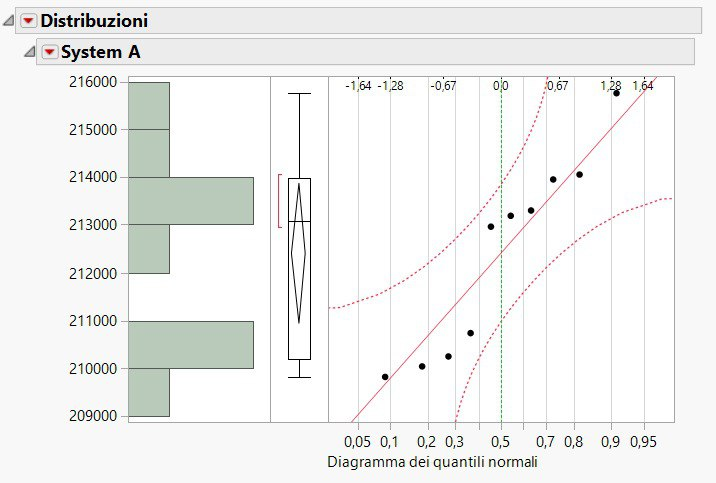
\includegraphics[width=\linewidth]{img/ch1/qqplot_a.png}
  \label{fig:qqplot_a}
\end{subfigure}%
\begin{subfigure}{.5\textwidth}
  \centering
  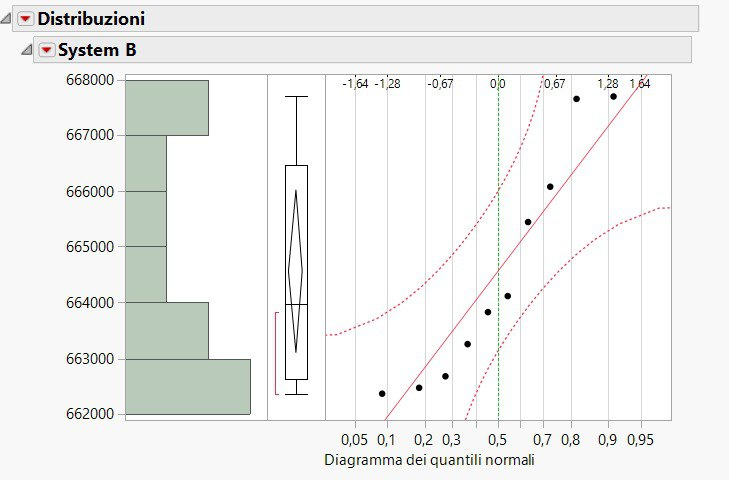
\includegraphics[width=\linewidth]{img/ch1/qqplot_b.png}
  \label{fig:qqplot_b}
\end{subfigure}
\caption{Plot quantile-quantile per Sistema A e Sistema B}
\label{fig:qqplot}
\end{figure}

Osservando i grafici in \cref{fig:qqplot}, si può concludere che entrambe le distribuzioni possono essere approssimate con una normale.

Sotto l'ipotesi di normalità, è possibile calcolare la \textit{sample size} usando la \cref{eq:sample_size}. 

\begin{equation}
    n = \left(\frac{z_{\alpha/2} \sigma}{E}\right)^2
    \label{eq:sample_size}
\end{equation}

In particolare, sfruttando i dati mostrati in \cref{table:10_samples}, scegliendo un intervallo di confidenza del $99\%$ e un errore pari a $0,01\%$ della media, è stato ottenuto il numero di campioni per entrambi i sistemi mostrati in \cref{tab:sample_size}.

\begin{table}[H]
\centering
    \begin{tabular}{|l|c|c|}
    \hline
    \multicolumn{1}{|c|}{\textbf{}} &
    \multicolumn{1}{c|}{\textbf{Sistema A}} & 
    \multicolumn{1}{c|}{\textbf{Sistema B}}  \tabularnewline \hline


Media & $644559.45$ & $212407.48$ \tabularnewline \hline
Dev.Std &$2047.23$ & $2051.20$
\tabularnewline \hline
\end{tabular}
\caption{Dati ottenuti prelevando in maniera preliminare $10$ campioni}
\label{table:10_samples}
\end{table}

\begin{table}[H]
\centering
    \begin{tabular}{|l|c|c|}
    \hline
    \multicolumn{1}{|c|}{\textbf{}} &
    \multicolumn{1}{c|}{\textbf{Sistema A}} & 
    \multicolumn{1}{c|}{\textbf{Sistema B}}  \tabularnewline \hline
    
Sample Size &$1.04$ & $10.27$ \tabularnewline \hline
\end{tabular}
\caption{Sample size ottenuta per entrambi i sistemi sotto l'ipotesi di normalità}
\label{tab:sample_size}
\end{table}

In base ai risultati ottenuti, si è deciso di procedere con $11$ campioni per entrambi i sistemi in modo da effettuare un \textit{paired test}.

\begin{table}[H]
\centering
    \begin{tabular}{|l|c|c|}
    \hline
    \multicolumn{1}{|c|}{\textbf{}} &
    \multicolumn{1}{c|}{\textbf{Sistema A}} & 
    \multicolumn{1}{c|}{\textbf{Sistema B}}  \tabularnewline \hline


Media & $644559.45$ & $212407.48$ \tabularnewline \hline
Dev.Std &$2047.23$ & $2051.20$ \tabularnewline \hline
\end{tabular}

\caption{Tabella riassuntiva dei due sistemi con $11$ campioni}
\end{table}

\section{Confronto tra i due sistemi}
Al fine di confrontare i due sistemi e verificare che le differenze tra le performance dei due sistemi sono statisticamente significative, si è scelto di operare un paired T-Test con $\alpha=0.05$ .

In \cref{fig:ris_ttest}, è mostrato il risultato del test, in cui appare chiaramente che tra i due sistemi c'è una differenza statistica.
\begin{figure}[H]
  \centering
  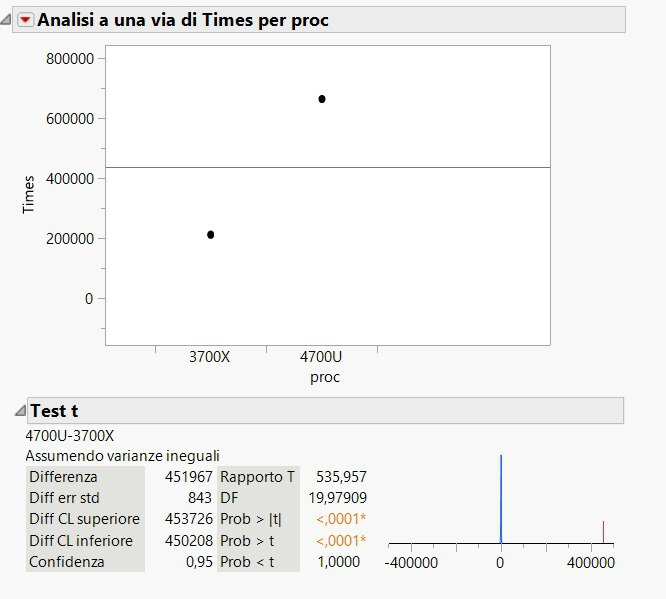
\includegraphics[width=\linewidth]{img/ch1/risultato_ttest.png}
  \caption{Risultati zero mean test con varianze ineguali}
  \label{fig:ris_ttest}
\end{figure}



\chapter{PCA e Clustering}

\section{Traccia}
Dato un workload reale, trovarne uno sintetico e:

\begin{itemize}
    \item Trovare il miglior trade-off (numero di componenti principali e numero di cluster) tra perdita di devianza e diminuzione della dimensione dei dati.
    \item Discutere le differenze tra l'applicazione della clusterizzazione con e senza PCA.
\end{itemize}

\subsection{Raccolta dati}
I dati sono stati raccolti su un sistema con le caratteristiche mostrate in \cref{tab:pca_specs}.

\begin{table}[H]
\centering
    \begin{tabular}{|c|p{0.7\linewidth} |}
    \hline
    \multicolumn{1}{|c|}{\textbf{Caratteristiche}} &
    \multicolumn{1}{c|}{\textbf{Sistema}}  \tabularnewline \hline


CPU & AMD Ryzen 7, 5700U 1.8 GHz, 8 Core 16T L3 8MB \tabularnewline \hline

RAM & DDR4 SODIMM 16GB, 3200 MHz \tabularnewline \hline

OS & Linux-liquorix v6.6.1, 6.6.1-zen1-1-zen \tabularnewline \hline
\end{tabular}
\caption{Tabella riassuntiva delle caratteristiche del sistema}
\label{tab:pca_specs}
\end{table}

I dati sono stati raccolti leggendo una volta al secondo per $10$ minuti il \textit{file} \textbf{\textit{/proc/meminfo}} usando il \textit{benchmark} \textbf{nBody} eseguito $16$ volte per sfruttare tutte i \textit{core} del sistema (inclusi quelli virtuali).

Alla fine della misurazione, è stato ottenuto un \textit{dataset} composto da $600$ righe che descriverà il \textit{workload} iniziale.

\subsection{Pre-processing}
Rimosse le colonne con valori non numerici, si è proceduto a normalizzare i dati usando lo \textit{z-score}, trasformando il \textit{dataset} iniziale in uno a media zero e varianza unitaria, applicando la \cref{eq:zscore} per ogni parametro $s$.

\begin{equation}
    x'_s = \frac{x_s - \mu_s} {\sigma_s}
    \label{eq:zscore}
\end{equation}

 in cui con $\sigma_s$ e $\mu_s$ si indicano rispettivamente la deviazione standard a la media del parametro $s$.

 \subsection{Principal component analysis}
L'analisi a componenti principali è una tecnica che serve ad operare una trasformazione di stato. In particolare, il risultato della PCA è un nuovo dataset formato da colonne incorrelate ordinate in termini di variazione spiegata. Formalmente, detta $y_j$ la \textit{j-esima} componente principale, questa si definisce secondo la \cref{eq:pca}.

\begin{equation}
    y_j =  \mathlarger{\sum}_{i=1}^n w_{ij} x_{i}
    \label{eq:pca}
\end{equation}

Le tecniche utilizzate per implementare questo procedimento mirano a calcolare il peso $w_{ij}$.

Tuttavia, le componenti principali non hanno nessun significato fisico e quindi non possono essere utilizzate in sostituzione del dataset inziale per fare delle valutazioni. A valle della
PCA è inoltre possibile eliminare le componenti con variazione spiegata minore in modo da diminuire la dimensionalità del dataset.

\subsection{Clustering}
Il clustering è una tecnica che raggruppa elementi del dataset utilizzando una certa misura di distanza. È stata applicato il metodo di \textbf{\textit{Ward}} che mira a minimizzare la varianza \textit{intra-cluster} e massimizzare quella \textit{inter-cluster}. 

In particolar, la devianza intra-cluster si definisce come:
\begin{equation*}
    \mathlarger{\sum}_{k=1}^K \mathlarger{\sum}_{i=1}^{n_k} ||X_i - \overline{X}_k||^2
\end{equation*}

Invece, la devianza \textit{inter-cluster} è definita come:
\begin{equation*}
     \mathlarger{\sum}_{k=1}^K n_k ||\overline{X}_k - \overline{X}||^2
\end{equation*}

 
Dove si è ipotizzata la presenza di $K$ cluster, ciascuno dei quali con $n_k$ elementi e, per ogni cluster, viene calcolato il centroide con:
\begin{equation*}
    \overline{X}_k = \frac{1}{n_k} \mathlarger{\sum}_{i=1}^{n_k} X_i
\end{equation*}
 
In particolare, è stata applicata la tecnica del \textbf{clustering gerarchico agglomerativo} che, ad ogni iterazione, prevede la fusione di due cluster a distanza minima. 
 

 \subsection{Analisi}
 Per valutare la qualità del \textit{clustering} in termini di devianza persa, si è deciso di comparare l'effetto della scelta delle componenti post-PCA, variando il numero di componenti principali prima di effettuare il \textit{clustering}. In particolare, sarà effettuata una comparazione per $n \in (4, 8, 12)$, con $n$ è indicato il numero di componenti principali, e $m \in (10, 20, 30, 40)$ con $m$ numero di cluster. I risultati sono riportati in \cref{tab:pca_cl_comp}.

\begin{table}[H]
\centering
    \begin{tabular}{|c|c|c|c|c|c|}
    \hline
    \multicolumn{1}{|c|}{\textbf{N. PC}} &
    \multicolumn{1}{|c|}{\textbf{Devianza \%}} &
    \multicolumn{4}{|c|}{\textbf{Cluster}} \tabularnewline \hline

 &  & \textbf{10} & \textbf{20} & \textbf{30}  & \textbf{40} \tabularnewline \hline
\multirow{3}{*}{\textbf{4}} & Post PCA & $72.38$ & $72.38$ & $72.38$ & $72.38$ \\[1.25ex]
& Post Cluster & $64.52$ & $67.83$ & $69.08$ & $69.58$ \\ [1.25ex]
& Totale persa & $35.48$ & $32.17$ & $30.92$ & $30.42$

\tabularnewline \hline

\multirow{3}{*}{\textbf{8}} & Post PCA & $90.44$ & $90.44$ & $90.44$ & $90.44$ \\ [1.25ex] 
& Post Cluster & $64.66$ & $75.01$ & $78.32$ & $80.33$ \\ [1.25ex]
& Totale persa & $35.34$ & $24.99$ & $21.68$ & $19.67$ 

\tabularnewline \hline

\multirow{3}{*}{\textbf{12}} & Post PCA & $97.13$ & $97.13$ & $97.13$ & $97.13$ \\ [1.25ex]
& Post Cluster & $70.11$ & $78.75$ & $82.04$ & $84.12$ \\ [1.25ex]
& Totale persa & $29.89$ & $21.25$ & $17.96$ & $15.88$

\tabularnewline \hline

\end{tabular}
\caption{Risultati ottenuti facendo variare il numero di componenti principali e il numero di cluster}

\label{tab:pca_cl_comp}
\end{table}

Come si osserva in \cref{fig:pca_cluster_lost_dev}, gli effetti del numero di componenti principali sono più marcati all'aumentare del numero di cluster. Infatti, con $m=10$ tra $4$ e $8$ componenti la differenza è quasi nulla, mentre con $n=12$ abbiamo uno scarto del $5 \%$. Invece, con $m=40$ lo scarto tra $4$ e $12$ componenti principali diventa del $15\%$. Inoltre, si può osservare che con $n=8$ e $n=12$ la differenza in devianza persa rimane circa costante al variare del numero di cluster.

Ovviamente scegliere un numero elevato di componenti principali permette di diminuire la devianza persa inizialmente e di selezionare un numero minore di cluster. D'altro canto un numero elevato di componenti principali può appesantire il processo di \textit{clustering}.

\begin{figure}[H]
    \centering
    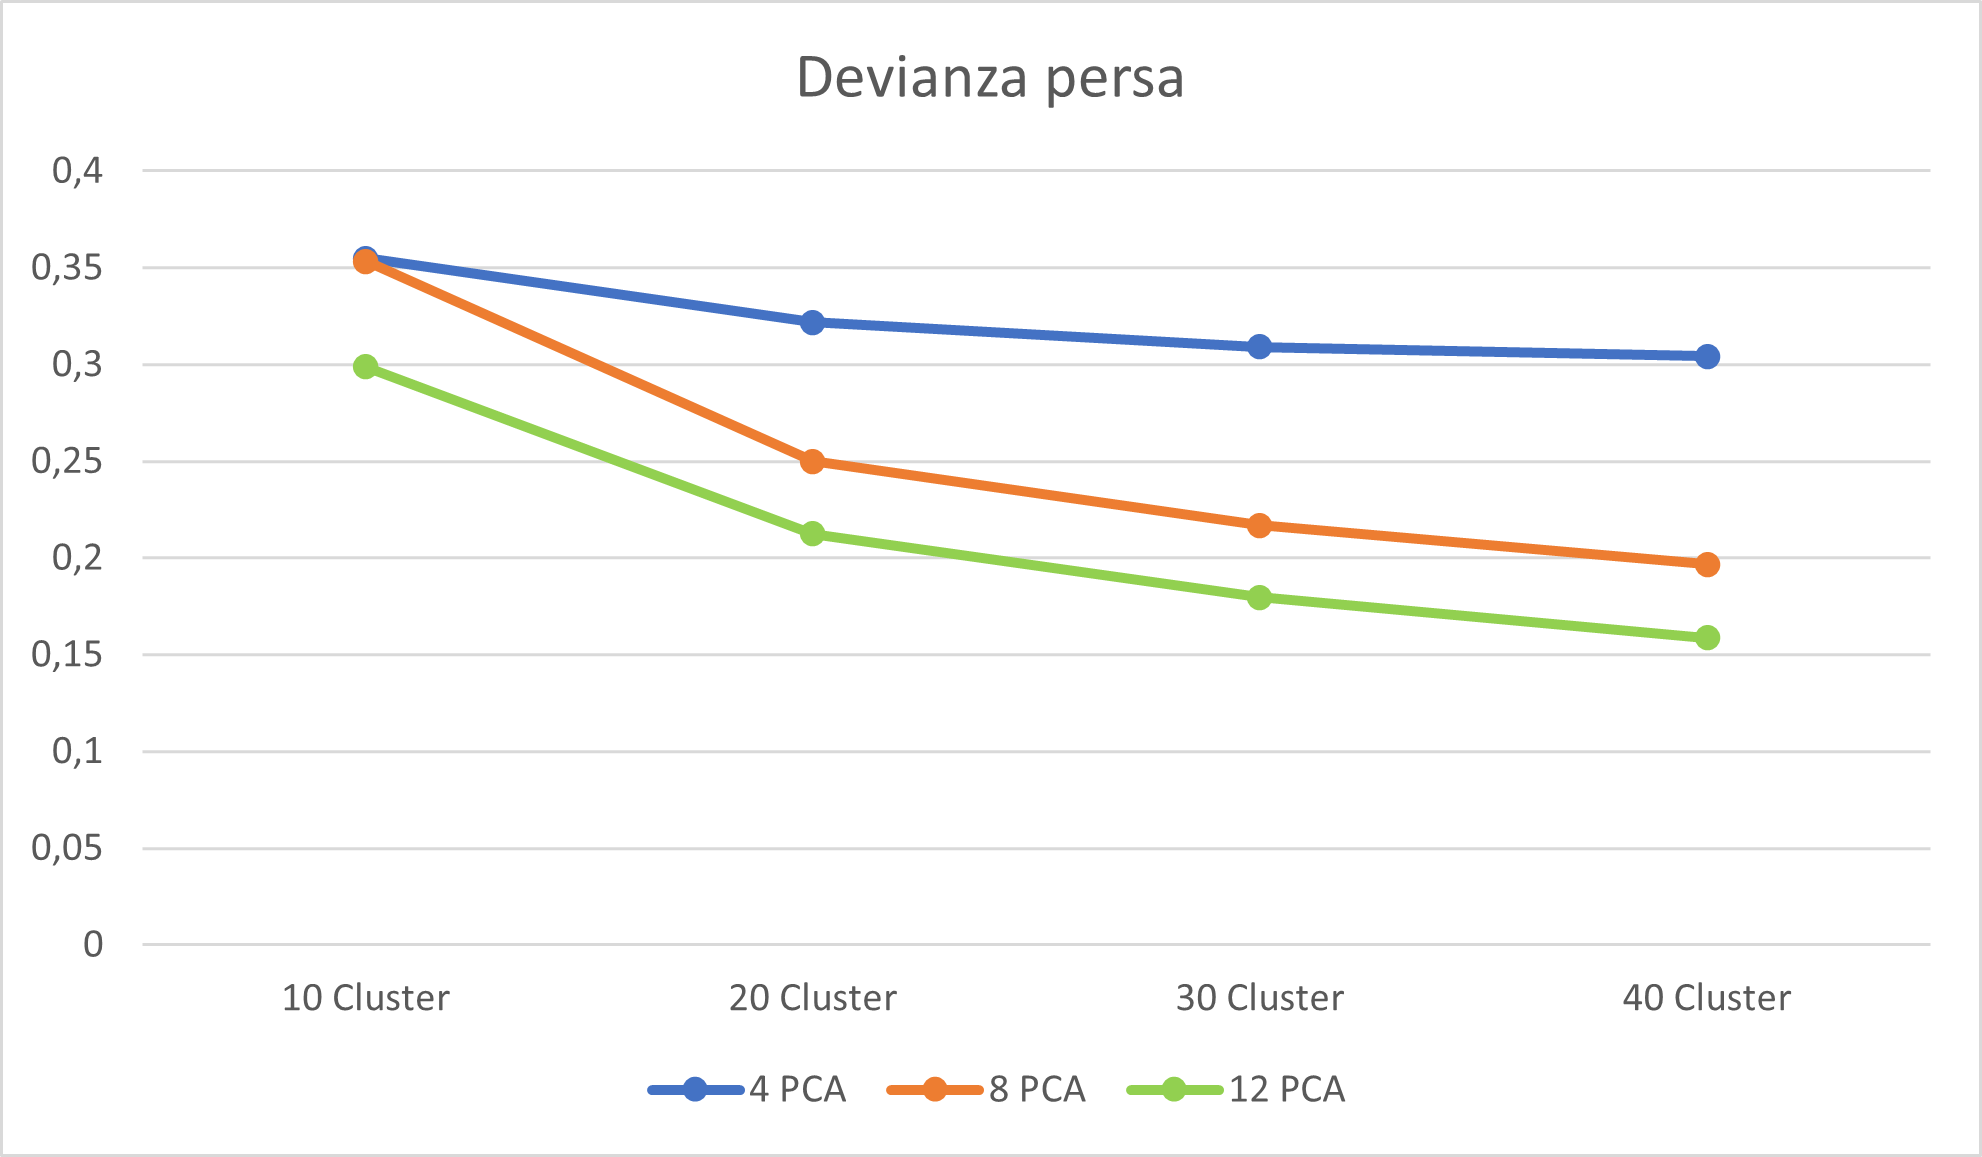
\includegraphics{img/ch2/lost_dev.png}
    \caption{Andamento devianza persa per numero di cluster e componenti principali}
    \label{fig:pca_cluster_lost_dev}
\end{figure}

\paragraph{Analisi outlier}Durante gli esperimenti si è notata la presenza di un
outlier corrispondente alla prima riga del dataset che nella magggior parte dei casi veniva assegnata ad un cluster isolato. Si è scelto di non scartare questa riga perchè ottenuta in condizioni di carico elevato.

\paragraph{Workload sintetico} Scegliendo $8$ componenti principali e $40$ cluster,
si è creato il workload sintetico (Figura \ref{fig:workload_synth}) con una devianza totale persa del $21.68\%$ con una
riduzione del dataset iniziale del $93.3\%$. L'elemento rappresentativo di ogni cluster è stato scelto randomicamente. 

\begin{figure}[H]
    \centering
    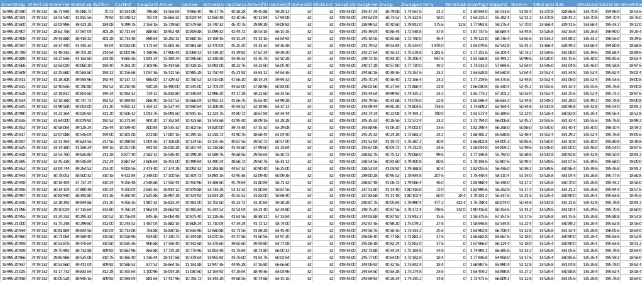
\includegraphics{img/ch2/synth_workload.png}
    \caption{Workload sintetico}
    \label{fig:workload_synth}
\end{figure}


\chapter{Web Server}

Analizzare le \textit{performance} di un \textit{web server}, effettuando le seguenti
attività:
\begin{itemize}
    \item \textbf{Capacity Test}: valutazione delle \textit{performance} del sistema al
    variare del carico di lavoro imposto;
    \item \textbf{Workload Characterization}: estrapolare un \textit{workload} sintetico
    a partire da un \textit{workload} reale e verificarne la significatività
    statistica dei rispettivi \textit{workload} di basso livello;
    \item \textbf{Design of Experiment}: verifica dell’influenza dei fattori sul
    \textit{response time} del sistema.
\end{itemize}

\section{Capacity Test}

Il web server è stato installato su una macchina virtuale \textit{VirtualBox} con le specifiche in \cref{tab:web_server_specs}. Le caratteristiche della macchina host sono mostrat in \cref{tab:host_specs}.

\begin{table}[H]
\centering
    \begin{tabular}{|c|p{0.3\linewidth}|}
    \hline
    \multicolumn{1}{|c|}{\textbf{Caratteristiche}} &
    \multicolumn{1}{c|}{\textbf{Server}}
    \tabularnewline \hline

CPU & 2 vCPU \tabularnewline \hline

RAM & 512 MB\tabularnewline \hline

OS & Alpine Linux 3.19, kernel 6.6.10-lts \tabularnewline \hline

Web server & Apache v2.4.58 \tabularnewline \hline
\end{tabular}
\caption{Tabella riassuntiva delle caratteristiche del Web Server}
\label{tab:web_server_specs}
\end{table}

\begin{table}[H]
\centering
    \begin{tabular}{|c|p{0.3\linewidth}|}
    \hline
    \multicolumn{1}{|c|}{\textbf{Caratteristiche}} &
    \multicolumn{1}{c|}{\textbf{Server}}
    \tabularnewline \hline

CPU & AMD Ryzen 5 2600, 6 core 12 threads \tabularnewline \hline

RAM & 16 GB, DDR4 3000 MHz\tabularnewline \hline

OS & Windows 10 \tabularnewline \hline
\end{tabular}
\caption{Tabella riassuntiva delle caratteristiche della macchina \textit{Host}}
\label{tab:host_specs}
\end{table}

Per il capacity test vengono prese in considerazione 2 metriche:
\begin{itemize}
    \item \textbf{Response Time}: intervallo di tempo che intercorre tra la richiesta
di una risorsa e la ricezione della risposta del sistema;
    \item \textbf{Throughput}: il numero di richieste per unità di tempo che
vengono servite dal server.
\end{itemize}

In particolare, sono state predisposte $10$ risorse di grandezza variabile da $64kB$ fino $1MB$.
Il capacity test ha come scopo quello di definire i punti di:
\begin{itemize}
    \item \textbf{Knee Capacity}: punto in cui la potenza (rapporto tra \textit{throughput}
    e \textit{response time}) è massima, dunque, rappresenta il miglior
    punto di funzionamento del sistema, poiché si ha il miglior tradeoff
    tra le due metriche adottate;
    \item \textbf{Usable Capacity}: punto in cui si ha il throughput massimo,
    senza superare i vincoli sul tempo di risposta. Dopo tale punto il
    throughput decresce al crescere del carico ed il tempo di risposta
    peggiora.
\end{itemize}
Attraverso uno script in \textit{Python} e il tool Jmeter, sono state raccolti campioni per livello di carico crescenti (regolando il valore \textit{Constant Throuhput Timer} (CTT)) effettuando 3 ripetezioni di ogni livello. 
Per assicurare l'indipendenza dei campioni è stato effettuato un riavvio del sistema tra una cattura e l'altra.
In particolare, è stata presa la media delle osservazioni come valore di riferimento per il campione ottenendo i dati in \cref{tab:capacity_results}. 
\begin{table}[H]

\centering
    \begin{tabular}{|c|c|c|}
    \hline
    \multicolumn{1}{|c|}{\textbf{CTT}} &
    \multicolumn{1}{|c|}{\textbf{Throughput (rps)}} &
    \multicolumn{1}{c|}{\textbf{Response time (millisecondi)}}  \tabularnewline \hline

200 & 3.56 & 72.96 \tabularnewline \hline
400 & 5.18 & 79.60 \tabularnewline \hline
600 & 4.93 & 113.71 \tabularnewline \hline
800 & 13.54 & 98.25 \tabularnewline \hline
1000 & 16.86 & 140.25 \tabularnewline \hline
1200 & 20.16 & 362.56 \tabularnewline \hline
1400 & 22.50 & 1901.10 \tabularnewline \hline
1600 & 18.35 & 3285.09 \tabularnewline \hline
\end{tabular}
\caption{Tabella riassuntiva delle caratteristiche dei due sistemi a cui è stato sottoposto il benchmark}
\label{tab:capacity_results}
\end{table}


\begin{figure}[H]
    \centering
    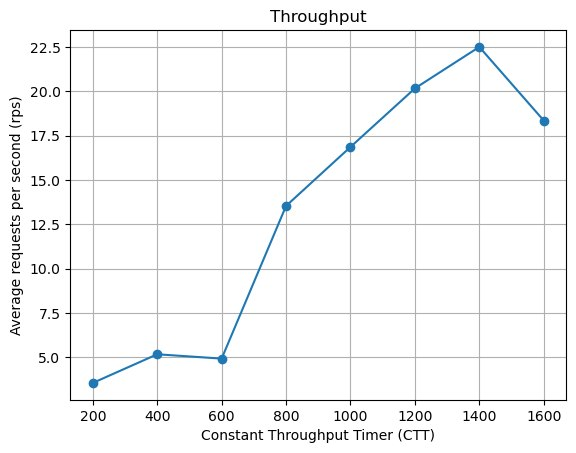
\includegraphics[width=0.8\textwidth]{img/ch3/throughput.jpeg}
    \caption{Throughput medio del web server al variare del carico}
    \label{fig:tput}
\end{figure}

\begin{figure}[H]
    \centering
    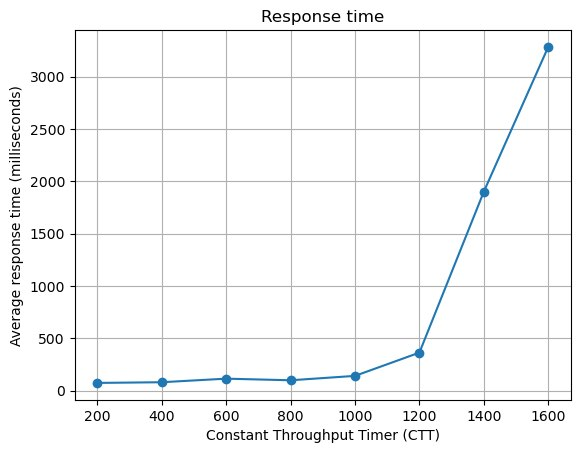
\includegraphics[width=0.8\textwidth]{img/ch3/responsetime.jpeg}
    \caption{Tempo di risposta medio del web server al variare del carico}
    \label{fig:responsetime}
\end{figure}

\begin{figure}[H]
    \centering
    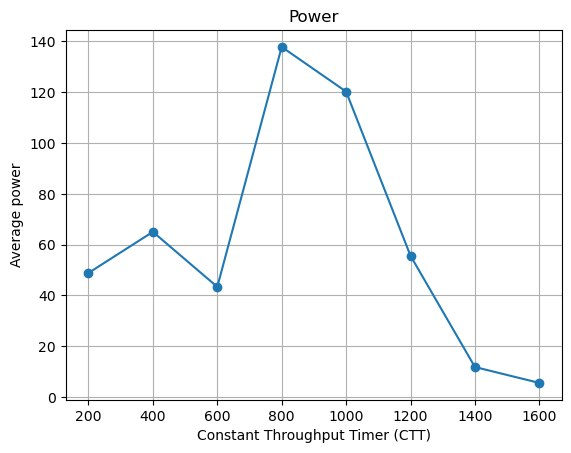
\includegraphics[width=0.8\textwidth]{img/ch3/power.jpeg}
    \caption{Andamento della potenza media del web server
    al variare del carico}
    \label{fig:power}
\end{figure}

A valle dei test svolti sono stati identificati i seguenti punti di interesse:
\begin{itemize}
    \item Knee Capacity: $800$ richieste al minuto;
    \item Usable capacity: $1400$ richieste al minuto;
\end{itemize}

\clearpage
\subsection{Bottleneck Performance}

Ai fini di identificare le risorse del sistema sottoposte a \textit{stress} maggiore sono state monitorate le risorse sul server con l'utility \textit{vmstat}. Analogamente ai parametri di alto livello, anche i parametri di sistema sono stati catturati effettuando $3$ osservazioni prendendo la media per ciascun punto. Tra le risorse monitorate sono presenti:
\begin{itemize}
    \item Utilizzo CPU;
    \item Numero di \textit{context switch};
    \item Consumo di memoria;
    \item Numero di interruzioni al secondo;
    \item \textit{Byte} inviati al secondo (kb/s);
\end{itemize}


In \cref{fig:low_level_parameters_cpu}, \cref{fig:low_level_parameters_mem}  e \cref{fig:low_level_io}, sono mostrati i grafici relativi agli andamenti medi dell'utilizzo del processore e della memoria e i parametri relativi alle prestazioni di I/O. 

\begin{figure}[H]
    \centering
    \begin{subfigure}{0.5\textwidth}
        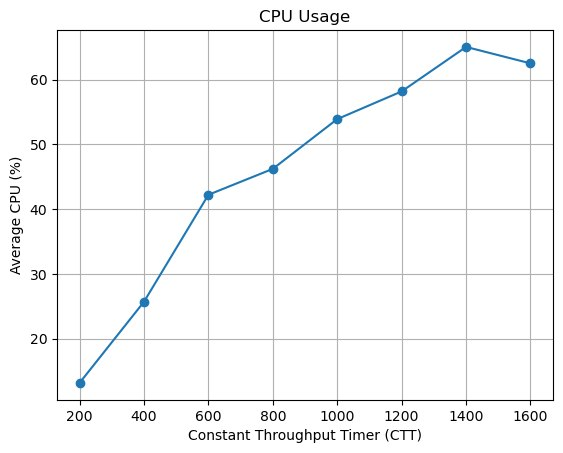
\includegraphics[width=0.95\linewidth]{img/ch3/cpu.jpeg}
        \caption{Andamento utilizzo medio CPU}
    \end{subfigure}\hfil
    \begin{subfigure}{0.5\textwidth}
        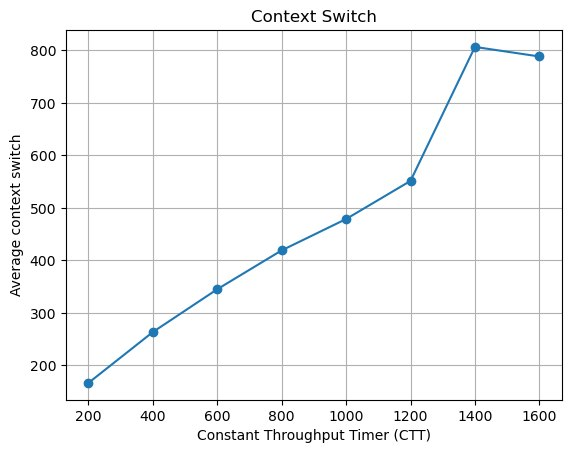
\includegraphics[width=0.95\linewidth]{img/ch3/contextswitch.jpeg}
        \caption{Numero medio di context switch}
    \end{subfigure}
    \caption{Andamento utilizzazione del processore e cambi di contesto}
    \label{fig:low_level_parameters_cpu}
\end{figure}

\begin{figure}[H]
    \centering
    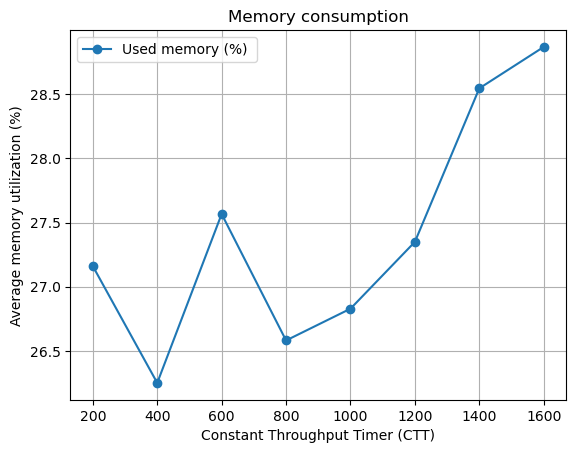
\includegraphics[width=0.6\linewidth]{img/ch3/mem.png}
    \caption{Andamento memoria utilizzata}
    \label{fig:low_level_parameters_mem}
\end{figure}

\begin{figure}[H]
    \centering
    \begin{subfigure}{0.5\textwidth}
        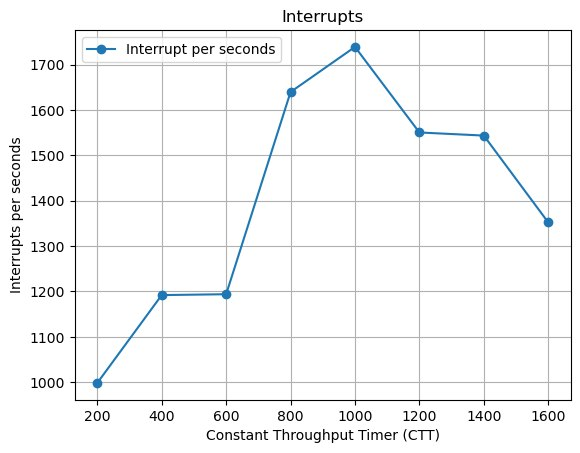
\includegraphics[width=0.95\linewidth]{img/ch3/interrupts.jpeg}
        \caption{Numero medio di interruzioni al secondo}
    \end{subfigure}\hfil
    \begin{subfigure}{0.5\textwidth}
        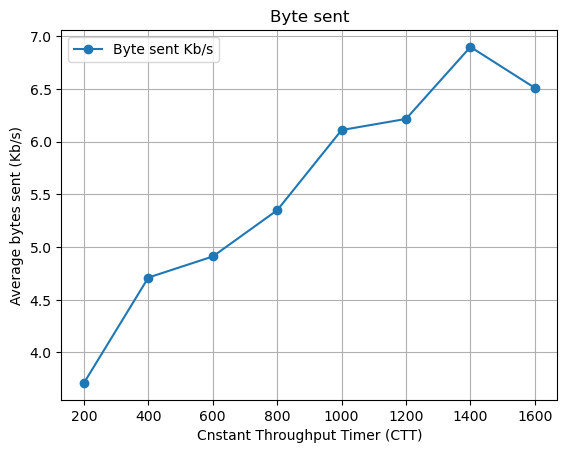
\includegraphics[width=0.95\linewidth]{img/ch3/byte_sent.png}
        \caption{Byte inviati al secondo (kb/s)}
    \end{subfigure}
    \caption{Andamento parametri riguardanti l'I/O}
    \label{fig:low_level_io}
\end{figure}


In particolare, si osserva che la saturazione del sistema che avviene dal  $CTT = 1400$, corrispondente al punto di \textit{usable capacity}, sembra essere causata dall'alto utilizzo della CPU. In figura \cref{fig:cpuvsmem} sono mostrate le percentuali di utilizzo di memoria e CPU messe a confronto, dove risulta chiaro che quest'ultima è il bottleneck.

\begin{figure}[H]
    \centering
    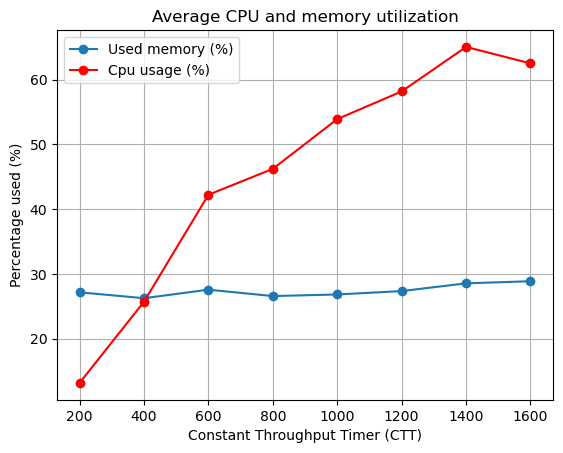
\includegraphics[width=0.8\linewidth]{img/ch3/cpu_vs_mem.png}
    \caption{Confronto percentuali di utilizzo di CPU e Memoria}
    \label{fig:cpuvsmem}
\end{figure}


\clearpage
\subsection{Fairness Index}

Si vuole valutare quanto il sistema sia equo nell'assegnazione delle risorse a più gruppi di utenti concorrenti. 
Per farlo, si calcola il \textit{Fairness Index} definito nella \cref{eq:fairness_index}.

\begin{equation}
    f = \frac{\left(\sum \limits _{i=1}^n x_i\right)^2}{n \cdot \sum \limits _{i=1}^n x_i^2}
    \label{eq:fairness_index}
\end{equation}

Sono stati creati i seguenti thread group su \textit{jmeter} per simulare l'attività degli utenti:

\begin{itemize}
    \item TG1: composto da $20$ utenti che fanno richieste leggere;
    \item TG2: composto da $15$ utenti che fanno richieste medie;
    \item TG3: composto da $5$ utenti che fanno richieste pesanti;  
\end{itemize}

Dopo aver somministrato il test al \textit{server}, è stata effettuata la misura del \textit{throughput} reale in base a ciascun \textit{thread group}. In particolare sono stati ottenuti i risultati in \cref{tab:fairness_results}.

\begin{table}[H]
\centering
    \begin{tabular}{|c|r|r|r|}
    \hline
    \multicolumn{1}{|c|}{\textbf{Thread group ID}} &
    \multicolumn{1}{|c|}{\textbf{TTP Ideale}} &
    \multicolumn{1}{|c|}{\textbf{TTP Misurato}}  &
    \multicolumn{1}{|c|}{\textbf{TTP Normalizzato}}
    \tabularnewline \hline

TG1 & $3.33$ & $3.38$ & $1.016$ \tabularnewline \hline
TG2 & $3.33$ & $3.38$ & $1.013$ \tabularnewline \hline
TG3 & $6.67$ & $6.54$ & $0.980$ \tabularnewline \hline

\end{tabular}
\caption{Tabella riassuntiva per il calcolo del \textit{fairness index} (con \textit{TTP} si è indicato il \textit{througphut}, espresso in richieste al secondo)}

\label{tab:fairness_results}
\end{table}

Il throughput normalizzato si calcola con la seguente formula:
\begin{equation*}
 T_{norm} = \frac{T_{misurato}}{T_{ideale}}
\end{equation*}

Applicando la \cref{eq:fairness_index}, è stato calcolato il \textit{fairness index} con un valore pari a $0.9997$.

\clearpage
\section{Workload characterization}

La \textit{Workload Characterization} ha lo scopo di generare un \textit{workload} sintetico partendo da uno reale. Sono state svolte le seguenti fasi, illustrate in \cref{fig:charcterization_flow}:
\begin{itemize}
    \item Creazione del \textit{workload} reale di di alto livello ($HL$ \textit{High Level}) e di basso livello ($LL$ \textit{Low Level});
    \item Creazione del \textit{workload} sintetico tramite la caratterizzazione di HL ($HL_c$) e di LL ($LL_c$);
    \item Applicazione del \textit{workload} $HL_c$ per raccogliere i parametri di basso livello $LL'$;
    \item caratterizzazione del \textit{workload} $LL \rightarrow LL_c$;
    \item Verifica della bontà della caratterizzazione del \textit{workload} di alto livello tramite test di ipotesi dei parametri di basso livello caratterizzati $LL'_c \rightarrow LL'_c$;
\end{itemize}

\begin{figure}[H]
    \centering
    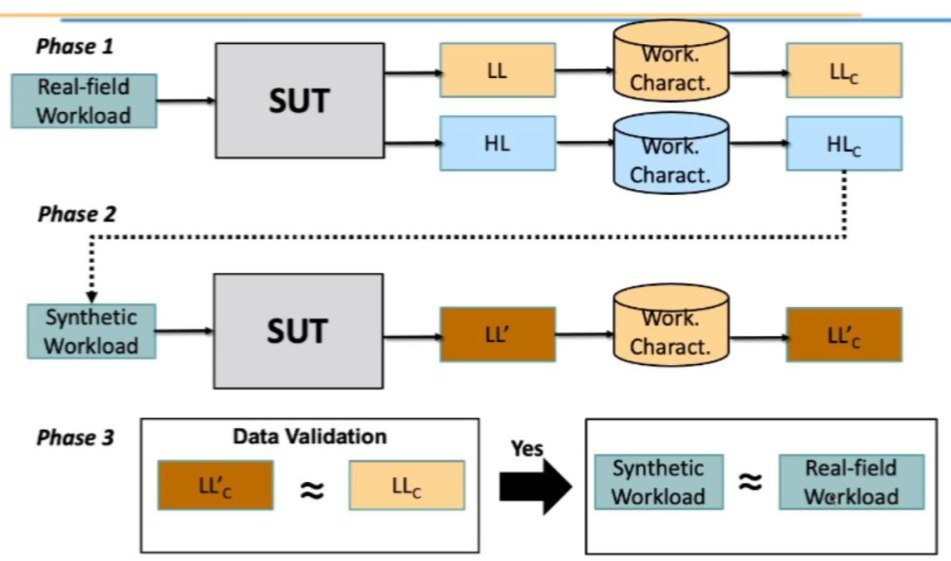
\includegraphics[width=0.8\textwidth]{img/ch3/characterization.jpg}
    \caption{Workload Characterization}
    \label{fig:charcterization_flow}
\end{figure}

\subsection{Workload reale}
Attraverso \textit{Jmeter} è stata generata una traccia di traffico reale con il \textit{web server} configurato per avere $20$ risorse di dimensione variabile da $64 kB$ a $3 MB$. Inoltre, è stata ipotizzata la presenza di $5$ gruppi di utenti distinti aventi accesso solo a $10$ risorse. I gruppi sono stati configurati secondo la \cref{tab:wc_real}. Ciascun gruppo di utenti effettua richieste per $5$ minuti.


\begin{table}[H]
\centering
    \begin{tabular}{|c|c|c|}
    \hline
    \multicolumn{1}{|c|}{\textbf{Thread group ID}} &
    \multicolumn{1}{|c|}{\textbf{Numero utenti}} &
    \multicolumn{1}{|c|}{\textbf{Richieste al minuto (CTT)}}
    \tabularnewline \hline

TG1 & $20$ & $400$ \tabularnewline \hline
TG2 & $15$ & $500$ \tabularnewline \hline
TG3 & $10$ & $600$ \tabularnewline \hline
TG4 & $25$ & $200$ \tabularnewline \hline
TG5 & $40$ & $150$ \tabularnewline \hline
\end{tabular}
\caption{Tabella riassuntiva per la generazione della traccia di traffico reale}

\label{tab:wc_real}
\end{table}

Inoltre, durante la generazione della traccia di traffico reale sono stati collezionati parametri di basso livello sul server attraverso l'\textit{utility} \textit{vmstat}.

In \cref{tab:tg1_real}, sono riportate le richieste effettuate dal \textit{TG1}.

\begin{table}[H]
\centering
    \begin{tabular}{|c|c|c|}
    \hline
    \multicolumn{1}{|c|}{\textbf{Risorsa}} &
    \multicolumn{1}{|c|}{\textbf{Nome}} &
    \multicolumn{1}{|c|}{\textbf{Dimensione}}
    \tabularnewline \hline

1 & 1.png & 64 KB \tabularnewline \hline
2 & 5.pdf & 452 KB \tabularnewline \hline
3 & 10.pdf & 771 KB \tabularnewline \hline
4 & 15.pdf & 1.3 MB \tabularnewline \hline
5 & 17.pdf & 1.7 MB \tabularnewline \hline
6 & 2.html & 127 KB \tabularnewline \hline
7 & 11.pdf & 857 KB \tabularnewline \hline
8 & 19.pdf & 2.6 MB \tabularnewline \hline
9 & 4.png & 374 KB \tabularnewline \hline
10 & 8.pdf & 588 KB \tabularnewline \hline
\end{tabular}
\caption{Richieste effettuate da TG1}
\label{tab:tg1_real}
\end{table}

In \cref{tab:tg2_real}, sono riportate le richieste effettuate dal \textit{TG2}.

\begin{table}[H]
\centering
    \begin{tabular}{|c|c|c|}
    \hline
    \multicolumn{1}{|c|}{\textbf{Risorsa}} &
    \multicolumn{1}{|c|}{\textbf{Nome}} &
    \multicolumn{1}{|c|}{\textbf{Dimensione}}
    \tabularnewline \hline

1 & 3.docx & 230 KB   \tabularnewline \hline
2 & 7.pdf & 581 KB  \tabularnewline \hline
3 & 10.pdf & 771 KB \tabularnewline \hline
4 & 14.pdf & 1.2 MB \tabularnewline \hline
5 & 18.pdf & 2.1 MB \tabularnewline \hline
6 & 20.pdf & 2.9 MB \tabularnewline \hline
7 & 6.pdf & 528 KB  \tabularnewline \hline
8 & 11.pdf & 857 KB \tabularnewline \hline
9 & 16.pdf & 1.7 MB \tabularnewline \hline
10 & 2.html & 127 KB \tabularnewline \hline
\end{tabular}
\caption{Richieste effettuate da TG2}
\label{tab:tg2_real}
\end{table}

In \cref{tab:tg3_real}, sono riportate le richieste effettuate dal \textit{TG3}.

\begin{table}[H]
\centering
    \begin{tabular}{|c|c|c|}
    \hline
    \multicolumn{1}{|c|}{\textbf{Risorsa}} &
    \multicolumn{1}{|c|}{\textbf{Nome}} &
    \multicolumn{1}{|c|}{\textbf{Dimensione}}
    \tabularnewline \hline

1 & 7.pdf & 64 KB \tabularnewline \hline
2 & 17.pdf & 1.7 MB \tabularnewline \hline
3 & 13.pdf & 995 KB \tabularnewline \hline
4 & 9.pdf & 659 KB \tabularnewline \hline
5 & 4.png & 374 KB \tabularnewline \hline
6 & 18.pdf & 2.1 MB \tabularnewline \hline
7 & 12.pdf & 881 KB \tabularnewline \hline
8 & 6.pdf & 528 KB \tabularnewline \hline
9 & 14.pdf & 1.2 MB \tabularnewline \hline
10 & 19.pdf & 771 KB \tabularnewline \hline
\end{tabular}
\caption{Richieste effettuate da TG3}
\label{tab:tg3_real}
\end{table}

In \cref{tab:tg4_real}, sono riportate le richieste effettuate dal \textit{TG4}.
\begin{table}[H]
\centering
    \begin{tabular}{|c|c|c|}
    \hline
    \multicolumn{1}{|c|}{\textbf{Risorsa}} &
    \multicolumn{1}{|c|}{\textbf{Nome}} &
    \multicolumn{1}{|c|}{\textbf{Dimensione}}
    \tabularnewline \hline

1 & 4.png & 374 KB  \tabularnewline \hline
2 & 14.pdf & 1.2 MB \tabularnewline \hline
3 & 2.html & 127 KB  \tabularnewline \hline
4 & 12.pdf & 881 KB \tabularnewline \hline
5 & 9.pdf & 659 KB  \tabularnewline \hline
6 & 6.pdf & 528 KB  \tabularnewline \hline
7 & 2.html & 127 KB  \tabularnewline \hline
8 & 15.pdf & 1.3 MB \tabularnewline \hline
9 & 18.pdf & 2.1 MB \tabularnewline \hline
10 & 7.pdf & 581 KB \tabularnewline \hline
\end{tabular}
\caption{Richieste effettuate da TG4}
\label{tab:tg4_real}
\end{table}

In \cref{tab:tg5_real}, sono riportate le richieste effettuate dal \textit{TG5}.
\begin{table}[H]
\centering
    \begin{tabular}{|c|c|c|}
    \hline
    \multicolumn{1}{|c|}{\textbf{Risorsa}} &
    \multicolumn{1}{|c|}{\textbf{Nome}} &
    \multicolumn{1}{|c|}{\textbf{Dimensione}}
    \tabularnewline \hline

1 & 3.docx & 230 KB \tabularnewline \hline
2 & 7.pdf & 581 KB \tabularnewline \hline
3 & 9.pdf & 659 KB \tabularnewline \hline
4 & 4.png & 374 KB \tabularnewline \hline
5 & 15.pdf & 1.3 MB \tabularnewline \hline
6 & 11.pdf & 857 KB \tabularnewline \hline
7 & 4.png & 374 KB \tabularnewline \hline
8 & 12.pdf & 588 KB \tabularnewline \hline
9 & 4.png & 374 KB \tabularnewline \hline
10 & 19.pdf & 771 KB \tabularnewline \hline

\end{tabular}
\caption{Richieste effettuate da TG5}
\label{tab:tg5_real}
\end{table}

\subsection{Caratterizzazione del \textit{workload} reale}

\paragraph{Parametri di alto livello ($HL \rightarrow HL_c$)}
Terminata la fase di cattura, è stato caratterizzato il \textit{file csv} prodotto da \textit{jmeter} attraverso le operazioni di \textit{PCA} e \textit{Clustering}. In particolare, escluse le colonne non numeriche, sono state scelte $4$ componenti principali mantenendo circa il $95\%$ di devianza del \textit{dataset} iniziale. Successivamente, sono stati scelti $30$ cluster per raggruppare le richieste del \textit{workload} reale. In particolare, per ogni cluster è stata scelta la richiesta più rappresentativa (quella che compare un numero maggiore di volte) e in caso di sovrapposizione si è proceduto a scegliere le successive. In questo modo, mantenendo l'$89\%$ della devianza iniziale, si è passati da $50$ tipi di richieste a $30$ semplificando il \textit{workload iniziale} del $40\%$.


In \cref{tab:tg1_synthetic}, sono riportate le richieste effettuate dal \textit{TG1}.

\begin{table}[H]
\centering
    \begin{tabular}{|c|c|c|}
    \hline
    \multicolumn{1}{|c|}{\textbf{Risorsa}} &
    \multicolumn{1}{|c|}{\textbf{Nome}} &
    \multicolumn{1}{|c|}{\textbf{Dimensione}}
    \tabularnewline \hline

2 & 5.pdf & 452 KB \tabularnewline \hline
3 & 10.pdf & 771 KB \tabularnewline \hline
4 & 15.pdf & 1.3 MB \tabularnewline \hline
5 & 17.pdf & 1.7 MB \tabularnewline \hline
7 & 11.pdf & 857 KB \tabularnewline \hline
8 & 19.pdf & 2.6 MB \tabularnewline \hline
9 & 4.png & 374 KB \tabularnewline \hline
\end{tabular}
\caption{Richieste effettuate da TG1 per il workload sintetico}
\label{tab:tg1_synthetic}
\end{table}

In \cref{tab:tg2_synthetic}, sono riportate le richieste effettuate dal \textit{TG2}.

\begin{table}[H]
\centering
    \begin{tabular}{|c|c|c|}
    \hline
    \multicolumn{1}{|c|}{\textbf{Risorsa}} &
    \multicolumn{1}{|c|}{\textbf{Nome}} &
    \multicolumn{1}{|c|}{\textbf{Dimensione}}
    \tabularnewline \hline

1 & 3.docx & 230 KB   \tabularnewline \hline
2 & 7.pdf & 581 KB  \tabularnewline \hline
3 & 10.pdf & 771 KB \tabularnewline \hline
4 & 14.pdf & 1.2 MB \tabularnewline \hline
5 & 18.pdf & 2.1 MB \tabularnewline \hline
6 & 20.pdf & 2.9 MB \tabularnewline \hline
7 & 6.pdf & 528 KB  \tabularnewline \hline
8 & 11.pdf & 857 KB \tabularnewline \hline
9 & 16.pdf & 1.7 MB \tabularnewline \hline
10 & 2.html & 127 KB \tabularnewline \hline
\end{tabular}
\caption{Richieste effettuate da TG2 per il workload sintetico}
\label{tab:tg2_synthetic}
\end{table}

In \cref{tab:tg3_synthetic}, sono riportate le richieste effettuate dal \textit{TG3}.

\begin{table}[H]
\centering
    \begin{tabular}{|c|c|c|}
    \hline
    \multicolumn{1}{|c|}{\textbf{Risorsa}} &
    \multicolumn{1}{|c|}{\textbf{Nome}} &
    \multicolumn{1}{|c|}{\textbf{Dimensione}}
    \tabularnewline \hline

1 & 7.pdf & 64 KB \tabularnewline \hline
2 & 17.pdf & 1.7 MB \tabularnewline \hline
3 & 13.pdf & 995 KB \tabularnewline \hline
4 & 9.pdf & 659 KB \tabularnewline \hline
6 & 18.pdf & 2.1 MB \tabularnewline \hline
7 & 12.pdf & 881 KB \tabularnewline \hline
8 & 6.pdf & 528 KB \tabularnewline \hline
9 & 14.pdf & 1.2 MB \tabularnewline \hline
10 & 19.pdf & 771 KB \tabularnewline \hline
\end{tabular}
\caption{Richieste effettuate da TG3 per il workload sintetico}
\label{tab:tg3_synthetic}
\end{table}

In \cref{tab:tg4_synthetic}, sono riportate le richieste effettuate dal \textit{TG4}.
\begin{table}[H]
\centering
    \begin{tabular}{|c|c|c|}
    \hline
    \multicolumn{1}{|c|}{\textbf{Risorsa}} &
    \multicolumn{1}{|c|}{\textbf{Nome}} &
    \multicolumn{1}{|c|}{\textbf{Dimensione}}
    \tabularnewline \hline

3 & 2.html & 127 KB  \tabularnewline \hline
\end{tabular}
\caption{Richieste effettuate da TG4 per il workload sintetico}
\label{tab:tg4_synthetic}
\end{table}

In \cref{tab:tg5_synthetic}, sono riportate le richieste effettuate dal \textit{TG5}.
\begin{table}[H]
\centering
    \begin{tabular}{|c|c|c|}
    \hline
    \multicolumn{1}{|c|}{\textbf{Risorsa}} &
    \multicolumn{1}{|c|}{\textbf{Nome}} &
    \multicolumn{1}{|c|}{\textbf{Dimensione}}
    \tabularnewline \hline

1 & 3.docx & 230 KB \tabularnewline \hline
5 & 15.pdf & 1.3 MB \tabularnewline \hline
10 & 19.pdf & 771 KB \tabularnewline \hline

\end{tabular}
\caption{Richieste effettuate da TG5 per il workload sintetico}
\label{tab:tg5_synthetic}
\end{table}

\paragraph{Parametri di basso livello ($LL \rightarrow LL_c$)}
Similmente a quanto fatto per i parametri di alto livello, sono stati effettuati $PCA$ e $Clustering$ per i dati raccolti con \textit{vmstat}. In particolare, sono state scelte $6$ componenti principali e $20$ cluster perdendo circa il $13\%$ di devianza totale. Inoltre, in preparazione al test di ipotesi sono state verificate la normalità e l'omoschedasticità per le componenti principali calcolate.

\begin{figure}[H]
    \centering
    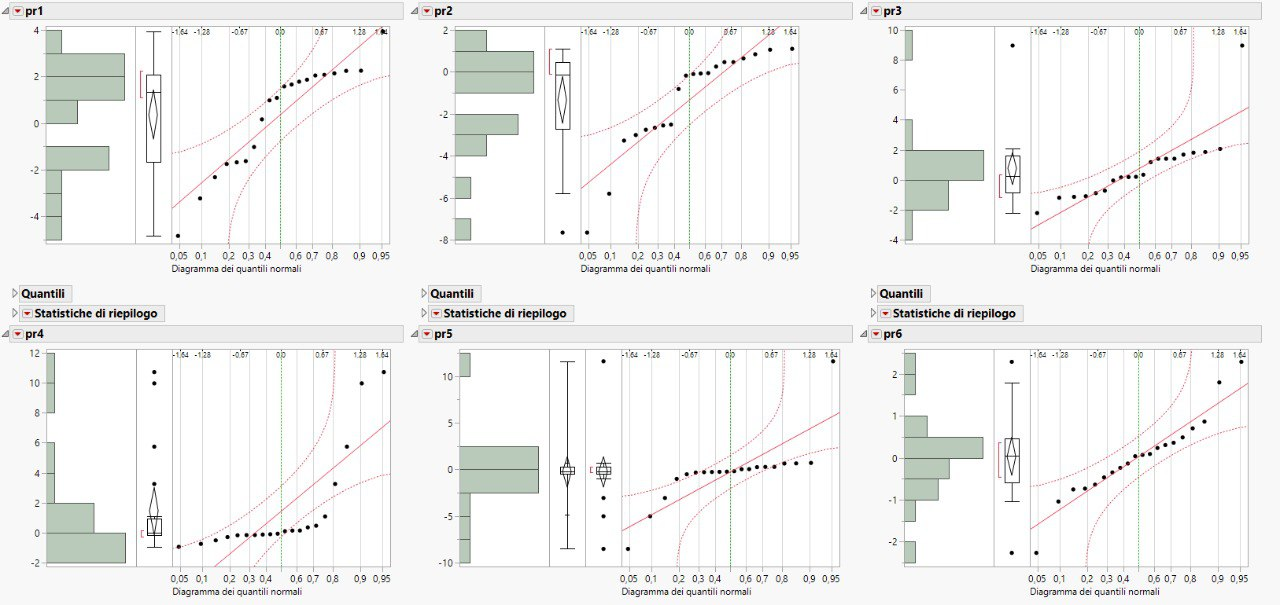
\includegraphics[width=\textwidth]{img/ch3/real.jpg}
    \caption{Test di normalità visivo delle componenti principali. Le componenti $1,2,3,6$ risultano normali.}
    \label{fig:real_qqplot}
\end{figure}

In \cref{fig:real_qqplot}, si osserva come le componente principali $1,2,3,6$ sembrano seguire la distribuzione normale, dato che i quantili sono all'interno delle bande. Tuttavia, data la presenza di alcuni punti in prossimità delle bande, si è scelto di procedere con il test di Shapiro-Wilk i cui risultati sono riportati in
\cref{tab:ll_norm}.

\begin{table}[H]
\centering
    \begin{tabular}{|c|c|r|}
    \hline
    \multicolumn{1}{|c|}{\textbf{Componente principale}} &
    \multicolumn{1}{|c|}{\textbf{Esito Shapiro-Wilk}} &
    \multicolumn{1}{|c|}{\textbf{P-value}}
    \tabularnewline \hline

1 & 0 & 0.053 \tabularnewline \hline
2 & 1 & 0.005 \tabularnewline \hline
3 & 1 & 0.0002 \tabularnewline \hline
6 & 0 & 0.485 \tabularnewline \hline
\end{tabular}
\caption{Risultati test normalità per le componenti $1,2,3,6$}
\label{tab:ll_norm}
\end{table}

È stata dimostrata l'omoschedasticità mediante il \textit{Two-sample F-test} in \cref{tab:ll_omoschedasticit} per le componenti $1,6$ risultate normali dal test precedente.

\begin{table}[H]
\centering
    \begin{tabular}{|c|c|r|}
    \hline
    \multicolumn{1}{|c|}{\textbf{Componente principale}} &
    \multicolumn{1}{|c|}{\textbf{Esito (H)}} &
    \multicolumn{1}{|c|}{\textbf{P-value}}
    \tabularnewline \hline

1 & 0 & 0.7227 \tabularnewline \hline
6 & 0 & 0.5020 \tabularnewline \hline
\end{tabular}
\caption{Risultati omoschedasticità componenti $1,6$}
\label{tab:ll_omoschedasticit}
\end{table}

\subsection{Validazione del workload sintetico ($LL' \rightarrow LL'_c$)}
Generato il \textit{workload} sintetico, questo è stato applicato al server collezionando nuovamente i parametri di basso livello ($LL'$) con \textit{vmstat}. Quindi si sono calcolate le $6$ componenti principali e si è effettuato il raggruppamento delle richieste in $20$ cluster, in maniera analoga a $LL_c$, ottenendo $LL'_c$.

\begin{figure}[H]
    \centering
    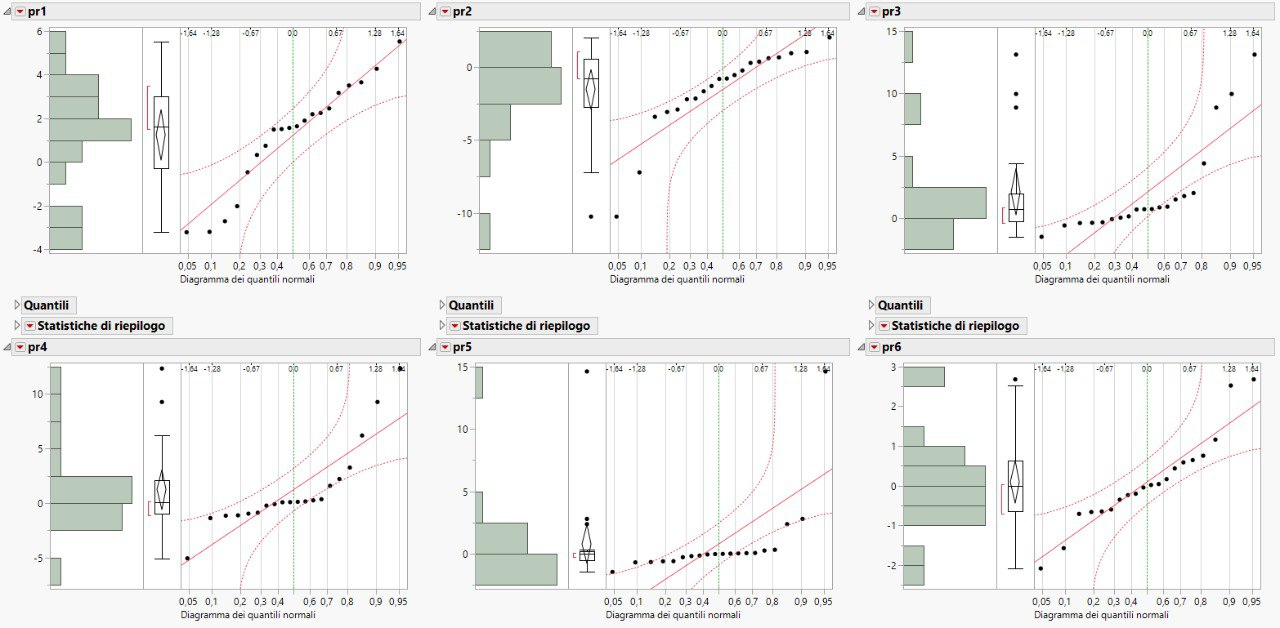
\includegraphics[width=\textwidth]{img/ch3/synth.jpg}
    \caption{Test di normalità visivo delle componenti principali.}
    \label{fig:synt_qqplot}
\end{figure}

Per le componenti $1,6$ è stata verificata la normalità sia visivamente che con il test di Shapiro-Wilk i cui
risultati sono messi in \cref{tab:ll1_norm}.
\begin{table}[H]
\centering
    \begin{tabular}{|c|c|r|}
    \hline
    \multicolumn{1}{|c|}{\textbf{Componente principale}} &
    \multicolumn{1}{|c|}{\textbf{Esito Shapiro-Wilk}} &
    \multicolumn{1}{|c|}{\textbf{P-value}}
    \tabularnewline \hline

1 & 0 & 0.218 \tabularnewline \hline
6 & 0 & 0.212 \tabularnewline \hline
\end{tabular}
\caption{Risultati test normalità per le componenti $1,6$}
\label{tab:ll1_norm}
\end{table}

È stata poi verificata l'omoschedasticità attraverso il \textit{Two-sample F-test} (\cref{tab:ll1_omoschedasticit}).

\begin{table}[H]
\centering
    \begin{tabular}{|c|c|r|}
    \hline
    \multicolumn{1}{|c|}{\textbf{Componente principale}} &
    \multicolumn{1}{|c|}{\textbf{Esito (H)}} &
    \multicolumn{1}{|c|}{\textbf{P-value}}
    \tabularnewline \hline

1 & 0 & 0.6487 \tabularnewline \hline
6 & 0 & 0.7826 \tabularnewline \hline
\end{tabular}
\caption{Risultati omoschedasticità componenti $1,6$}
\label{tab:ll1_omoschedasticit}
\end{table}


\paragraph{Test di ipotesi} Infine, si è proceduto nell'applicazione del test di ipotesi per ciascuna componente principale. Visti i risultati in \cref{tab:validation_test}, è possibile quindi concludere che non ci sono differenze statistiche tra il \textit{workload} sintetico e quello reale da cui si è partiti.

\begin{table}[H]
\centering
    \begin{tabular}{|c|c|c|r|}
    \hline
    \multicolumn{1}{|c|}{\textbf{Componenti principali}} &
    \multicolumn{1}{|c|}{\textbf{Tipologia di test}} &
    \multicolumn{1}{|c|}{\textbf{Esito(H)}} &
    \multicolumn{1}{|c|}{\textbf{P-value}}
    \tabularnewline \hline

PR1 & T-Test Equal Variance  & 0 & 0.0595 \tabularnewline \hline
PR2 & Wilcoxon rank sum  & 0 & 0.9246 \tabularnewline \hline
PR3 & Wilcoxon rank sum  & 0 & 0.4735 \tabularnewline \hline
PR4 & Wilcoxon rank sum  & 0 & 0.7353 \tabularnewline \hline
PR5 & Wilcoxon rank sum  & 0 & 0.6168 \tabularnewline \hline
PR6 & T-Test Equal Variance  & 0 & 0.8559 \tabularnewline \hline
\end{tabular}
\caption{Risultati per la validazione del workload sintetico}
\label{tab:validation_test}
\end{table}



\newpage
\section{Design of experiment}

Il DOE, acronimo di "Design of Experiments", indica una metodologia statistica e scientifica utilizzata per pianificare, condurre e analizzare esperimenti scientifici o industriali. L'obiettivo principale di un DOE è ottimizzare il processo, migliorare la qualità del prodotto o identificare i fattori chiave che influenzano una risposta specifica, minimizzando il numero di esperimenti necessari.

In questo esperimento si vuole studiare l'impatto dei fattori \textit{Request Rate} e \textit{Page type} sulla variabile di risposta \textit{Response time}. Per identificare i livelli del \textit{request rate}, si è partiti dalla \textit{usable capacity} calcolata durante \textit{capacity test}.

È stato impiegato un design sperimentale a $2$ fattori, ciascuno dei quali può assumere $3$ livelli categorici, effettuando e $5$ ripetizioni.

\begin{itemize}
    \item Request rate:
    \begin{itemize}
        \item 350 richieste al minuto, corrispondenti al 25\% della usable capacity.
        \item 700 richieste al minuto, corrispondenti al 50\% della usable capacity.
        \item 1050 richieste al minuto, corrispondenti al 75\% della usable capacity.
    \end{itemize}

    \item Page type:
    \begin{itemize}
        \item Small: 127KB
        \item Medium: 452KB
        \item Large: 1.2MB 
    \end{itemize}
\end{itemize}

Quindi con i parametri scelti, si sono realizzati $45$ esperimenti i cui risultati, al variare del \textit{Request rate} sono riportati nelle seguenti tabelle .

\begin{figure}[H]
    \centering
    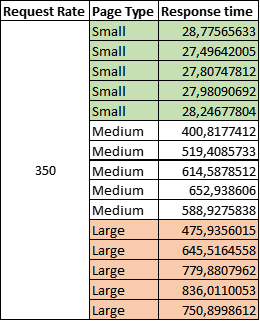
\includegraphics[width=0.4\textwidth]{img/ch3/doe350.png}
    \caption{Risultati per CTT 350}
\end{figure}

\begin{figure}[H]
    \centering
    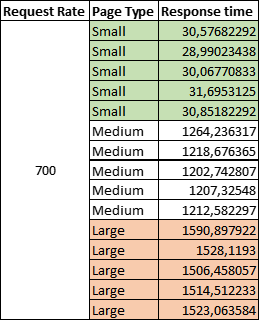
\includegraphics[width=0.4\textwidth]{img/ch3/doe700.png}
    \caption{Risultati per CTT 700}
\end{figure}

\begin{figure}[H]
    \centering
    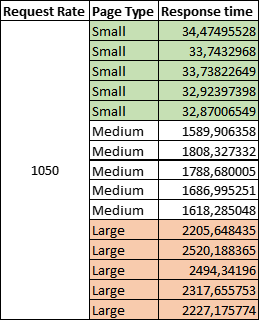
\includegraphics[width=0.4\textwidth]{img/ch3/doe1050.png}
    \caption{Risultati per CTT 1050}
\end{figure}


Successivamente, è stata effettuata una stima regressiva, il cui grafico è visibile in figura \cref{fig:modello_completo} con interazione dei fattori.

\begin{figure}[H]
    \centering
    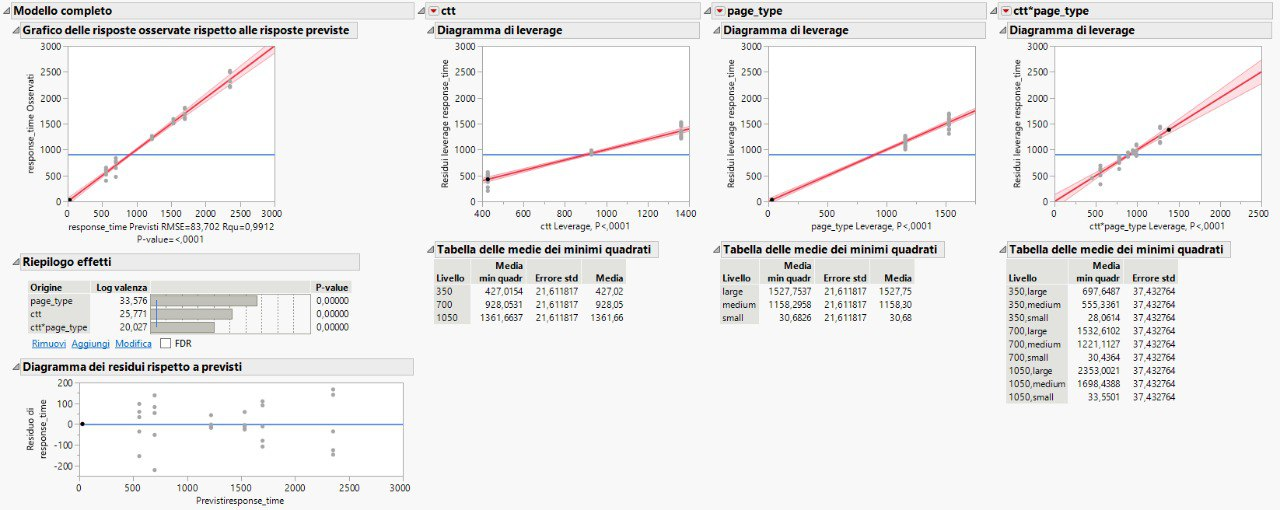
\includegraphics[width=\textwidth]{img/ch3/modello_completo.png}
    \caption{Stima del modello completo}
    \label{fig:modello_completo}
\end{figure}

In \cref{fig:analisi_varianza} e \cref{fig:test_degli_effetti}, sono riportati i dettagli del modello stimato, con la somma dei quadrati di tutti i parametri.

\begin{figure}[H]
    \centering
    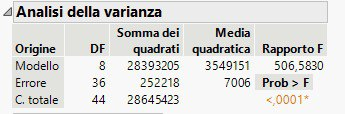
\includegraphics[width=0.6\textwidth]{img/ch3/analisi_varianza.png}
    \caption{Analisi Varianza}
    \label{fig:analisi_varianza}
\end{figure}

\begin{figure}[H]
    \centering
    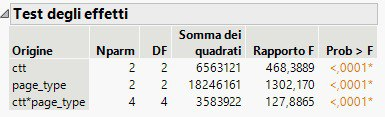
\includegraphics[width=0.6\textwidth]{img/ch3/test_degli_effetti.png}
    \caption{Test degli Effetti}
    \label{fig:test_degli_effetti}
\end{figure}

\paragraph{Importanza}
Un fattore è importante se esprime una buona
percentuale di variazione rispetto alla variazione totale del sistema.
L’importanza di un fattore si ottiene come rapporto tra
e quella del singolo fattore la somma dei quadrati totale.


Definendo come:
\begin{itemize}
    \item SSA: la devianza spiegata dal  Request Rate;
    \item SSB: la devianza spiegata dal Page Type;
    \item SSAB: la devianza spiegata dall’iterazione tra Page Size e Request Rate;
    \item SSE: la devianza spiegata dall’errore;
Si calcola la percentuale di variazione dovuta attribuita ai vari fattori, essa coincide con l'importanza del fattore stesso:
\end{itemize}

In \cref {eq:imp_ctt}, è mostrato il calcolo dell'importanza per il \textit{Request rate}:
\begin{equation}
    \frac{SSA}{SST}= \frac{6551755}{28645423} \approx 22.8\% 
    \label{eq:imp_ctt}
\end{equation}

In \cref {eq:imp_pt}, è mostrato il calcolo dell'importanza per il \textit{Page type}:
\begin{equation}
    \frac{SSB}{SST}= \frac{18246161}{28645423}  \approx 63.6\%
    \label{eq:imp_pt}
\end{equation}

In \cref {eq:imp_int}, è mostrato il calcolo dell'importanza per l'interazione tra i due fattori:
\begin{equation}
    \frac{SSAB}{SST} = \frac{3565517}{28645423}  \approx 12.4\%
    \label{eq:imp_int}
\end{equation}

In \cref {eq:imp_err}, è mostrato il calcolo dell'importanza per l'errore:
\begin{equation}
    \frac{SSE}{SST}=\frac{281990}{28645423}  \approx 1\%
    \label{eq:imp_err}
\end{equation}

Il fattore più importante risulta quindi essere il \textit{Page type}, ma anche il \textit{Request Rate} e l'inteaezione tra questi due non sono trascurabili.

\paragraph{Significatività}
Si definisce significatività di un fattore la varianza spiegata dal fattore rispetto all’errore. La significatività è un concetto statistico e quindi non è soggetta a valutazioni soggettive.

Per valutare la significatività dei fattori è possibile utilizzare diverse tipologie di test, mostrate in figura \cref{tab:anova}, a seconda della normalità dei residui e della loro omoschedasticità.

\begin{table}[H]
\centering
    \begin{tabular}{|c|c|c|}
    \hline
    \multicolumn{1}{|c|}{\textbf{Normalità}} &
    \multicolumn{1}{|c|}{\textbf{Omoschedasticità}} &
    \multicolumn{1}{|c|}{\textbf{ANOVA}}
    \tabularnewline \hline

Si & Si & F-test \tabularnewline \hline
No & Si & Kruksal-Wallis test\tabularnewline \hline
Si & No &  Welch’s test \tabularnewline \hline
No & No & Kruskal-Wallis o Friedman \tabularnewline \hline
\end{tabular}
\caption{Tabella test da applicare in base a normalità e omoschedasticità dei residui}
\label{tab:anova}
\end{table}

\paragraph{Normalità dei residui}
Come mostrato in \cref{fig:qqplot_residui}, la distribuzione dei residui, per entrambi i fattori, esce dalle bande di confidenza di una distribuzione normale.

\begin{figure}[H]
    \centering
    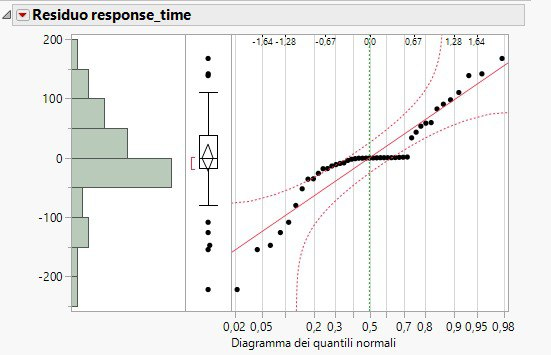
\includegraphics[width=0.8\textwidth]{img/ch3/qqplot_residui.png}
    \caption{Test di normalità dei residui}
    \label{fig:qqplot_residui}
\end{figure}


\paragraph{Omoschedasticità dei residui}
Come mostrato in \cref{fig:homo_residui}, la dispersione dei punti, per entrambi i fattori, dello \textit{scatter plot} non è costante, per cui è possibile rifiutare l’ipotesi di omoschedasticità degli errori. Oltre alla verifica visiva, è possibile affermare la non omoschedasticità dei residui attraverso il test di \textit{Levene}.

\begin{figure}[H]
    \centering
    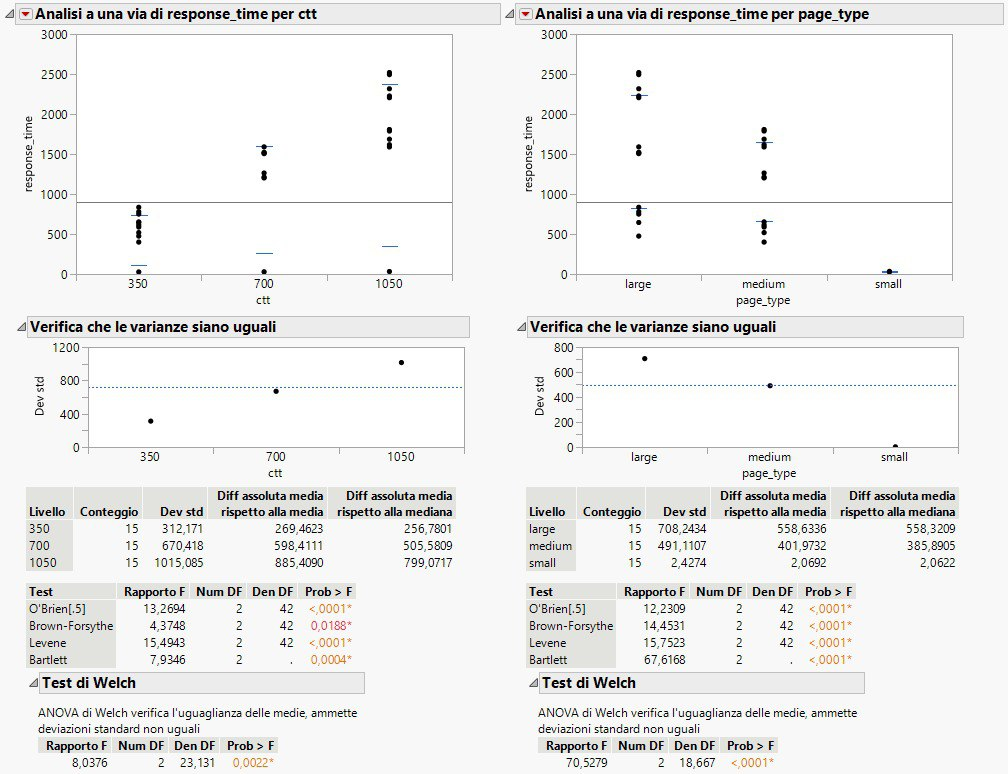
\includegraphics[width=\textwidth]{img/ch3/omoschedasticita_residui.png}
    \caption{Test di omoschedasticità dei residui}
    \label{fig:homo_residui}
\end{figure}


\paragraph{Test di significatività}

Dato che per entrambi i fattori risultano residui non normali e non omoschedastici, si è scelto di utilizzare il Test di \textit{Wilcoxon/Kruskal-Wallis}.

\begin{figure}[H]
    \centering
    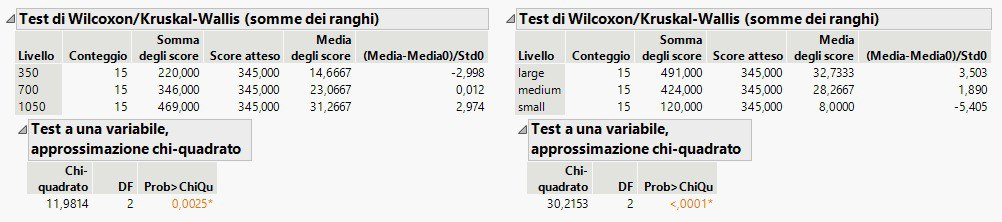
\includegraphics[width=\textwidth]{img/ch3/significativita.png}
    \caption{Test di significavità}
    \label{fig:significativita_fattori}
\end{figure}

Come mostrato in \cref{fig:significativita_fattori}, entrambi i fattori, \textit{Request Rate} e \textit{Page Size} risultano significativi a livello statistico.












\chapter{Regressione lineare}


\section{Exercise 1}
Rilevare e stimare eventuali trend su ognuna delle tre variabili nmail, byte rec e byte sent, utilizzando modelli regressivi lineari semplici, parametrici e/o non parametrici


La normalità dei residui è una condizione necessaria per l'utilizzo di una regressione lineare come modello, motivo per il quale per entrambi i dataset è stata inizialmente svolta un'analisi sulla normalità dei residui ottenuti in seguito a una stima lineare di ogni colonna rispetto alle osservazioni.


\subsection{EXP1}
È possibile notare dal diagramma quantile quantile e dal test di \textit{Anderson-Darling} la non normalità della distribuzione dei residui per tutte e tre le variabili (\cref{fig:4_ex1_traccia}).
Si è quindi proceduto con il test di \textit{Mann Kendall} per verificare la presenza di trend monotoni, e in caso positivo è stato calcolato lo \textit{slope} sia con la procedura di \textit{Theil-Sen}. Nei grafici che seguono è possibile notare in rosso i risultati ottenuti con \textit{Theil-Sen}, mentre in verde il risultato ottenuto con il metodo dei quadrati minimi, inserito come base di confronto.

\begin{figure}[H]
    \centering
    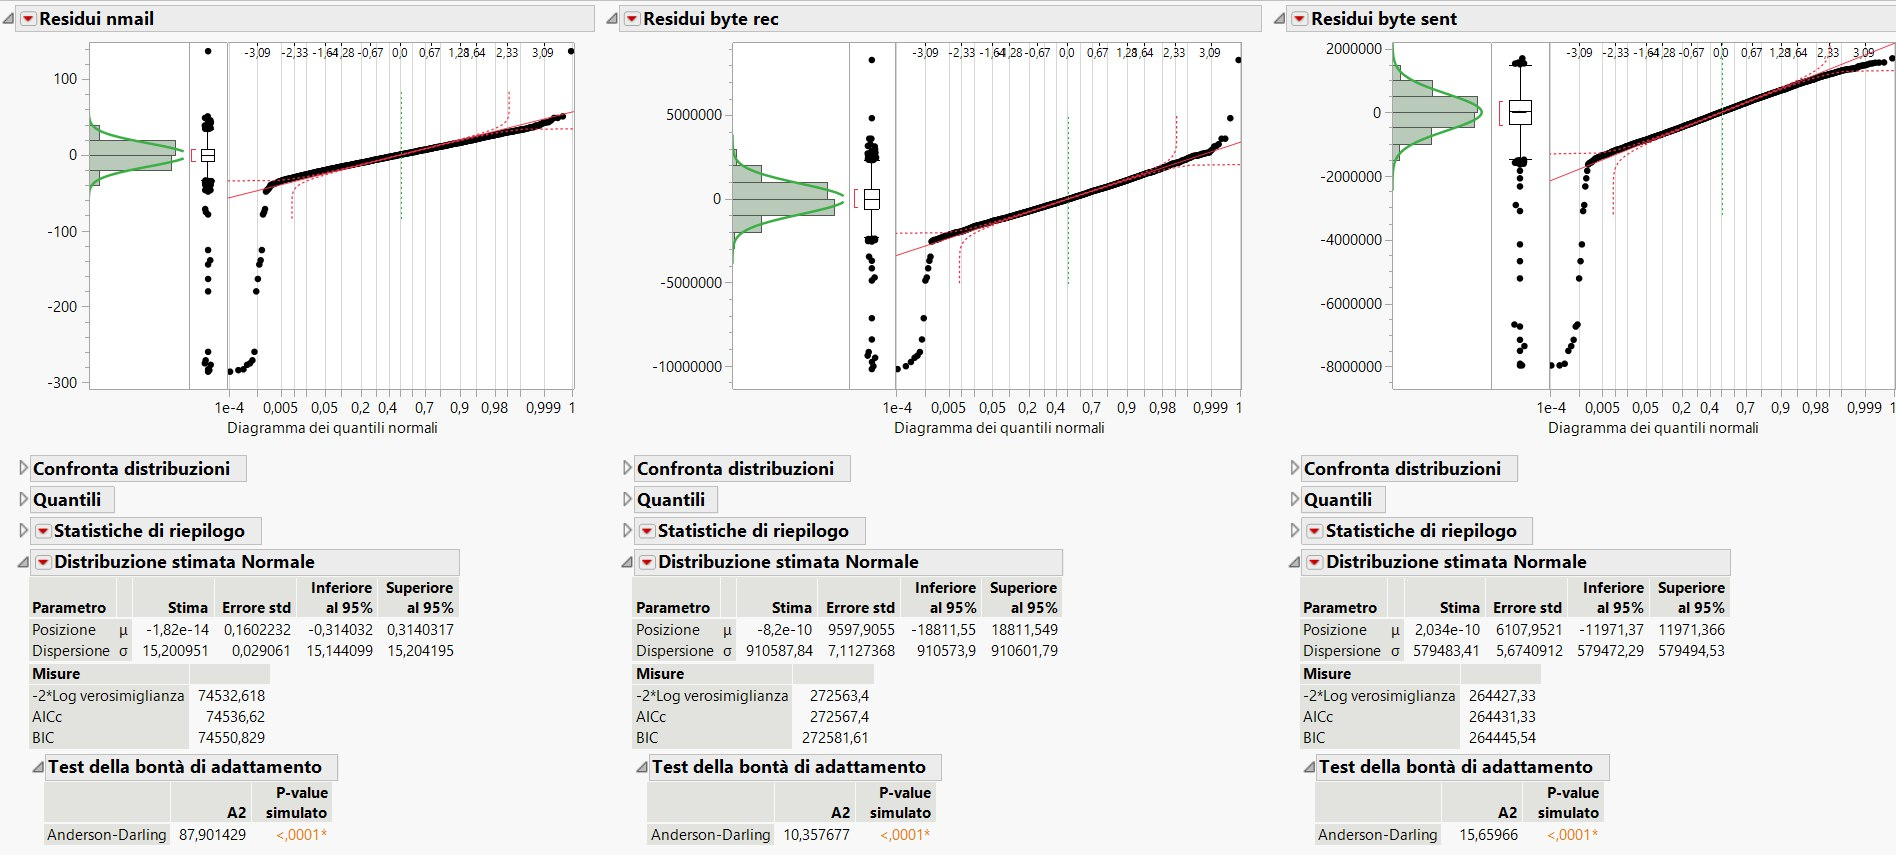
\includegraphics[width=\textwidth]{img/ch4/exp1norm.jpg}
    \caption{Test normalità residui}
    \label{fig:4_ex1_traccia}
\end{figure}

\paragraph{Analisi \textit{nmail}}
Il risultato del test di \textit{Man-Kendall} mostra che non è possibile determinare la presenza di un \textit{trend} ($pvalue=0.7163$). Si noti che l'intervallo di confidenza individuato con il test di Theil-Sen $(0.0;0.0)$ include il valore $0$. 

\begin{figure}[H]
    \centering
    \includegraphics[width=\textwidth]{img/ch4/exp1.1.pdf}
    \caption{Trend nmail per EXP1}
\end{figure}


\paragraph{Analisi \textit{byte rec}}
Il risultato del test di Man Kendall mostra che non è possibile determinare la presenza di un \textit{trend} ($pvalue=0.2001$). Si noti che l'intervallo di confidenza individuato con il test di Theil-Sen $(-11.5115;2.4138)$ include il valore $0$. 

\begin{figure}[H]
    \centering
    \includegraphics[width=\textwidth]{img/ch4/exp1.2.pdf}
    \caption{Trend byte rec}
    \label{fig:ex1_traccia}
\end{figure}


\paragraph{Analisi \textit{byte sent}}
Il risultato del test di Man Kendall mostra la presenza di un \textit{trend} decrescente ($pvalue=0.0434$). Il test di Theil-Sen produce una retta:

\begin{equation}
    y = -4.5147 \cdot x + 9959247.5279
\end{equation}

L'intervallo di confidenza (calcolato al $95\%$)  del coefficiente angolare è\\ $(-8.8910;-0.1306)$.

\begin{figure}[H]
    \centering
    \includegraphics[width=\textwidth]{img/ch4/exp1.3.pdf}
    \caption{Trend byte sent}
\end{figure}


\newpage
\subsection{EXP2}
Anche in questo caso è possibile notare dal diagramma quantile quantile e dal test di \textit{Anderson-Darlnig} la non normalità della distribuzione dei residui per tutte e tre le variabili (\cref{fig:4_ex2_traccia}).
Si è quindi proceduto con il test di \textit{Mann Kendall} per verificare la presenza di trend monotoni, e in caso positivo è stato calcolato lo slope con la procedura di \textit{Theil-Sen}.

\begin{figure}[H]
    \centering
    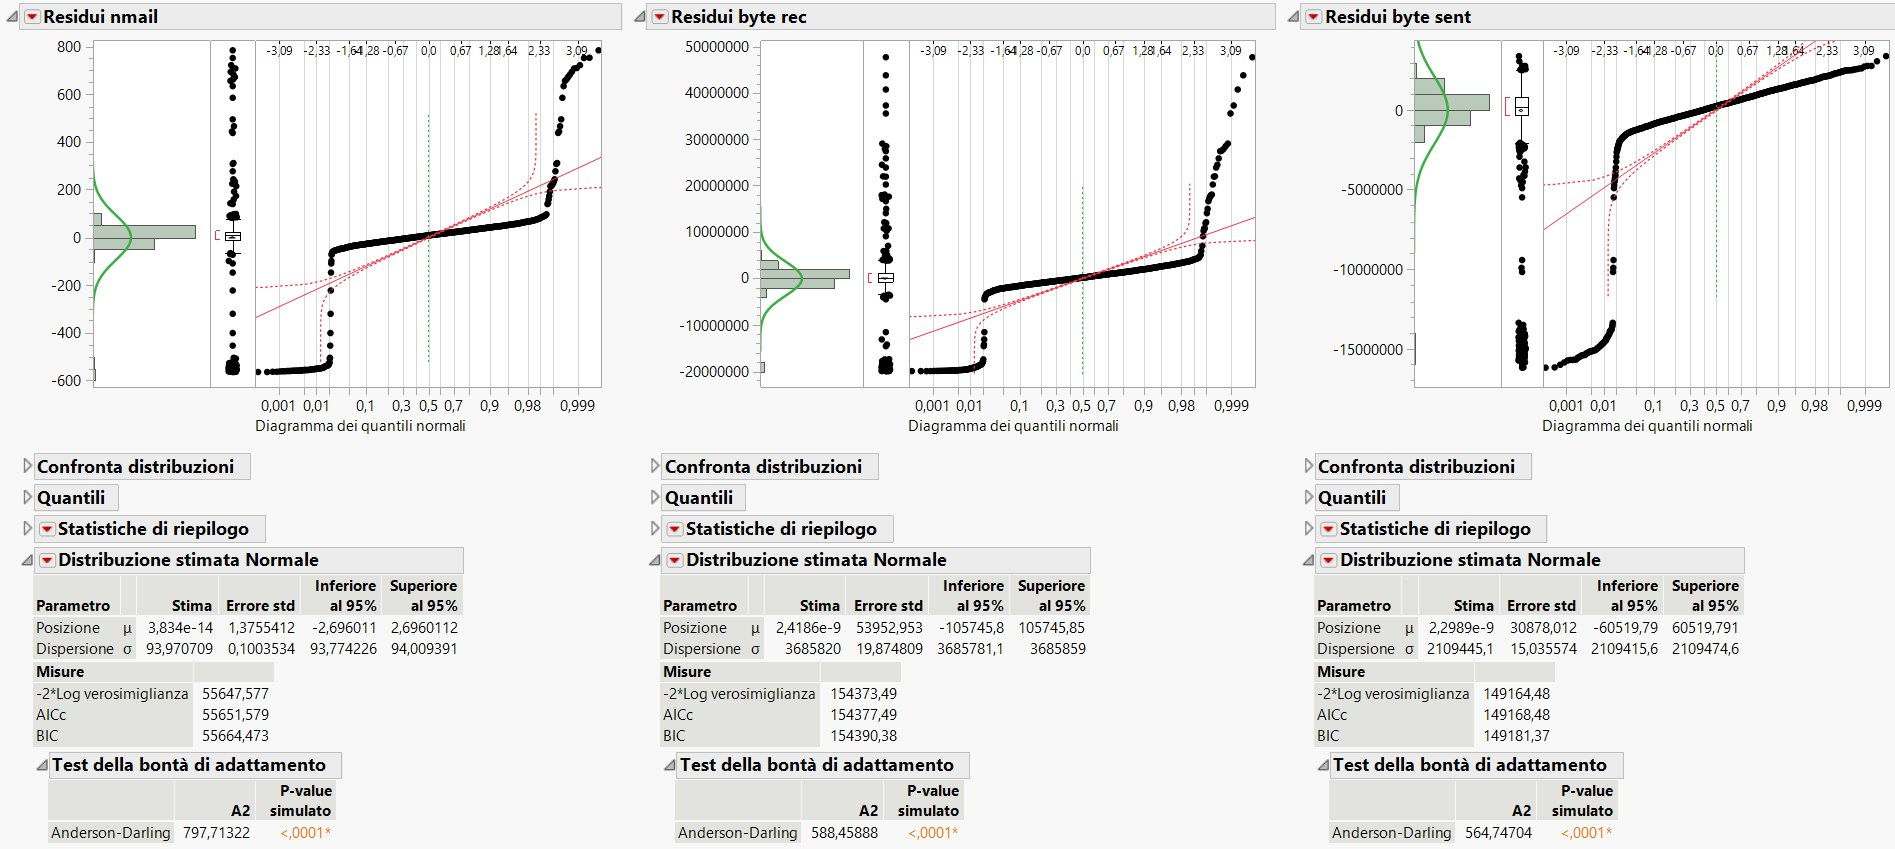
\includegraphics[width=\textwidth]{img/ch4/exp2.jpeg}
    \caption{Test normalità residui}
    \label{fig:4_ex2_traccia}
\end{figure}

\paragraph{Analisi \textit{nmail}}
Il risultato del test di Man Kendall mostra la presenza di un \textit{trend} decrescente ($pvalue=0.0138$). Il test di Theil-Sen produce una retta:

\begin{equation}
    y = -0.0005 x + 592.3936
\end{equation}

L'intervallo di confidenza (calcolato al $95\%$)  del coefficiente angolare è\\ $(-0.0011;0.0)$.

\begin{figure}[H]
    \centering
    \includegraphics[width=\textwidth]{img/ch4/exp2.1.pdf}
    \caption{Trend nmail per EXP2}
\end{figure}


\paragraph{Analisi \textit{byte rec}}
Il risultato del test di Man Kendall mostra la presenza di un \textit{trend} decrescente ($pvalue=0.0012$). Il test di Theil-Sen produce una retta:

\begin{equation}
    y = -48.2936 x + 20890131.9913
\end{equation}

L'intervallo di confidenza (calcolato al $95\%$) del coefficiente angolare è\\ $(-77.5477;-18.9931)$.

\begin{figure}[H]
    \centering
    \includegraphics[width=\textwidth]{img/ch4/exp2.2.pdf}
    \caption{Trend \textit{byte rec} EX1}
\end{figure}

\paragraph{Analisi \textit{byte sent}}
Il risultato del test di Man Kendall mostra la presenza di un \textit{trend} decrescente ($pvalue=5.8473\cdot 10^{-5}$). Il test di Theil-Sen produce una retta:
\begin{equation}
    y = -34.0630 x + 19903064.1005
\end{equation}

L'intervallo di confidenza (calcolato al $95\%$) del coefficiente angolare è\\ $(-50.6726;-17.3740)$.

\begin{figure}[H]
    \centering
    \includegraphics[width=\textwidth]{img/ch4/exp2.3.pdf}
    \caption{Trend \textit{byte sent} EX2}
\end{figure}

\newpage
\section{Exercise 2}
Rilevare e stimare eventuali trend sulle 5 variabili utilizzando modelli regressivi lineari semplici, parametrici e/o non parametrici. Farlo per i tre dataset os1, os2 e os3.
Confrontare i trend individuati nei tre dataset.

Per tutti e tre i dataset è stata inizialmente svolta un'analisi sulla normalità dei residui ottenuti in seguito a una stima lineare di ogni colonna rispetto al tempo di osservazione. 

\subsection{Sistema \textit{os1}}
È possibile notare dal diagramma quantile quantile e dal test di \textit{Anderson-Darling} la non normalità delle distribuzioni (\cref{fig:4_os1_traccia}).
Si è quindi proceduto con il test di \textit{Mann Kendall} per verificare la presenza di trend monotoni, e in caso positivo è stato calcolato lo slope con la procedura di \textit{Theil-Sen}.

\begin{figure}[H]
    \centering
    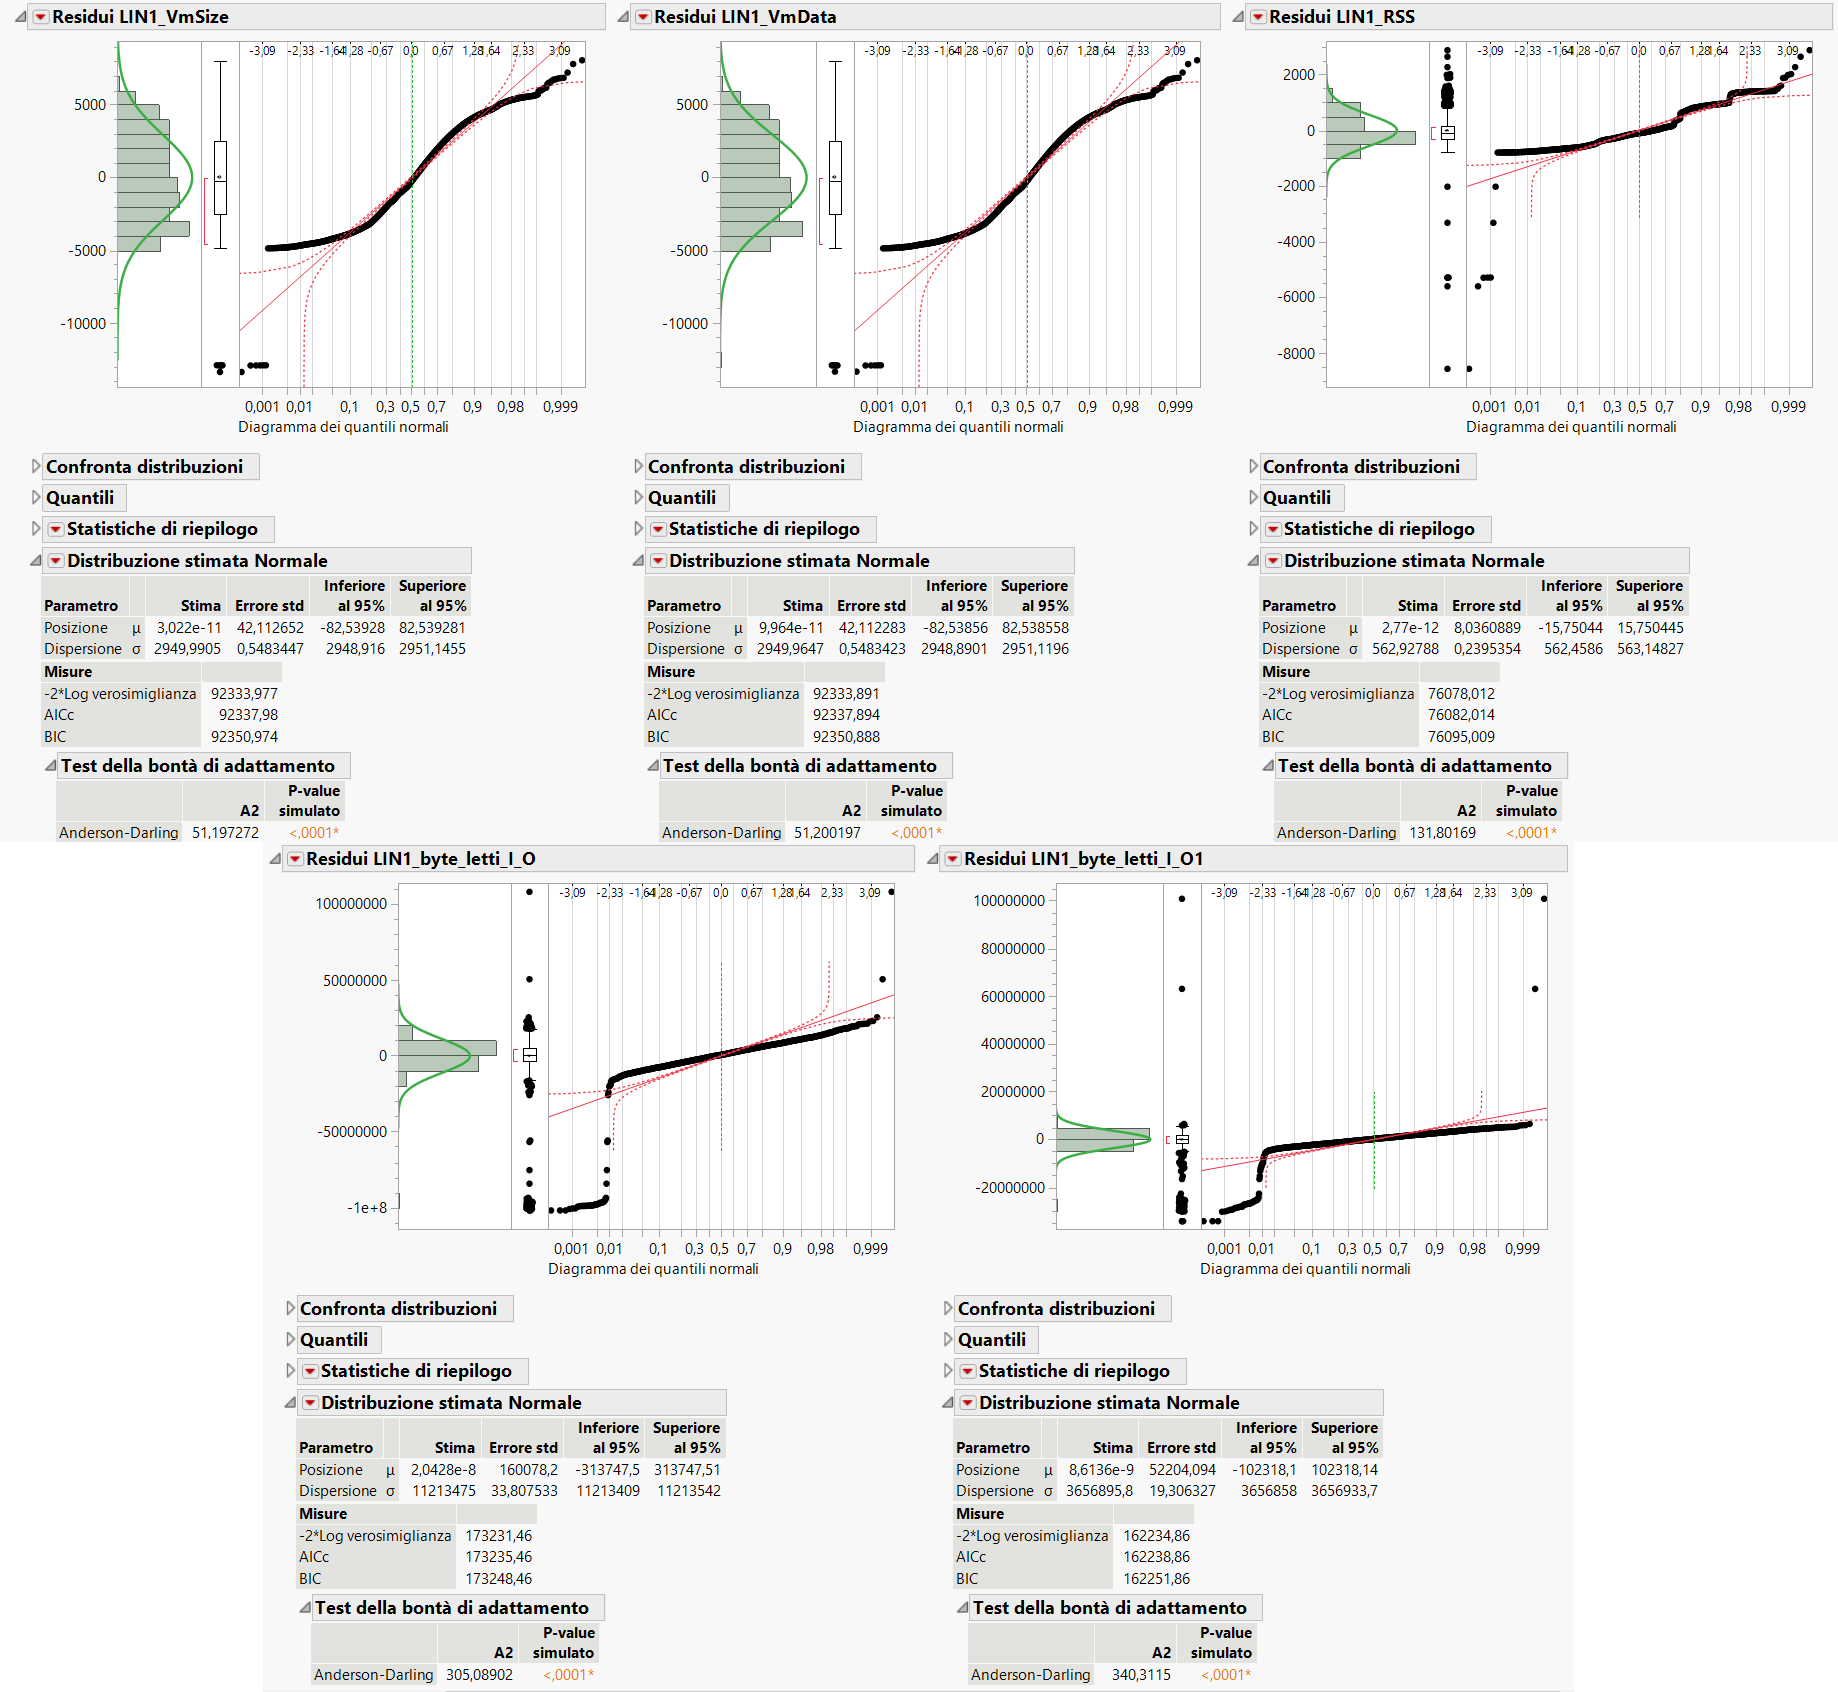
\includegraphics[width=\textwidth]{img/ch4/os1norm.png}
    \caption{Test normalità residui per $os1$}
    \label{fig:4_os1_traccia}
\end{figure}

\paragraph{LIN1 VmSize}
Il risultato del test di Man Kendall mostra la presenza di un \textit{trend} crescente ($pvalue=0.0$). Il test di Theil-Sen produce una retta:
\begin{equation}
    y = 0.03151 x + 738854.3947
\end{equation}

L'intervallo di confidenza (calcolato al $95\%$) del coefficiente angolare è\\ $(0.0307;0.0323)$.

\begin{figure}[H]
    \centering
    \includegraphics[width=\textwidth]{img/ch4/os1.1.pdf}
    \caption{Trend LIN1 VmSize}
\end{figure}

\paragraph{LIN1 VmData}
Il risultato del test di Man Kendall mostra la presenza di un \textit{trend} crescente ($pvalue=0.0$). Il test di Theil-Sen produce una retta:
\begin{equation}
    y = 0.0315 x + 670450.3948
\end{equation}

L'intervallo di confidenza (calcolato al $95\%$) del coefficiente angolare è\\ $(0.0307;0.0323)$.

\begin{figure}[H]
    \centering
    \includegraphics[width=\textwidth]{img/ch4/os1.2.pdf}
    \caption{Trend LIN1 VmData}
\end{figure}

\paragraph{LIN1 RSS}
Il risultato del test di Man Kendall mostra la presenza di un \textit{trend} crescente ($pvalue=0.0$). Il test di Theil-Sen produce una retta:
\begin{equation}
    y = 0.0049 x + 42428.8070
\end{equation}

L'intervallo di confidenza (calcolato al $95\%$) del coefficiente angolare è\\ $(0.00488;0.0050)$.

\begin{figure}[H]
    \centering
    \includegraphics[width=\textwidth]{img/ch4/os1.3.pdf}
    \caption{Trend LIN1 RSS}
\end{figure}

\paragraph{LIN1 byte letti IO}
Il risultato del test di Man Kendall mostra la presenza di un \textit{trend} crescente ($pvalue=0.0$). Il test di Theil-Sen produce una retta:
\begin{equation}
    y = 4.7375 x + 102763229.5031
\end{equation}

L'intervallo di confidenza (calcolato al $95\%$) del coefficiente angolare è\\ $(3.6739;5.8045)$.


\begin{figure}[H]
    \centering
    \includegraphics[width=\textwidth]{img/ch4/os1.4.pdf}
    \caption{Trend LIN1 byte letti I O}
\end{figure}

\paragraph{LIN1 byte letti IO1}
Il risultato del test di Man Kendall mostra che non è possibile determinare la presenza di un \textit{trend} ($pvalue=0.8554$). Si noti che l'intervallo di confidenza individuato con il test di Theil-Sen $(-0.3608;0.2984)$ include il valore $0$. 


\begin{figure}[H]
    \centering
    \includegraphics[width=\textwidth]{img/ch4/os1.5.pdf}
    \caption{Trend LIN1 byte letti I O1}
\end{figure}


\newpage
\subsection{os2}
È possibile notare dal diagramma quantile quantile e dal test di \textit{Anderson-Darlnig} la non normalità delle distribuzione dei residui per le cinque variabili (\cref{fig:4_os2_traccia}).
Si è quindi proceduto con il test di \textit{Mann Kendall} per verificare la presenza di trend monotoni, e in caso positivo è stato calcolato lo slope con la procedura di \textit{Theil-Sen}.

\begin{figure}[H]
    \centering
    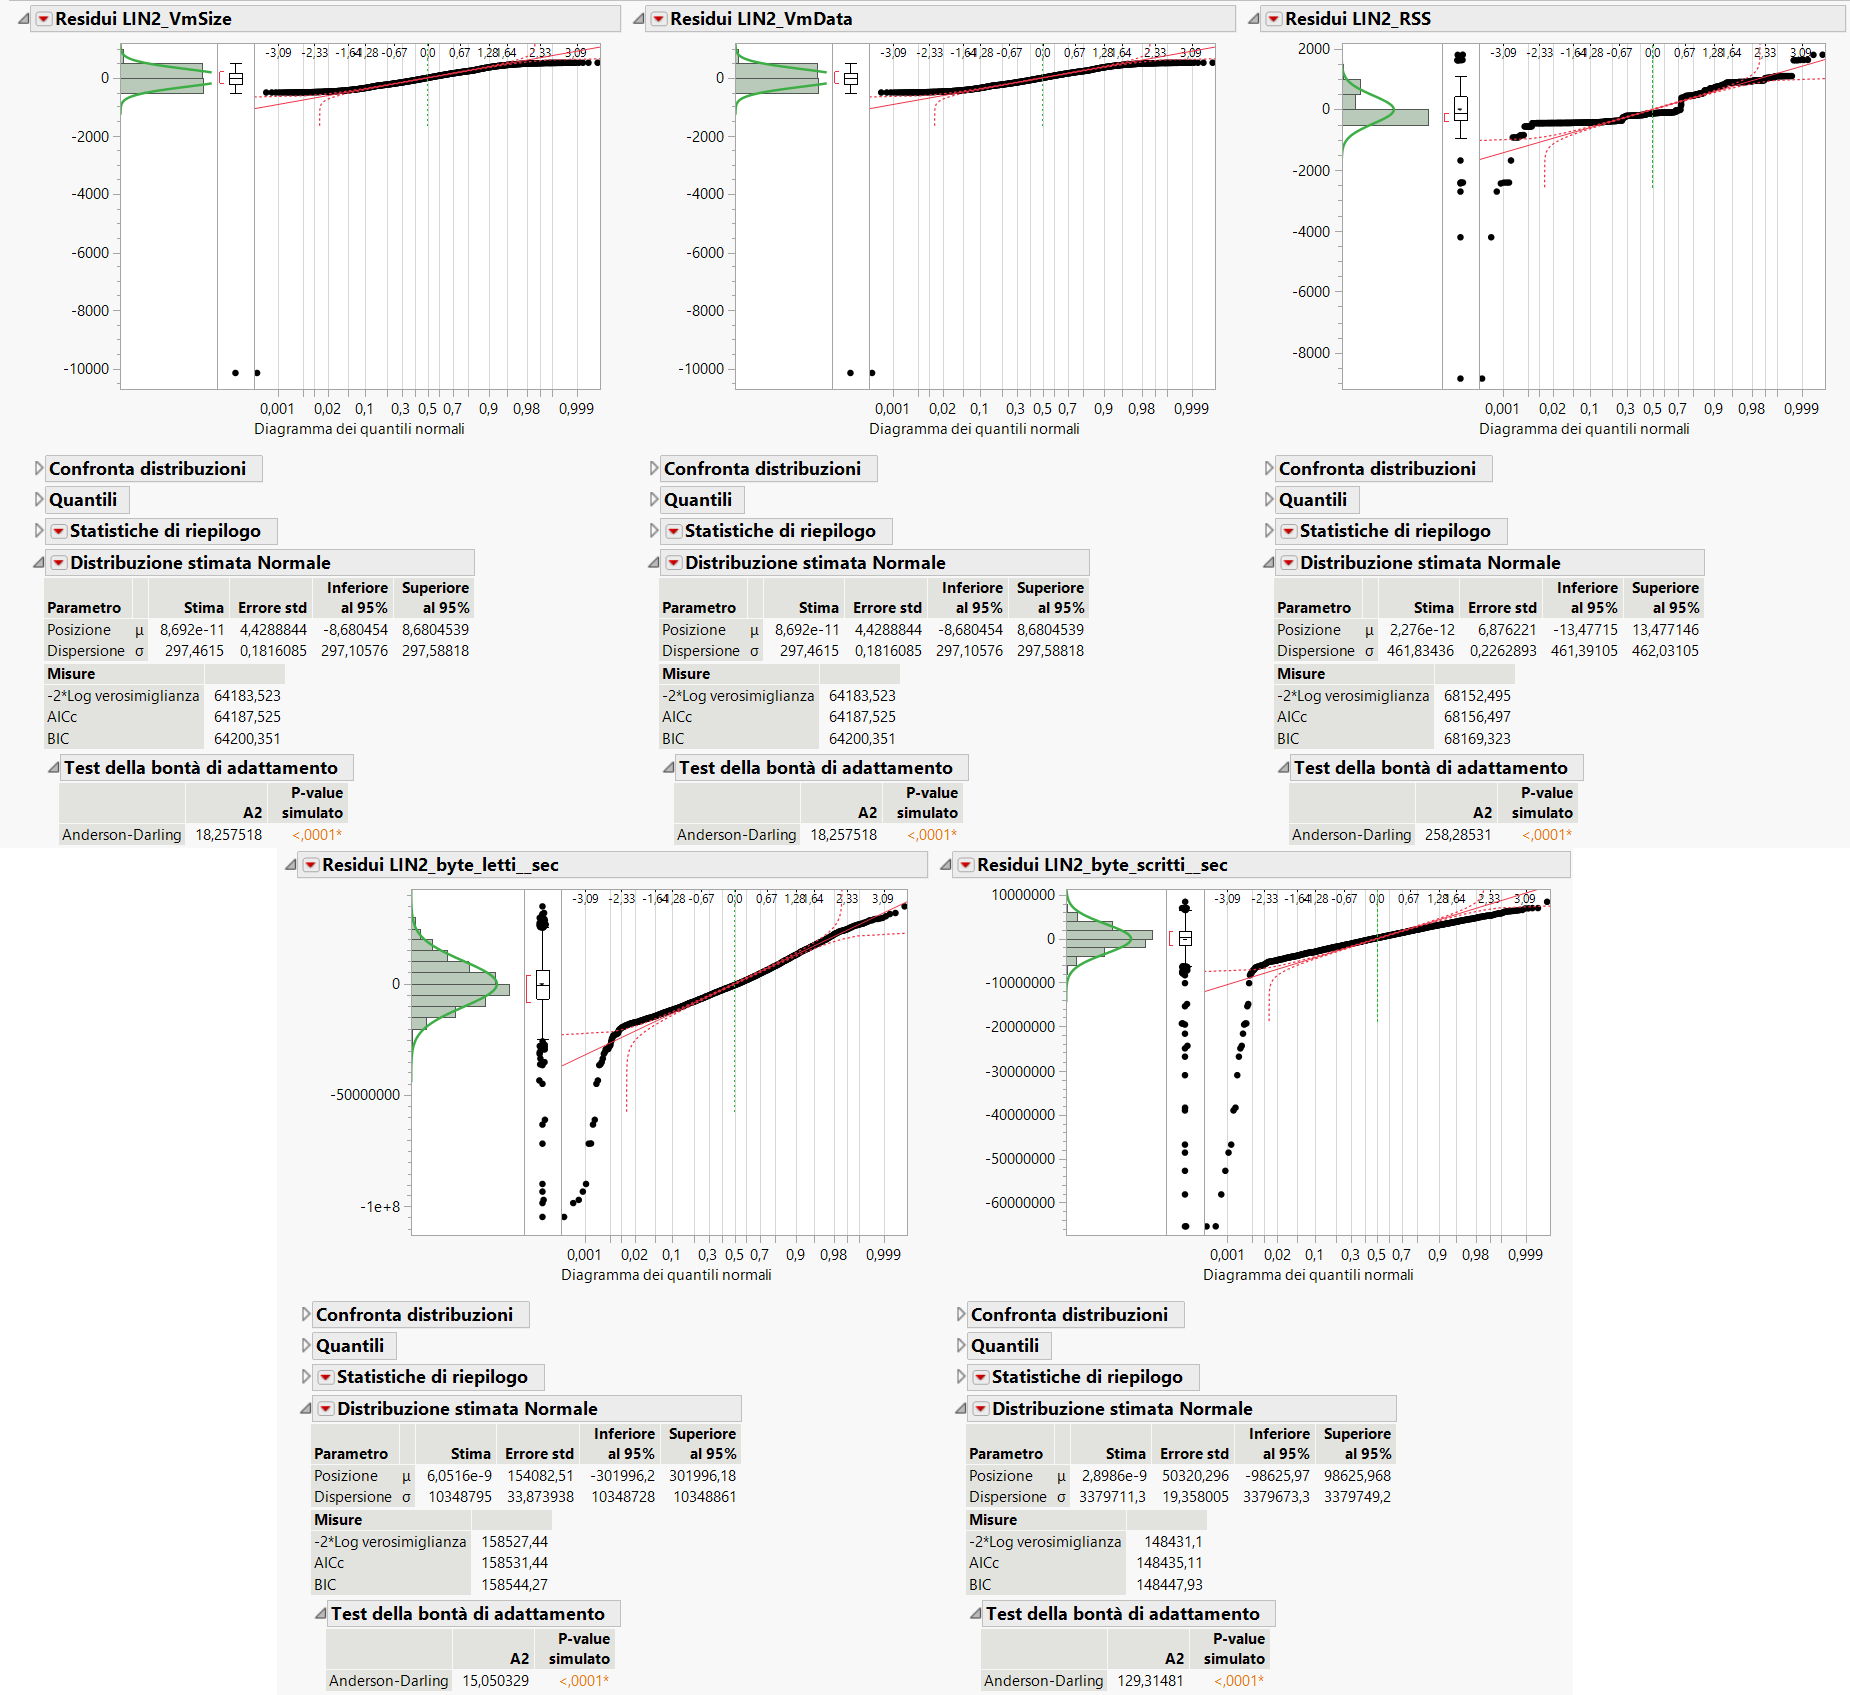
\includegraphics[width=\textwidth]{img/ch4/os2norm.png}
    \caption{Test normalità residui}
    \label{fig:4_os2_traccia}
\end{figure}

\paragraph{LIN2 VmSize}
Il risultato del test di Man Kendall mostra la presenza di un \textit{trend} crescente ($pvalue=0.0$). Il test di Theil-Sen produce una retta:
\begin{equation}
    y = 0.0019 x + 735790.3761
\end{equation}

L'intervallo di confidenza (calcolato al $95\%$) del coefficiente angolare è\\ $(0.0;0.0020)$.


\begin{figure}[H]
    \centering
    \includegraphics[width=\textwidth]{img/ch4/os2.1.pdf}
    \caption{Trend LIN2 VmSize}
\end{figure}

\paragraph{LIN2 VmData}
Il risultato del test di Man Kendall mostra la presenza di un \textit{trend} crescente ($pvalue=0.0$). Il test di Theil-Sen produce una retta:
\begin{equation}
    y = 0.0019 x + 667414.3761
\end{equation}

L'intervallo di confidenza (calcolato al $95\%$) del coefficiente angolare è\\ $(0.0;0.0020)$.

\begin{figure}[H]
    \centering
    \includegraphics[width=\textwidth]{img/ch4/os2.2.pdf}
    \caption{Trend LIN2 VmData}
\end{figure}

\paragraph{LIN2 RSS}
Il risultato del test di Man Kendall mostra la presenza di un \textit{trend} crescente ($pvalue=0.0$). Il test di Theil-Sen produce una retta:
\begin{equation}
    y = 0.0006x + 42384.8545
\end{equation}

L'intervallo di confidenza (calcolato al $95\%$) del coefficiente angolare è\\ $(0.0005;0.0007)$.

\begin{figure}[H]
    \centering
    \includegraphics[width=\textwidth]{img/ch4/os2.3.pdf}
    \caption{Trend LIN2 RSS}
\end{figure}

\paragraph{LIN2 byte letti sec}
Il risultato del test di Man Kendall mostra la presenza di un \textit{trend} crescente ($pvalue=0.0$). Il test di Theil-Sen produce una retta:
\begin{equation}
    y = 114.5535 x + 77733384.2378
\end{equation}

L'intervallo di confidenza (calcolato al $95\%$) del coefficiente angolare è\\ $(112.7335;116.3765)$.


\begin{figure}[H]
    \centering
    \includegraphics[width=\textwidth]{img/ch4/os2.4.pdf}
    \caption{Trend LIN2  byte letti sec}
\end{figure}

\paragraph{LIN2 byte scritti sec}
Il risultato del test di Man Kendall mostra la presenza di un \textit{trend} decrescente ($pvalue=0.0$). Il test di Theil-Sen produce una retta:
\begin{equation}
    y = -0.4886 x + 65693615.5762
\end{equation}

L'intervallo di confidenza (calcolato al $95\%$) del coefficiente angolare è\\ $(-0.9390;-0.0363)$.

\begin{figure}[H]
    \centering
    \includegraphics[width=\textwidth]{img/ch4/os2.5.pdf}
    \caption{LIN2 byte scritti sec}
\end{figure}

\newpage
\subsection{os3}

è possibile notare dal diagramma quantile quantile e dal test di \textit{Anderson-Darlnig} la non normalità delle distribuzioni (\cref{fig:4_os3_traccia}).
Si è quindi proceduto con il test di \textit{Mann Kendall} per verificare la presenza di trend monotoni, e in caso positivo è stato calcolato lo slope con la procedura di \textit{Theil-Sen}.

\begin{figure}[H]
    \centering
    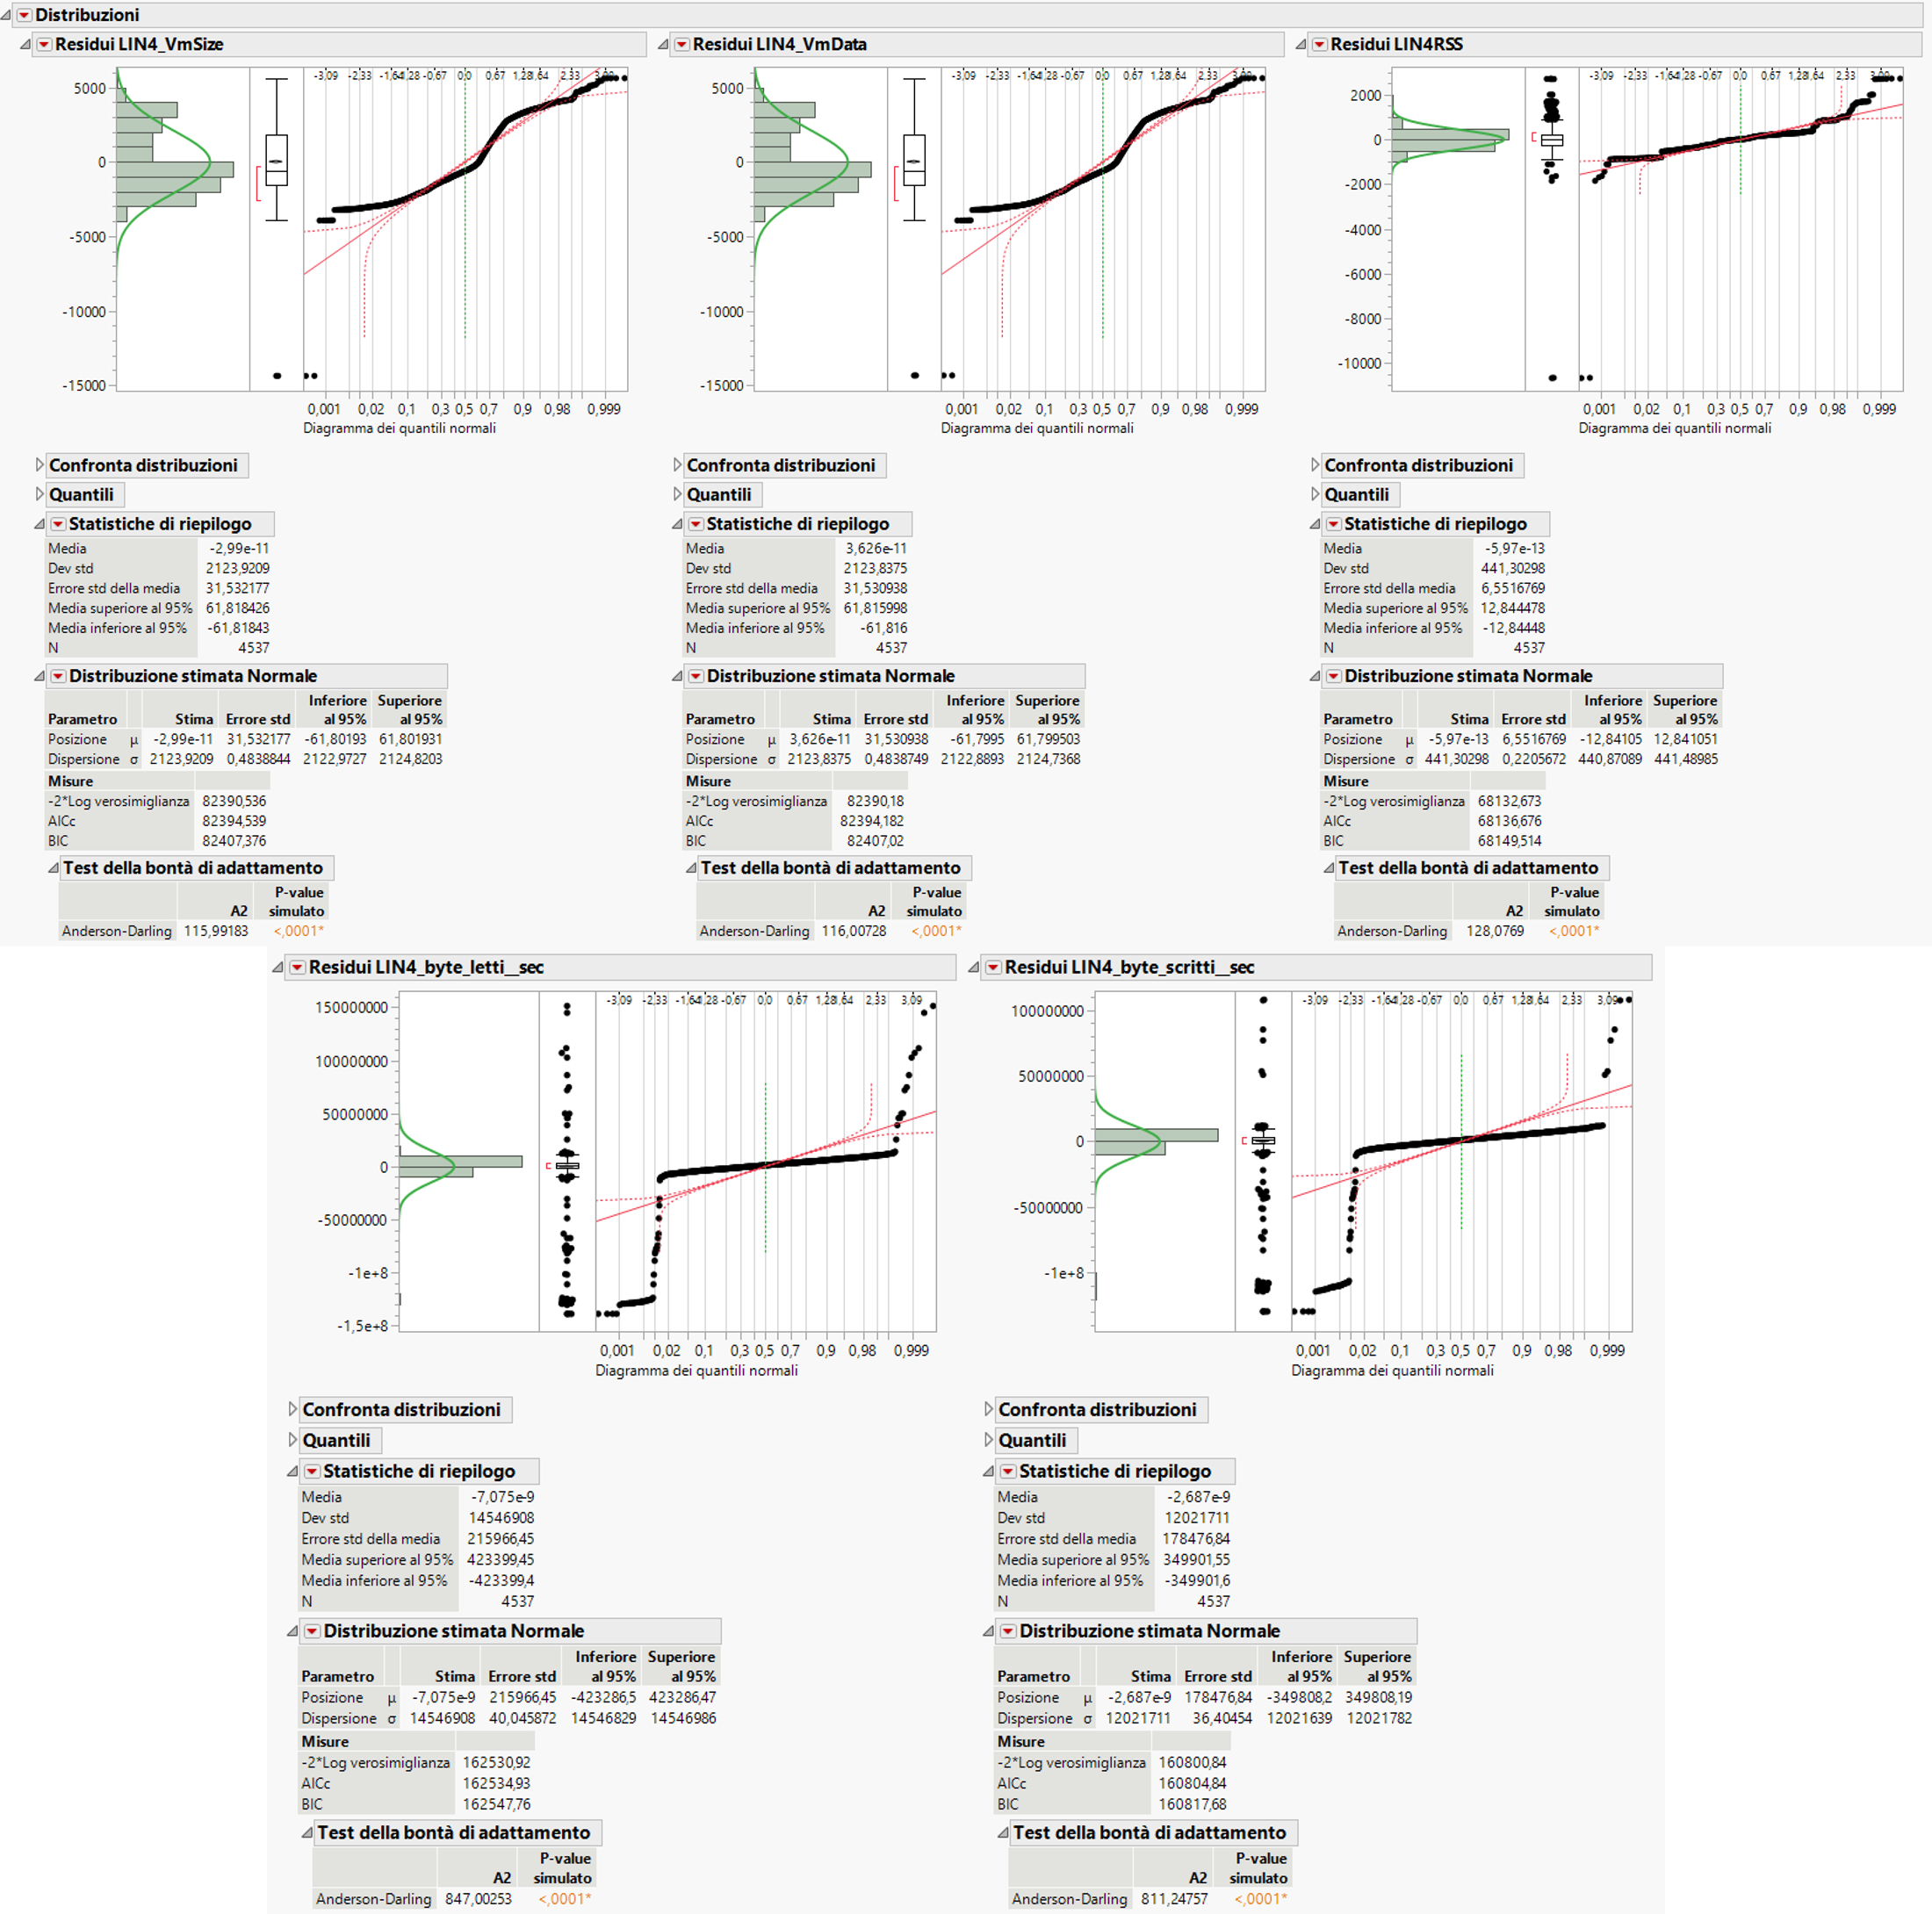
\includegraphics[width=\textwidth]{img/ch4/os3_norm.png}
    \caption{Test normalità residui}
    \label{fig:4_os3_traccia}
\end{figure}

\paragraph{LIN4 VmSize}
Il risultato del test di Man Kendall mostra la presenza di un \textit{trend} crescente ($pvalue=0.0$). Il test di Theil-Sen produce una retta:
\begin{equation}
    y = 0.0216 x + 744373.4861
\end{equation}

L'intervallo di confidenza (calcolato al $95\%$) del coefficiente angolare è\\ $(0.0212;0.0220)$.

\begin{figure}[H]
    \centering
    \includegraphics[width=\textwidth]{img/ch4/os3.1.pdf}
    \caption{LIN4 VmSize}
\end{figure}

\paragraph{LIN4 VmData}
Il risultato del test di Man Kendall mostra la presenza di un \textit{trend} crescente ($pvalue=0.0$). Il test di Theil-Sen produce una retta:
\begin{equation}
    y = 0.0217 x + 675969.4861
\end{equation}

L'intervallo di confidenza (calcolato al $95\%$) del coefficiente angolare è\\ $(0.0212;0.0220)$.

\begin{figure}[H]
    \centering
    \includegraphics[width=\textwidth]{img/ch4/os3.2.pdf}
    \caption{Trend LIN4 VmData}
    \label{fig:ex1_traccia}
\end{figure}

\paragraph{LIN4 RSS}
Il risultato del test di Man Kendall mostra la presenza di un \textit{trend} crescente ($pvalue=0.0$). Il test di Theil-Sen produce una retta:
\begin{equation}
    y = 0.0034 x + 45386.0844
\end{equation}

L'intervallo di confidenza (calcolato al $95\%$) del coefficiente angolare è\\ $(0.0033;0.0035)$.

\begin{figure}[H]
    \centering
    \includegraphics[width=\textwidth]{img/ch4/os3.3.pdf}
    \caption{Trend LIN4 RSS}
\end{figure}

\paragraph{LIN4 byte letti sec}
Il risultato del test di Man Kendall mostra la presenza di un \textit{trend} decrescente ($pvalue=1.0286 \cdot 10^{-7}$). Il test di Theil-Sen produce una retta:
\begin{equation}
    y = -1.9637 x + 141319342.3890
\end{equation}

L'intervallo di confidenza (calcolato al $95\%$) del coefficiente angolare è\\ $(-2.6876;-1.2433)$.

\begin{figure}[H]
    \centering
    \includegraphics[width=\textwidth]{img/ch4/os3.4.pdf}
    \caption{Trend LIN4 byte letti sec}
\end{figure}

\paragraph{LIN4 byte scritti sec}
Il risultato del test di Man Kendall mostra che non è possibile determinare la presenza di un \textit{trend} ($pvalue=0.0539$). Si noti che l'intervallo di confidenza individuato con il test di Theil-Sen $(-1.2588;0.0104)$ include il valore $0$. 


\begin{figure}[H]
    \centering
    \includegraphics[width=\textwidth]{img/ch4/os3.5.pdf}
    \caption{LIN4 byte scritti sec}
\end{figure}

\newpage
\subsection{Confronto tra i sistemi}

\begin{figure}[H]
    \centering
    \includegraphics[width=\textwidth]{img/ch4/os_comp.pdf}
    \caption{Confronto tra \textit{os1}, \textit{os2}, \textit{os3}}
\end{figure}


\begin{itemize}
    \item Memoria Virtuale: dai grafici, si osserva che VMsize e VMdata sono correlati strettamente tra loro , e che in \textit{os1} e \textit{os3} sono presenti trend monotoni crescenti più accentuati, mentre per \textit{os2} c'è sempre un trend crescente ma più lento.
    \item RSS: anche in questo caso tutti i sistemi presentano dei trend monotoni crescenti, con \textit{os2} meno accentuato.
    \item Byte letti: dai risultati ottenuti è possibile notare un trend monotono crescente accentuato su \textit{os2}, mentre per \textit{os1} e \textit{os3}, sono presenti rispettivamente un trend crescente e uno decrescente, entrambi di lieve entità.
    \item Byte scritti: per \textit{os1} e \textit{os3} non è stato rilevato alcun trend, e per os2 esiste un trend monotono decrescente poco accentuato.
\end{itemize}

\newpage
\section{Exercise 3}
Supponendo di avere un limite massimo alla memoria heap di 1 GByte. Rilevare un eventuale trend di consumo dello heap nell'esperimento in figura. Se rilevato il trend, stimare il tempo  in cui lo heap satura (failure prediction).

\subsection{VMres1}
La \cref{fig:4_vmres1_traccia} mostra la non normalità dei residui. Quindi si è proceduto con l'applicazione dei test non parametrici quali \textit{Man-Kendall} per il rilevamento di trend e di \textit{Theil-Sen} per il calcolo dei parametri della retta regressiva.
\begin{figure}[H]
    \centering
    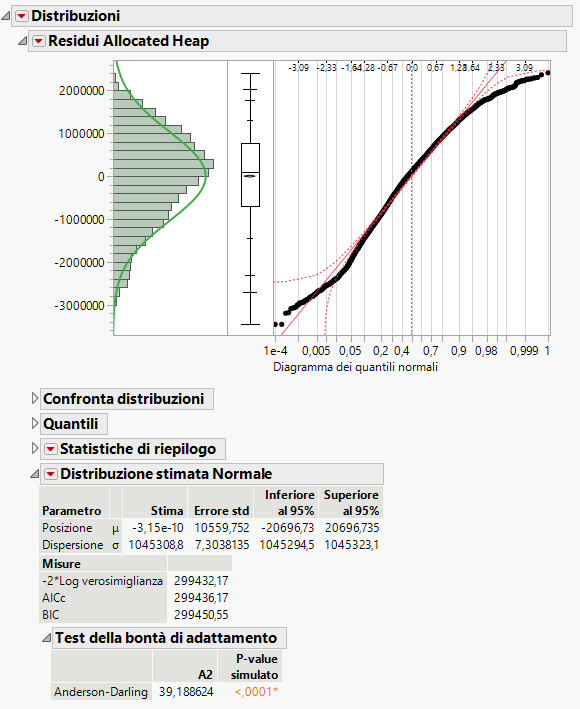
\includegraphics[width=\textwidth]{img/ch4/vm1_norm.png}
    \caption{Normalità residui VMres1}
    \label{fig:4_vmres1_traccia}
\end{figure}


\paragraph{Allocated Heap}
Il risultato del test di Man Kendall mostra la presenza di un \textit{trend} crescente ($pvalue=0.0$). Il test di Theil-Sen produce una retta:
\begin{equation}
    y = 0.6911 x + 6562275.4616
\end{equation}

L'intervallo di confidenza (calcolato al $95\%$) del coefficiente angolare è\\ $(0.5637;0.8178)$.

\begin{figure}[H]
    \centering
    \includegraphics[width=\textwidth]{img/ch4/vmres1.1.pdf}
    \caption{Trend Allocated Heap}
\end{figure}

\subsection{VMres2}
Analogamente a \textit{VMRes1}, anche i residui di \textit{VMRes2} non seguono una distribuione normale (\cref{fig:4_vmres2_traccia}). Pertanto, si è proceduto con l'applicazione di test non parametrici.
\begin{figure}[H]
    \centering
    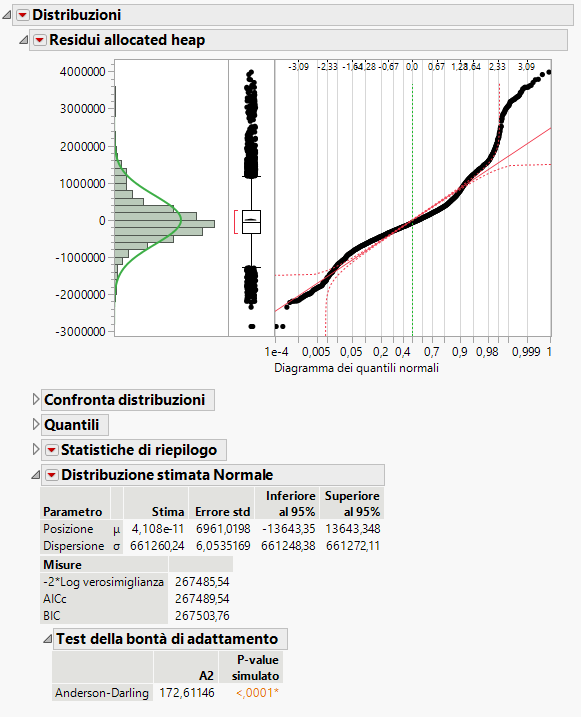
\includegraphics[width=\textwidth]{img/ch4/vm2_norm.png}
    \caption{Normalità residui VMres2}
     \label{fig:4_vmres2_traccia}
\end{figure}

\paragraph{Allocated Heap}

Il risultato del test di Man Kendall mostra la presenza di un \textit{trend} crescente ($pvalue=1.0286 \cdot 10^{-7}$). Il test di Theil-Sen produce una retta:
\begin{equation}
    y = 0.6709 x + 5780180.5633
\end{equation}

L'intervallo di confidenza (calcolato al $95\%$) del coefficiente angolare è\\ $(0.6048;0.7366)$.

\begin{figure}[H]
    \centering
    \includegraphics[width=\textwidth]{img/ch4/vmres2.1.pdf}
    \caption{Trend Allocated Heap}
\end{figure}

\subsection{VMres3}
Infine, anche i residui di \textit{VMRes3} non seguono la distribuzione normale (\cref{fig:4_vmres3_traccia}). Quindi, si è applicato il test \textit{Man-Kendall} per il rilevamento dei \textit{trend}.

\begin{figure}[H]
    \centering
    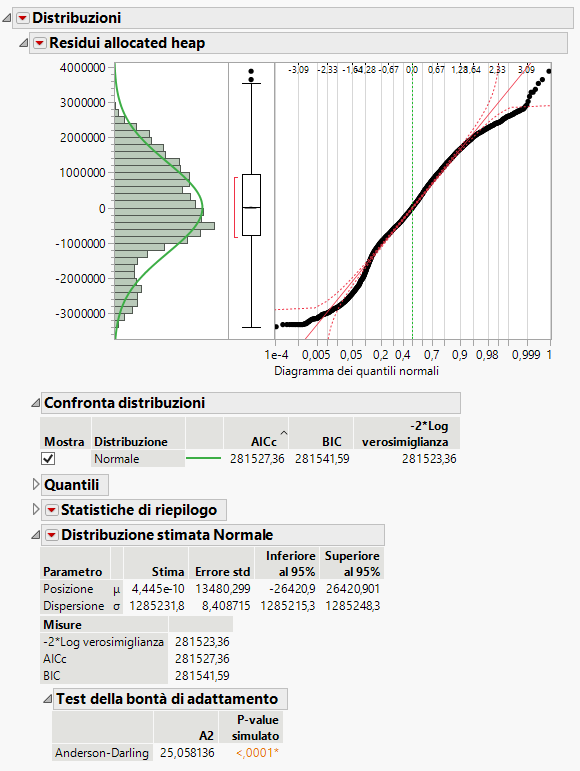
\includegraphics[width=\textwidth]{img/ch4/vm3_norm.png}
    \caption{Normalità residui VMres3}
     \label{fig:4_vmres3_traccia}
\end{figure}

\paragraph{Allocated Heap}

Il risultato del test di Man Kendall mostra la presenza di un \textit{trend} crescente ($pvalue=1.0286 \cdot 10^{-7}$). Il test di Theil-Sen produce una retta:
\begin{equation}
    y = 2.9030 x + 6041585.5564
\end{equation}

L'intervallo di confidenza (calcolato al $95\%$) del coefficiente angolare è\\ $(2.7147;3.0923)$.

\begin{figure}[H]
    \centering
    \includegraphics[width=\textwidth]{img/ch4/vmres3.1.pdf}
    \caption{Trend Allocated Heap}
\end{figure}

\clearpage
\subsection{Failure prediction} 

Dai risultati precedenti è possibile ottenere le rette di regressione relative ai 3 sistemi (riportate in \cref{eq:vm1_regression}, \cref{eq:vm2_regression}, \cref{eq:vm3_regression}), all'interno delle quali basterà imporre $Allocated\_Heap = 1000000000$ per trovare il tempo di saturazione a $1GB$.

\begin{align}
    \label{eq:vm1_regression}
    Allocated\_Heap_1 = 0.6911 \cdot T(s) +6562275.4616 \\ 
    \label{eq:vm2_regression}
    Allocated\_Heap_2 = 0.6709 \cdot T(s) +5780180.5633 \\
    \label{eq:vm3_regression}
    Allocated\_Heap_3 = 2.9030 \cdot T(s) +6041585.5564
\end{align}

Quindi sostituendo i valori numerici, si ottengono i seguenti tempi di saturazione:
\begin{itemize}
    \item VMres1: $ T \approx 45,6 $ anni 
    \item VMres2: $ T \approx 46,9 $ anni
    \item VMres3: $ T \approx 10,8 $ anni
\end{itemize}










\chapter{RBD}

\section{Exercise 1}
 Find the $R(t)$ and $MMTF$ for the system whose reliability diagram is given below. In calculating $MTTF$, assume all components are identical and fail randomly with failure rate $\lambda$.

\begin{figure}[h]
    \centering
    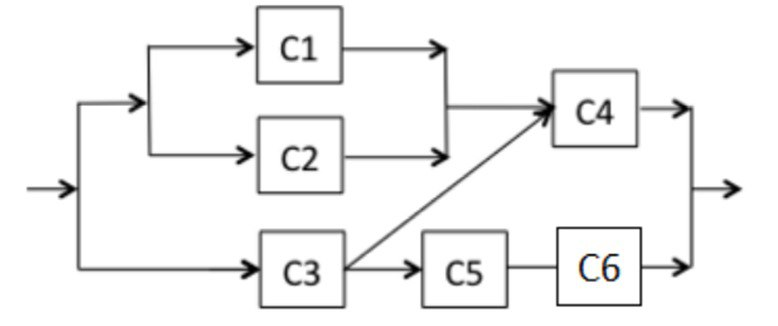
\includegraphics[width=0.8\textwidth]{img/ch5/ex1_traccia.png}
    \caption{RBD esercizio 1}
    \label{fig:ex1_traccia}
\end{figure}

Dallo schema in \cref{fig:ex1_traccia}, si osserva che il sistema non può essere ridotto ad un insieme di serie e parallelo a causa del collegmaento $C_3 \rightarrow C_4$. Pertanto, si è deciso procedere prima con la tecnica dell'\textit{upper bound} (\cref{eq:upper_bound_noserie_nopara}, dove con $R_{path}^i$ si indica la \textit{reliability} dell'i-esimo \textit{path} costituito dei componenti in serie del sistema.) e poi con quella del \textit{conditioning}.

\newpage
\subsection{Upper bound}
Applicando la formula in \cref{eq:upper_bound_noserie_nopara}:

\begin{equation}
    R_{sys} \leq 1 -\prod{(1 - R_{path}^i}) \
    \label{eq:upper_bound_noserie_nopara}
\end{equation}
, si calcola il limite superiore della reliability del sistema dato:

\begin{equation*}
    R_{sys} \leq 1 - [(1-R_1R_4) (1-R_2R_4) (1-R_2R_4) (1-R_3R_5R_6)]
\end{equation*}

Sostituendo i dati del problema si ottiene:

\begin{equation*}
    R_{sys} \leq 1 - [(1 - e^{-3 \lambda t}) (1 - e^{-2 \lambda t})^3]
\end{equation*}


\begin{figure}[H]
    \centering
    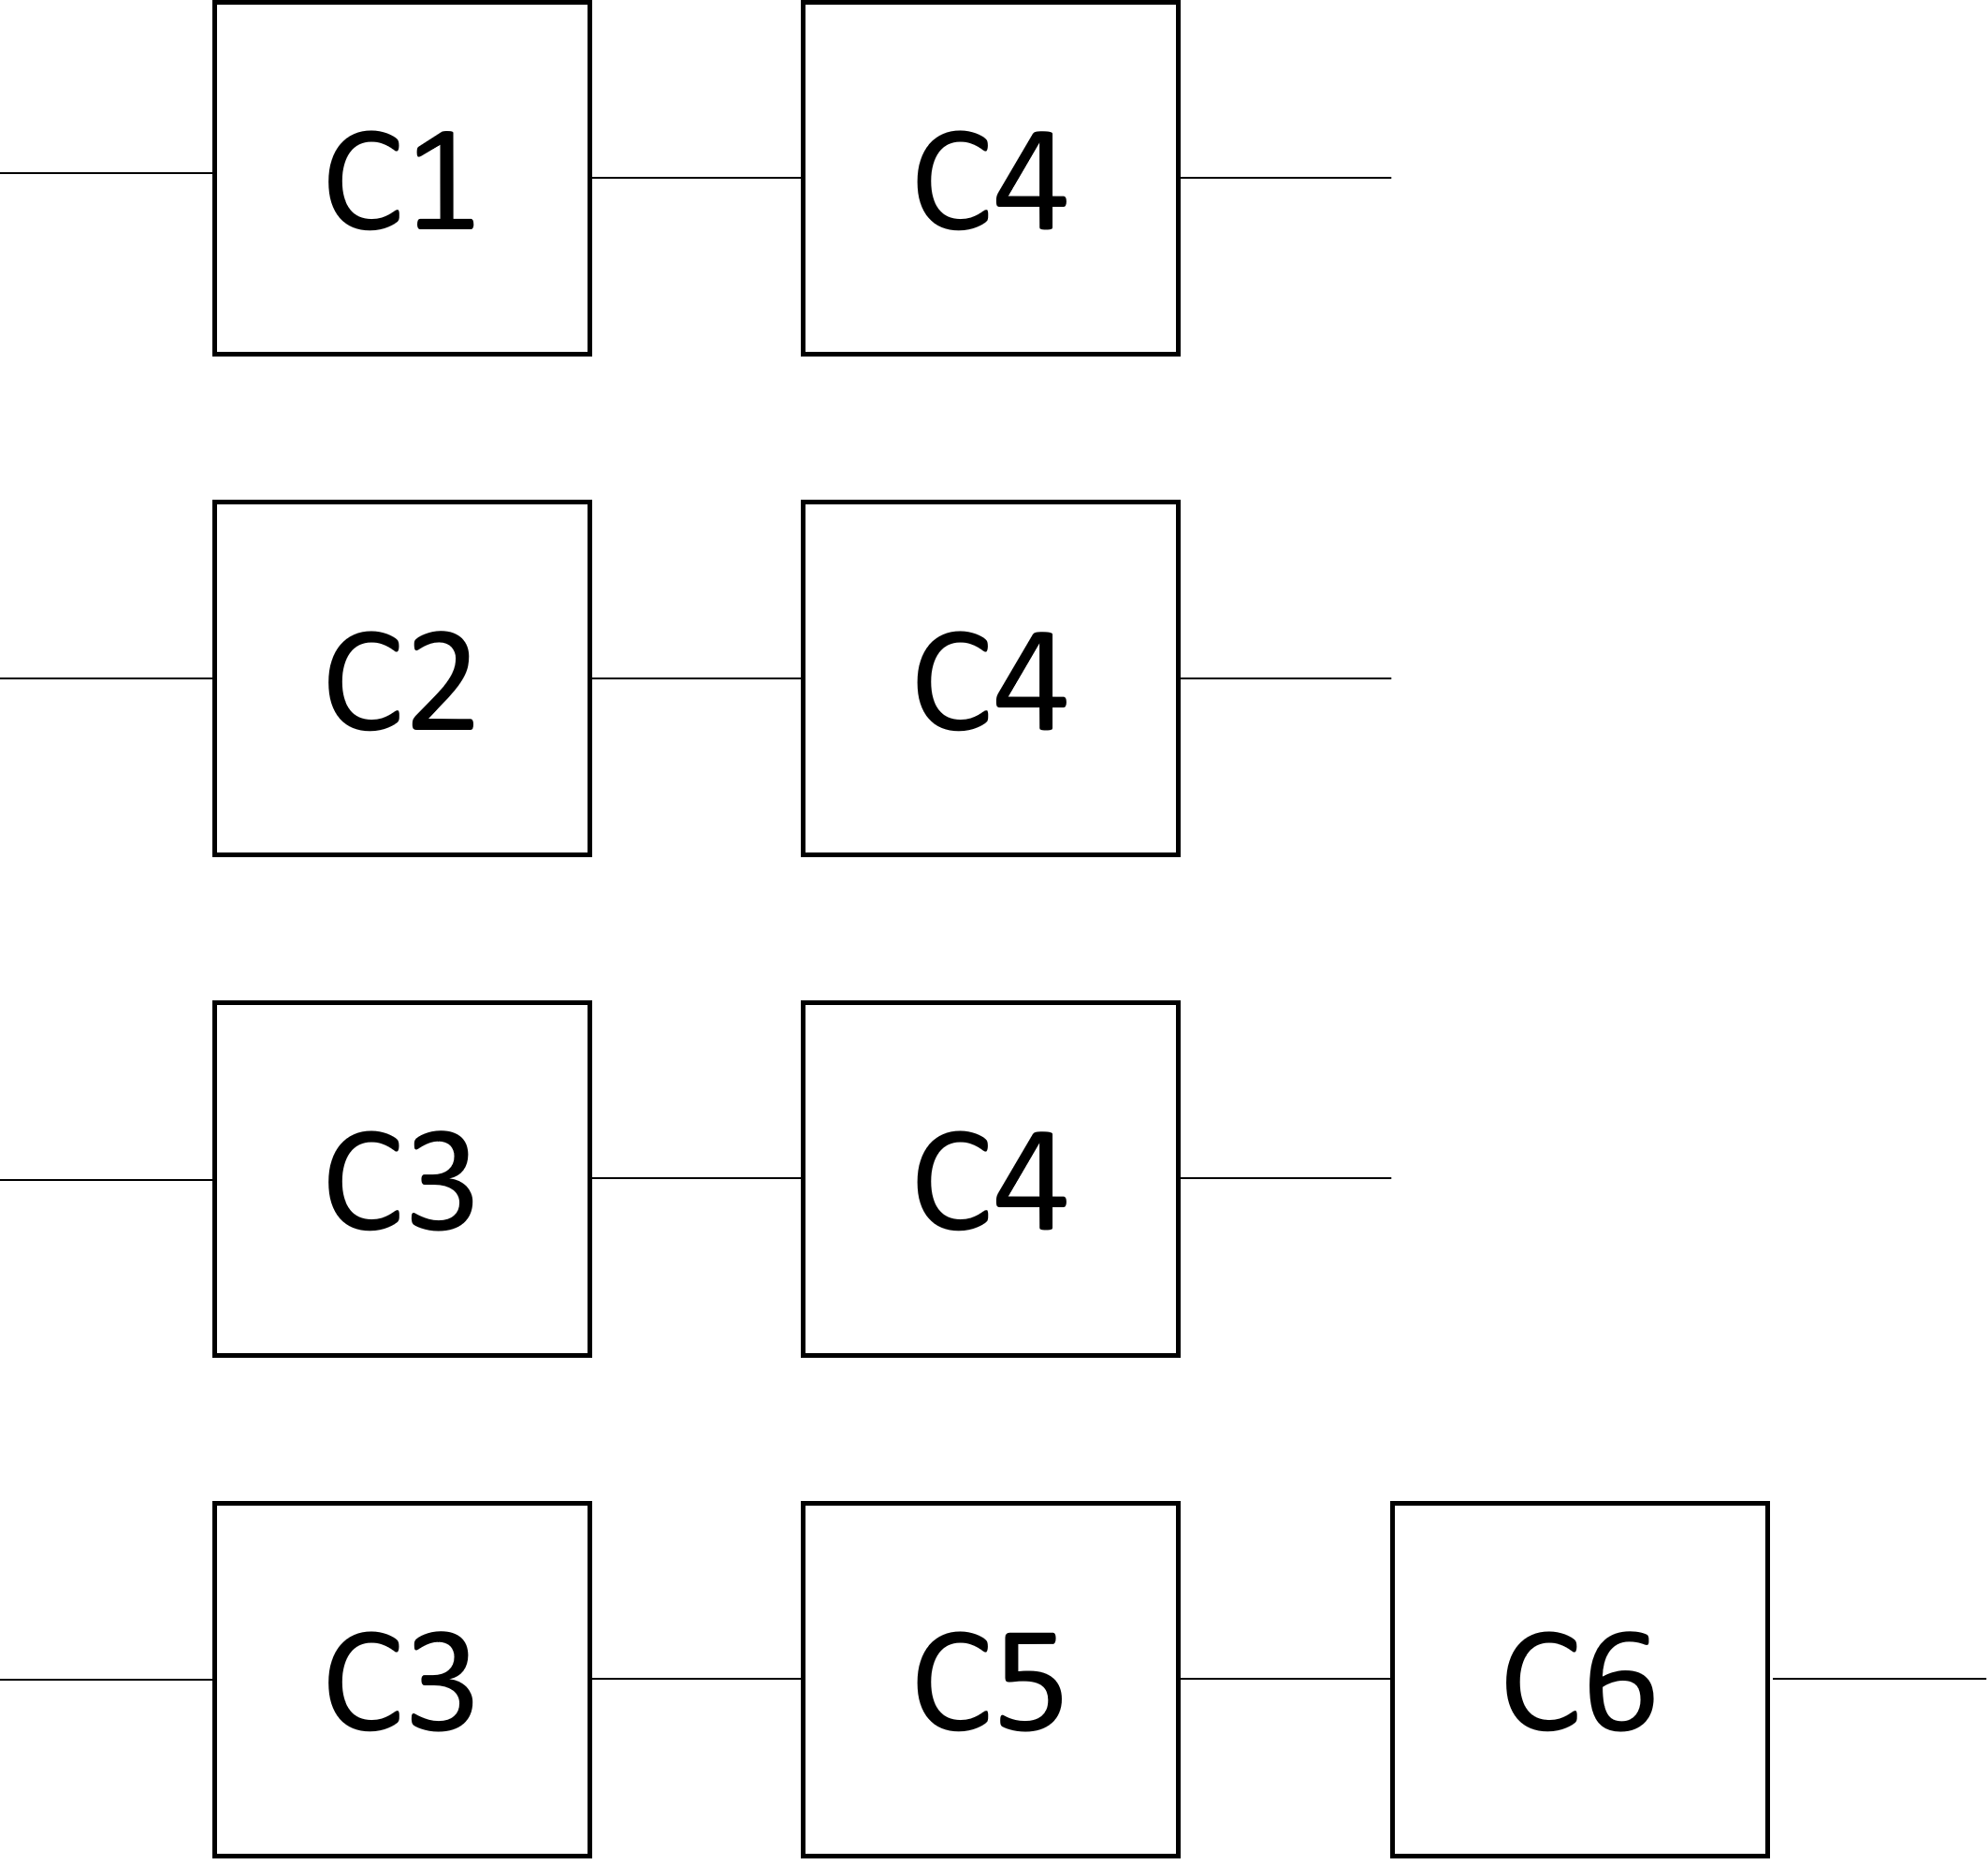
\includegraphics[width=0.5\textwidth]{img/ch5/upper_bound.png}
    \caption{Paths per l'upperbound}
    \label{fig:ex5_traccia}
\end{figure}

\newpage
\subsection{Conditioning}
Si è proceduto con l'analizzare il sistema quando il componente $C_3$ non funziona (assumendolo con un circuito aperto) e quando funziona (assumendolo con un cortocircuito) combinando i risultati mediante la probabilità totale. Quindi si ottiene:

\begin{equation*}
    R_{tot} = R_3 \cdot R_{C_3} + (1-R_3) \cdot R_{\overline{C}_3}
\end{equation*}

dove con $R_{C_3}$ si indica la \textit{reliability} del sistema laddove il componente $C_3$ funzioni; mentre con $R_{\overline{C}_3}$ si indica il sistema in cui $C_3$ non funzioni. Si risolvono i due diagrammi ottenuti \cref{fig:ex5_conditioning} in maniera indipendente.
\begin{figure}[H]
    \centering
    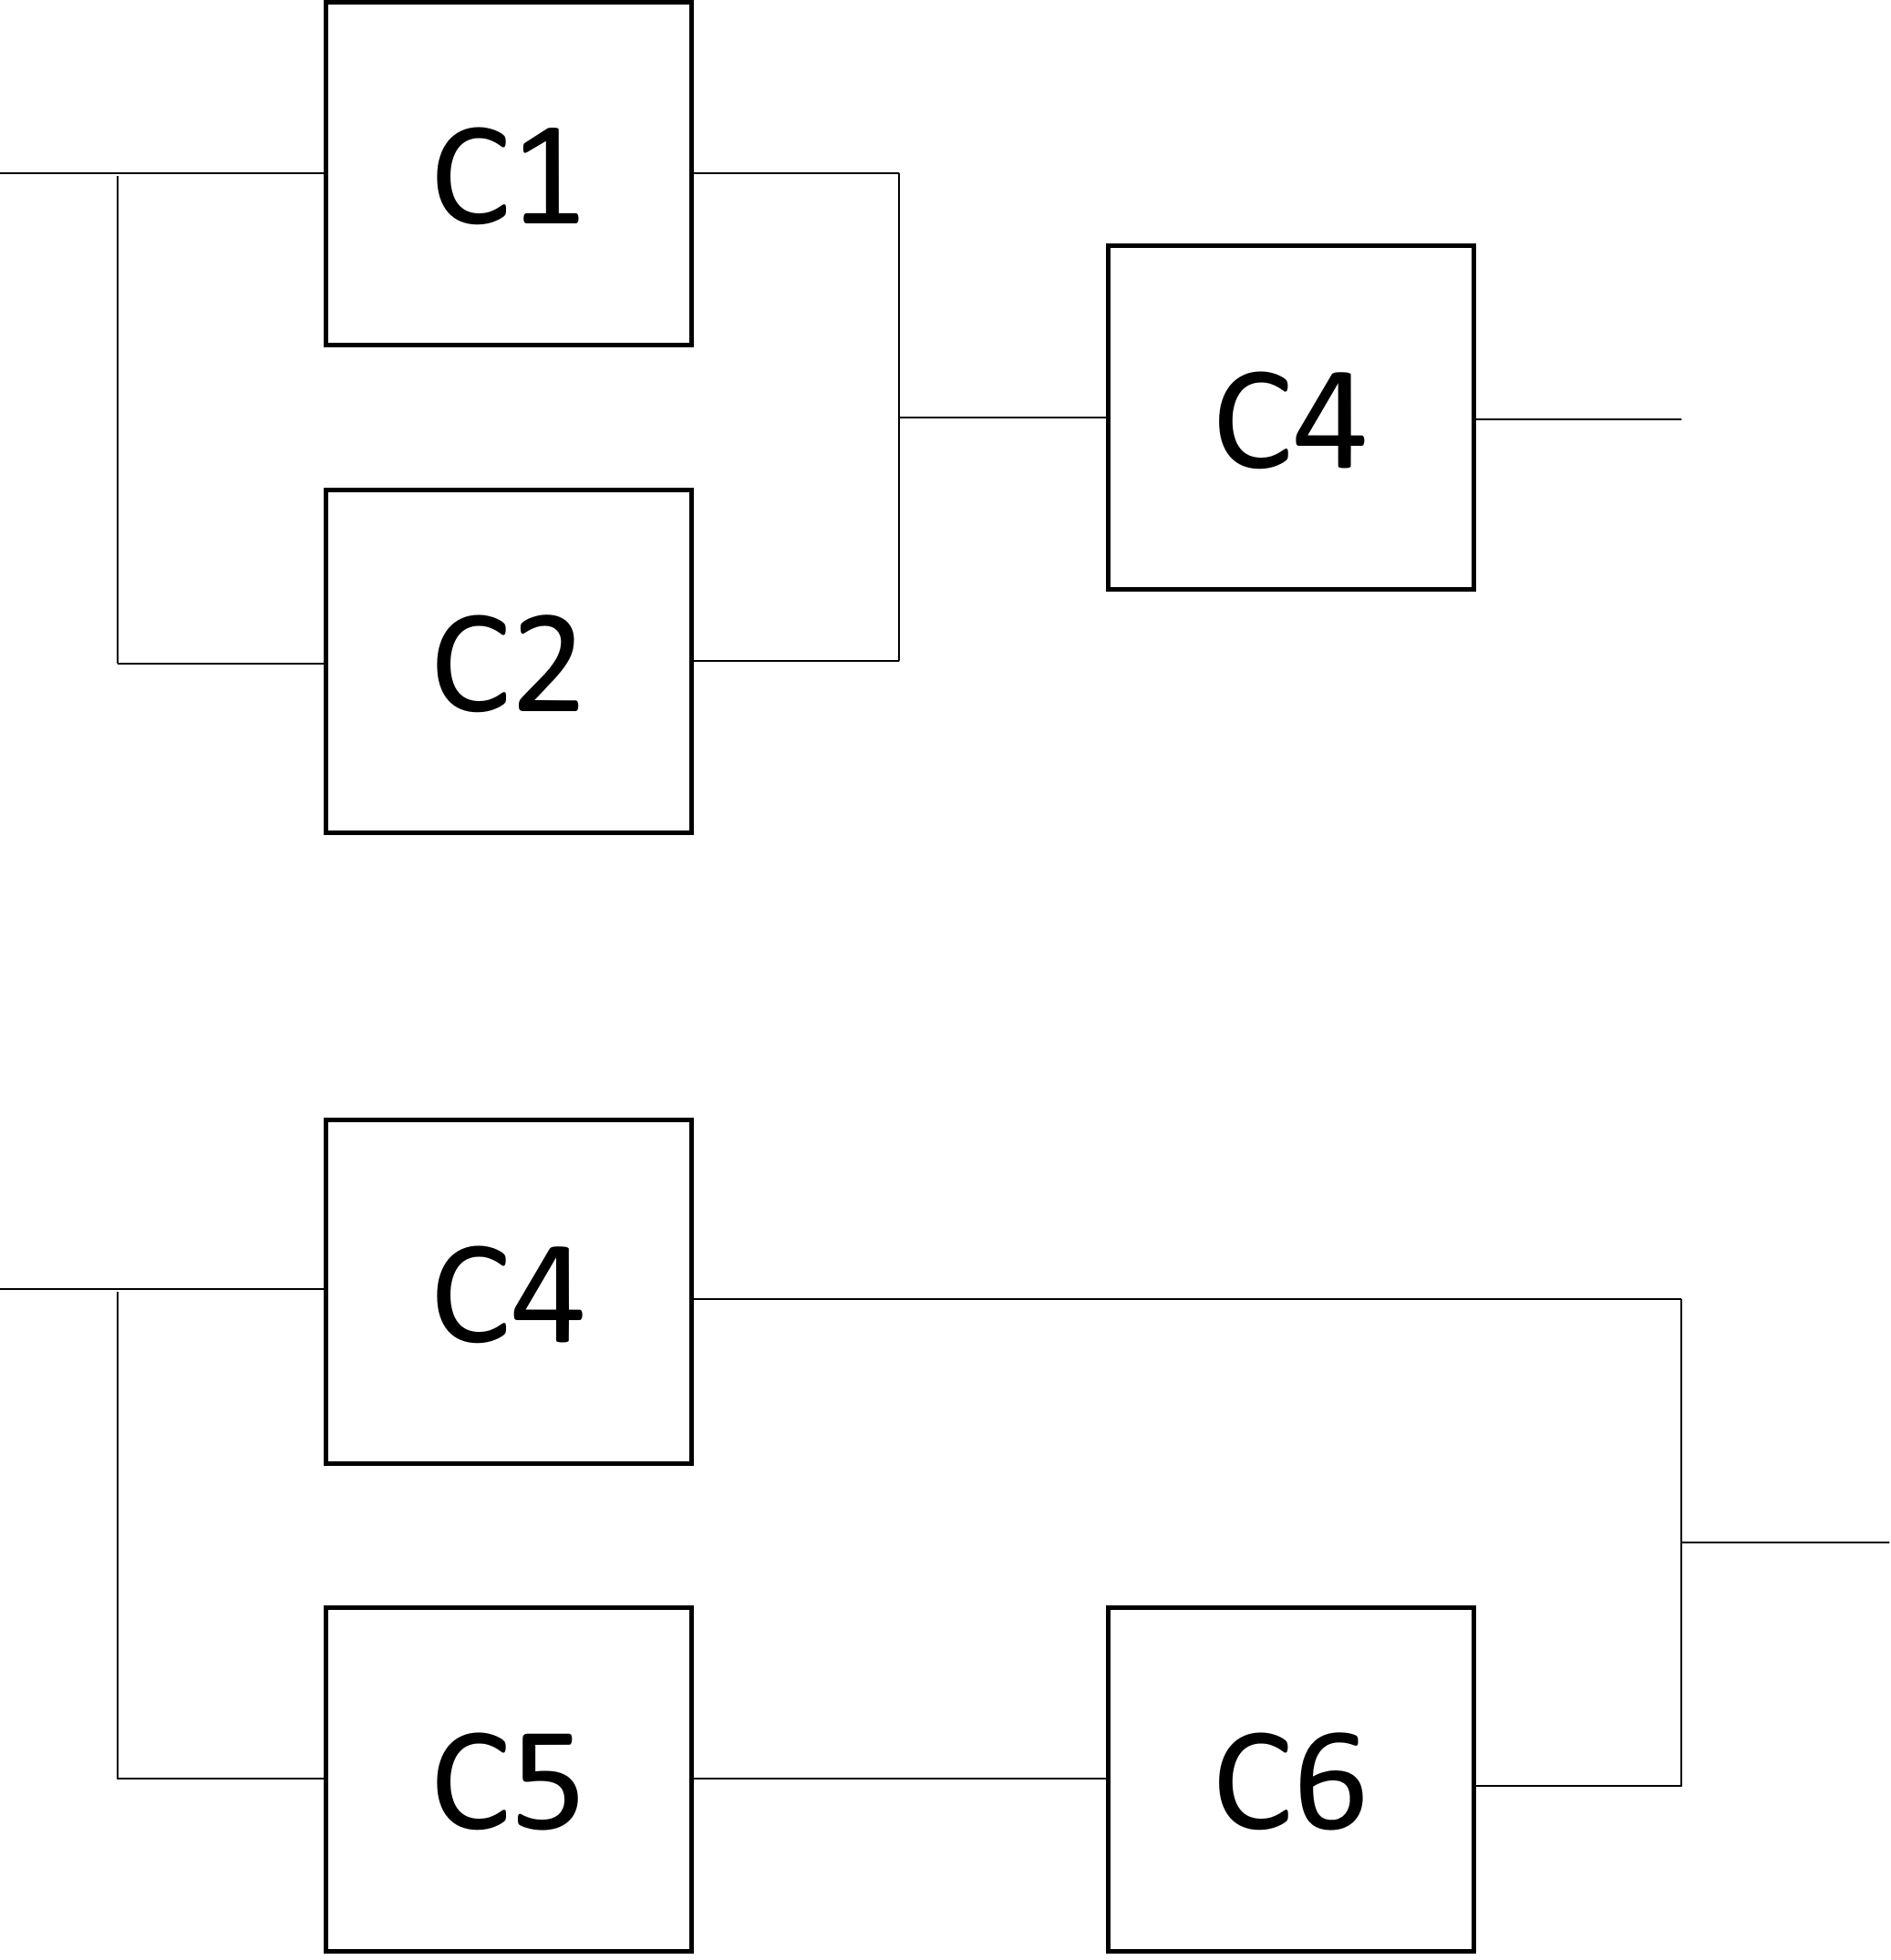
\includegraphics[width=0.5\textwidth]{img/ch5/conditioning.png}
    \caption{RBD con $C_3$ funzionante e non}
    \label{fig:ex5_conditioning}
\end{figure}

Nel caso in $C_3$ sia guasto, si ottiene:
\begin{equation*}
    R_{\overline{C}_3} = [1 - (1 - R_1) (1 - R_2)] R_4 = 2 e^{-2 \lambda t} - e^{-3 \lambda t}
\end{equation*}

Invece, quando $C_3$ funziona:

\begin{equation*}
    R_{C_3} = [1 - (1 - R_4) (1 - R_5R_6)] = -e^{-3 \lambda t} + e^{-2 \lambda t} + e^{-\lambda t}
\end{equation*}

Sostituendo i risultati ottenuti nell'espressione di $R_{tot}$:

\begin{align*}
    R_{tot} &= e^{-\lambda t} -e^{-3 \lambda t} + e^{-2 \lambda t} + e^{-\lambda t} + 2 e^{-2 \lambda t} - e^{-3 \lambda t} (1-e^{-\lambda t})\\
    &= -e^{-4 \lambda t} + e^{-3 \lambda t} + e^{-2 \lambda t} + e^{-4 \lambda t} - 3 e^{-3 \lambda t} + 2
    e^{-2 \lambda t} \\
    &= 3 e^{-2 \lambda t} - 2 e^{-3 \lambda t}
\end{align*}
\clearpage

\section{Exercise 2}
We want to compare two different schemes of increasing reliability of a system using redundancy. Suppose that the system needs s identical components in series for proper operation. Further suppose that we are given ($m x s$) components.  Given that the reliability of an individual component is R, derive the expressions for the reliabilities of two configurations. For $m = 2$ and $s = 4$, compare the two expressions as function of a mission time t.
Let MTTF of the component be $800$ hours.
Out of the two schemes shown in the figure below, which one will provide a higher reliability? Modify the scheme that has lower reliability in order to reach the same reliability of the other given the above MTTf ($800$ h).

\subsection{Calcolo e confronto della reliability dei due sistemi}
\begin{figure}[H]
    \centering
    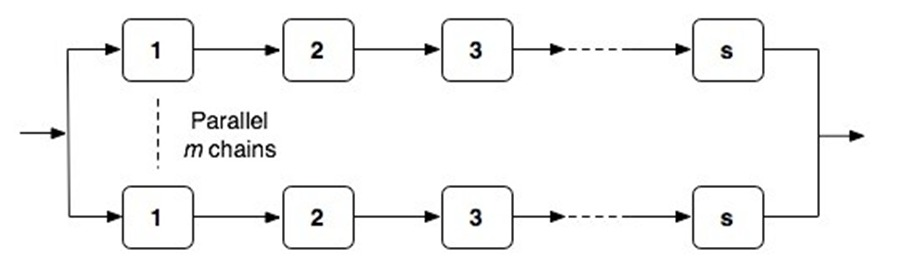
\includegraphics[width=0.8\textwidth]{img/ch5/exercise2.2.jpeg}
    \caption{Sistema 1}
    \label{fig:ex1_traccia}
\end{figure}

\begin{figure}[H]
    \centering
    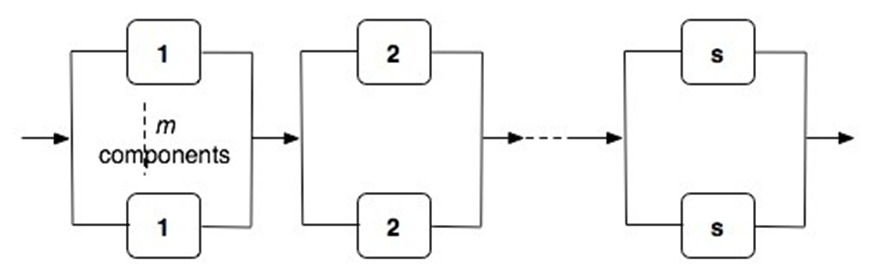
\includegraphics[width=0.8\textwidth]{img/ch5/exercise2.1.jpeg}
    \caption{Sistema 2}
    \label{fig:ex1_traccia}
\end{figure}

Per prima cosa sono state calcolate le reliability dei due sistemi, ottenute riducendoli in insiemi di serie e paralleli. In particolare, per il primo sistema ($m$ paralleli di $s$ serie) si è ottenuto il risultato in \cref{eq:m_sys1_res}; mentre per il secondo ($s$ serie di $m$ paralleli) si è ottenuto il risultato in \cref{eq:m_sys2_res}.

\begin{equation}
    R_{sys1} = 1 - (1 - R^s) ^ m
    \label{eq:m_sys1_res}
\end{equation}

\begin{equation}
    R_{sys2} = (1 - (1 - R)^m) ^ s
    \label{eq:m_sys2_res}
\end{equation}

Per $m=2$ e $s=4$, si ottiene:
\begin{equation*}
    R_{sys1} = 1 - (1 - R^4) ^ 2 = 1 - (1 - e{^{-4\lambda t}}) ^ 2
\end{equation*}
\begin{equation*}
     R_{sys2} = (1 - (1 - R)^m) ^ s = (1 - (1 - e{^{-\lambda t}})^2) ^ 4
\end{equation*}

Assegnato l'MTTF dei componenti uguale a 800 ore, quindi un  $\lambda=1/800$ sono stati tracciati i grafici relativi (mostrati in \cref{fig:ex5.2_comparazione}) alla reliability dei due sistemi al variare del tempo, da cui si evince che il sistema due sia più reliable del primo.

\begin{figure}[H]
    \centering
    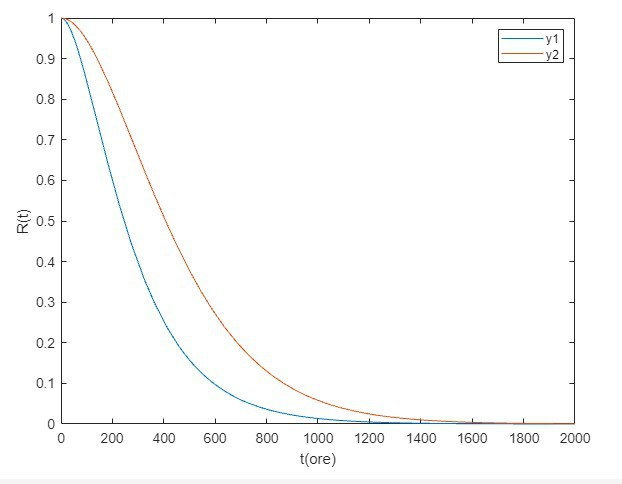
\includegraphics[width=0.8\textwidth]{img/ch5/comparison.png}
    \caption{Comparazione sistema 1 e sistema 2}
    \label{fig:ex5.2_comparazione}
\end{figure}


\subsection{Modifica del sistema 1}

Al fine di ottenere una reliability uguale a quella del sistema 2, si è fissato il tempo di missione per entrambi i sistemi a $800$ ore, facendo poi variare $m$ e ottenendo \cref{eq:ex5.2.3_soluzione}.

\begin{equation}
     0.1299 = 1 - (1-e^{-4\lambda t})^m; 
     \label{eq:ex5.2.3_soluzione}
\end{equation}

che ha come soluzione $ m \approx 7.53$, che approssimato per eccesso risulta essere $m=8$.

\begin{figure}[H]
    \centering
    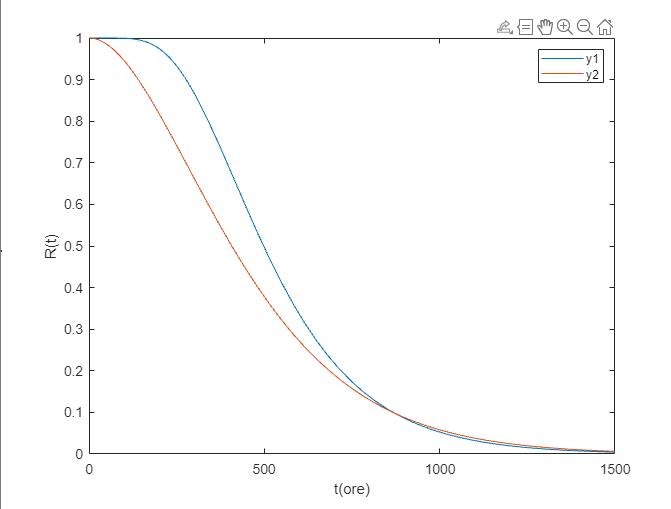
\includegraphics[width=0.8\textwidth]{img/ch5/s1_modified.png}
    \caption{Confronto \textit{reliability} tra $S_1$ modificato ($m=8$) $S_2$}
    \label{fig:ex5.2_comparazione}
\end{figure}

\clearpage
\section{Exercise 3}
The architecture of a network of computers in a banking system is shown below. The architecture is called a skip-ring network and is designed to allow processors to communicate even after node failures have occurred. For example, if node $1$ fails, node $8$ can bypass the failed node by routing data over the alternative link connecting nodes $8$ and $2$. Assuming the links are perfect and the nodes each have a reliability of $R_m$, derive and expression for the reliability of the network. If $R_m$ obeys the exponential failure law and the failure rate of each node is $0.005$ failures per hour, determine the reliability of the system at the end of a $48$-hour period.

\begin{figure}[H]
    \centering
    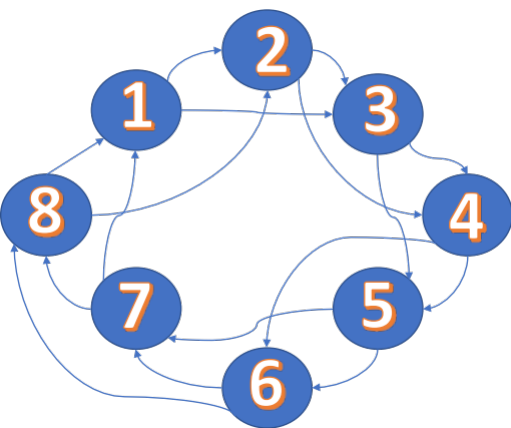
\includegraphics[width=0.5\textwidth]{img/ch5/3_traccia.png}
    \caption{Exercise 3}
    \label{fig:skip_ring}
\end{figure}

Partendo dalla topologia mostrata in \cref{fig:skip_ring} è stato ricavato il  fault tree in \cref{fig:fta_esercizio3}, che, come è possibile notare, presenta diversi eventi ripetuti.

\begin{figure}[H]
    \centering
    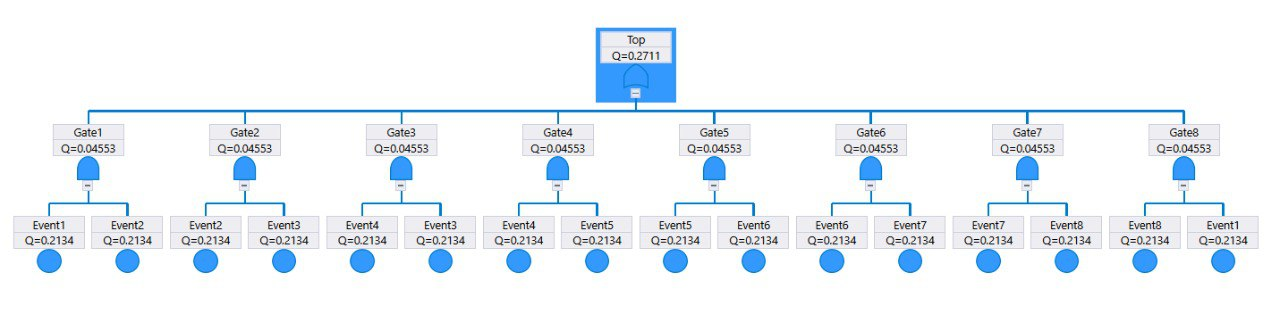
\includegraphics[width=\linewidth]{img/ch5/fta_esercizio3.png}
    \caption{Fault tree ricavato dalla \textit{skip ring network}}
    \label{fig:fta_esercizio3}
\end{figure}

A causa degli eventi ripetuti non è stato possibile convertire il fault tree in un RBD per calcolare la reliability.

È stato quindi utilizzato il metodo BDD, che converte i fault tree in Binary Decision Diagrams. Questi rappresentano l'equazione booleana che descrive il top event. Le probabilità possono quindi essere calcolate direttamente col BDD. 

Per farlo ci si è avvalsi del software \textit{TopEventFTA}, dove dopo aver costruito il Fault Tree, aver inserito le reliability dei componenti e fissando il tempo di missione a $48$ ore, la reliability del sistema risulta essere $0.728882$ .


\clearpage
\section{Exercise 4}
Compare the reliability of the following schemes, assuming an exponential failure occurrence with following values:
\begin{itemize}
    \item $MTTF_a=500$;
    \item $MTTF_b=9000$;
    \item $MTTF_c=1000$;
\end{itemize}

\begin{figure}[H]
    \centering
    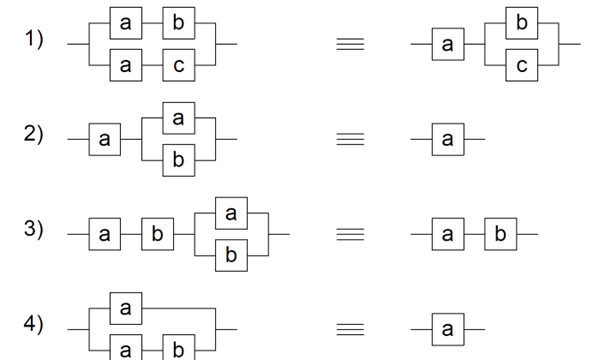
\includegraphics[width=0.8\textwidth]{img/ch5/exercise_4.png}
    \caption{Exercise 4}
    \label{}
\end{figure}

\paragraph{Punto 1}

Sono state calcolate le reliability per i due schemi, $y_1$ e  $y_2$, e ne è stato fatto il confronto in \cref{fig:4.1_cmp}.

\begin{itemize}
    \item $y_1  = 1-(1 - R_aR_b) \cdot (1 - R_aR_c)$
    \item $y_2  = R_a\cdot(1 - (1-R_b)) \cdot (1 - R_c)$
\end{itemize}

\begin{figure}[H]
    \centering
    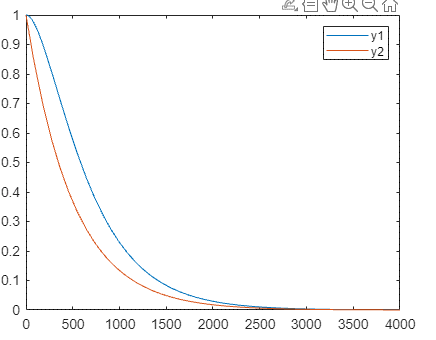
\includegraphics[width=0.8\textwidth]{img/ch5/4.1.png}
    \caption{Comparazione reliability punto 1}
    \label{fig:4.1_cmp}
\end{figure}

Si osserva che nello schema a destra il componente $a$ si comporta da \textit{single point of failure} per il sistema. In quello a sinistra, essendoci un parallelo e due copie di $a$ il sistema risulta più \textit{reliable}.

\paragraph{Punto 2}

Sono state calcolate le reliability per i due schemi, $y_1$ e  $y_2$, e ne è stato fatto il confronto in \cref{fig:4.2_cmp}.

\begin{itemize}
    \item $y_1  = R_a\cdot(1 - (1-R_b) \cdot (1 - R_a))$
    \item $y_2  = R_a$
\end{itemize}

\begin{figure}[H]
    \centering
    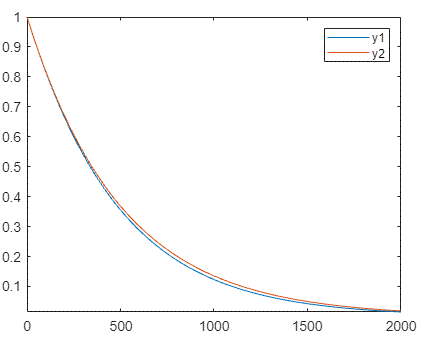
\includegraphics[width=0.8\textwidth]{img/ch5/4.2.png}
    \caption{Comparazione reliability punto 2}
    \label{fig:4.2_cmp}
\end{figure}
Si osserva che, prevedibilmente, il sistema 2 ha una reliability più alta. Il sistema a sinistra è infatti una serie di componenti di cui A fa parte, e avrà per forza una reliability generica del tipo $Ra\cdot R_i$ (dove $R_i$ corrisponde alla reliability del resto della serie) che essendo un prodotto di probabilità sarà sicuramente $\leq Ra$.


\paragraph{Punto 3}

Sono state calcolate le reliability per i due schemi, $y_1$ e  $y_2$, e ne è stato fatto il confronto in \cref{fig:4.3_cmp}.

\begin{itemize}
    \item $y_1  = R_aR_b\cdot(1 - (1-R_b) \cdot (1 - R_a))$
    \item $y_2  = R_aR_b$
\end{itemize}

\begin{figure}[H]
    \centering
    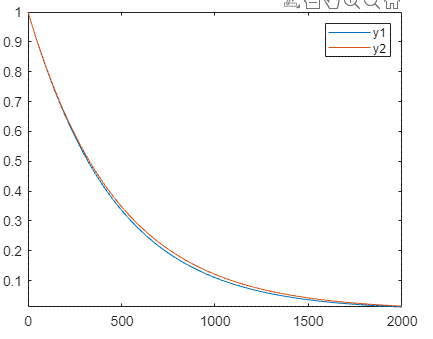
\includegraphics[width=0.8\textwidth]{img/ch5/4.3.png}
    \caption{Comparazione reliability punto 3}
    \label{fig:4.3_cmp}
\end{figure}
Si osserva che, prevedibilmente, il sistema 2 ha una reliability più alta. Il sistema a sinistra è infatti una serie di componenti di cui A-B fa parte, e avrà per forza una reliability generica del tipo $Rab\cdot R_i$ (dove Ri corrisponde alla reliability del resto della serie) che essendo un prodotto di probabilità sarà sicuramente $\leq Rab$.


\paragraph{Punto 4}

Sono state calcolate le reliability per i due schemi, $y_1$ e  $y_2$, e ne è stato fatto il confronto in \cref{fig:4.4_cmp}.

\begin{itemize}
    \item $y_1 = 1-((1 - R_a) \cdot (1 - R_bR_a))$
    \item $y_2 = R_a$
\end{itemize}

\begin{figure}[H]
    \centering
    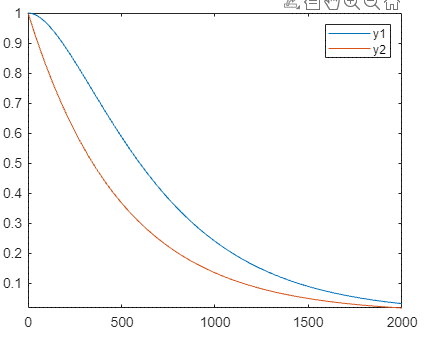
\includegraphics[width=0.8\textwidth]{img/ch5/4.4.png}
    \caption{Comparazione reliability punto 4}
    \label{fig:4.4_cmp}
\end{figure}

Il sistema a sinistra risulta più affidabile di quello di destra. Si può osservare come, al netto del componente B, il sistema a sinistra risulta un parallelo di componenti A e che la presenza di B peggiora solo la reliability. In questo caso però, dato che l'MTTF di B è di un ordine di grandezza superiore a quello di A il suo impatto è marginale.

\newpage
\section{Exercise 5}
The system shown in the figure below is a processing system for a helicopter. The system has dual-redundant processors and dual-redundant interface units. Two buses are used in the system, and each bus is also dual-redundant. The interesting part of the system is the navigation equipment. The aircraft can be completely navigated using the Inertial Navigation System (INS). If the INS fails, the aircraft can be navigated using the combination of the Doppler and the altitude heading and reference system (AHRS). The system contains three AHRS units, of which only one is needed. This is an example of functional redundancy where the data from the AHRS and the Doppler can be used to replace the INS, if the INS fails. Because of the other sensors and instrumentation, both buses are required for the system to function properly regardless of which navigation mode is being employed. 

\begin{figure}[H]
    \centering
    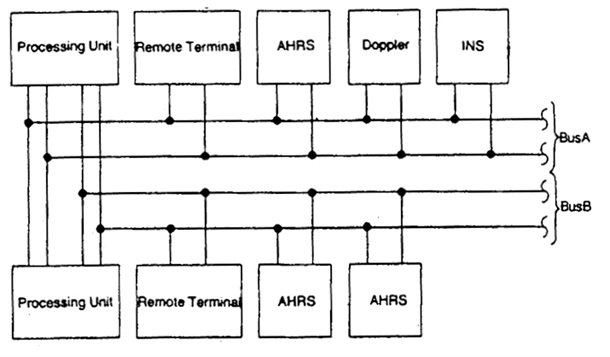
\includegraphics[width=0.8\textwidth]{img/ch5/exercise_5.png}
    \caption{Exercise 5}
\end{figure}

\begin{itemize}
    \item a) Draw the reliability block diagram of the system.
    \item b) Draw the Fault Tree of the system and analyze the minimal cutsets.
    \item c) Calculate the reliability for a one-hour flight using the MTTF figures given in the table below. Assume that the exponential failure low applies and that the fault coverage is perfect.
    \item d) Repeat (c), but this time, incorporate a coverage factor for the fault detection and reconfiguration of the processing units. Using the same failure data, determine the approximate fault coverage value that is required to obtain a reliability (at the end of one hour) of 0.99999.

\end{itemize}

\begin{figure}[H]
    \centering
    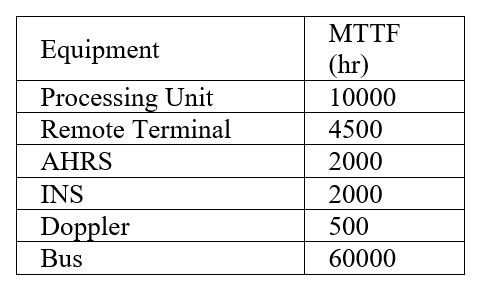
\includegraphics[width=0.5\textwidth]{img/ch5/tabella.png}
\end{figure}

\paragraph{Punto A}
Un \textit{RBD} è un diagramma che mostra il sistema dividendolo in più moduli, ognuno con una probabilità di funzionare $p$ o una reliability $R$, con lo scopo di calcolare la reliability generale.
Ogni modulo o componente è rappresentato solo una volta nel grafico, e i fallimenti sono indipendenti tra loro. Una volta fallito,si ritiene che il modulo darà sempre risultati sbagliati.

Il sistema inoltre verrà definito non funzionante quando non contiene un minimo set di moduli funzionanti, e una volta che entra nello stato di fallimento non potrà tornare a funzionare tramite altri fallimenti.

Per disegnare il \textit{reliability block diagram} sono state analizzate le relazioni tra i componenti, in modo da inserire in parallelo quelli ridondanti,e in serie quelli per cui un fallimento compromette il funzionamento del sistema.

In particolare, è possibile ridurre il sistema in più sottosistemi in serie, all'interno dei quali abbiamo diversi componenti in parallelo:
\begin{itemize}
    \item CPU: composto dal parallelo di CPU1 e CPU2
    \item BUS A: composto dal parallelo di BusA1 e BusA2
    \item BUS B: composto dal parallelo di BusB1 e BusB1
    \item Sistema di navigazione: composto dal parallelo tra INS e una serie di Doppler e tre ASHRS3 in parallelo
    \item Terminale remoto: composto dal parallelo di Remote Terminal 1 e Remote Terminal 2
\end{itemize}

\begin{figure}[H]
    \centering
    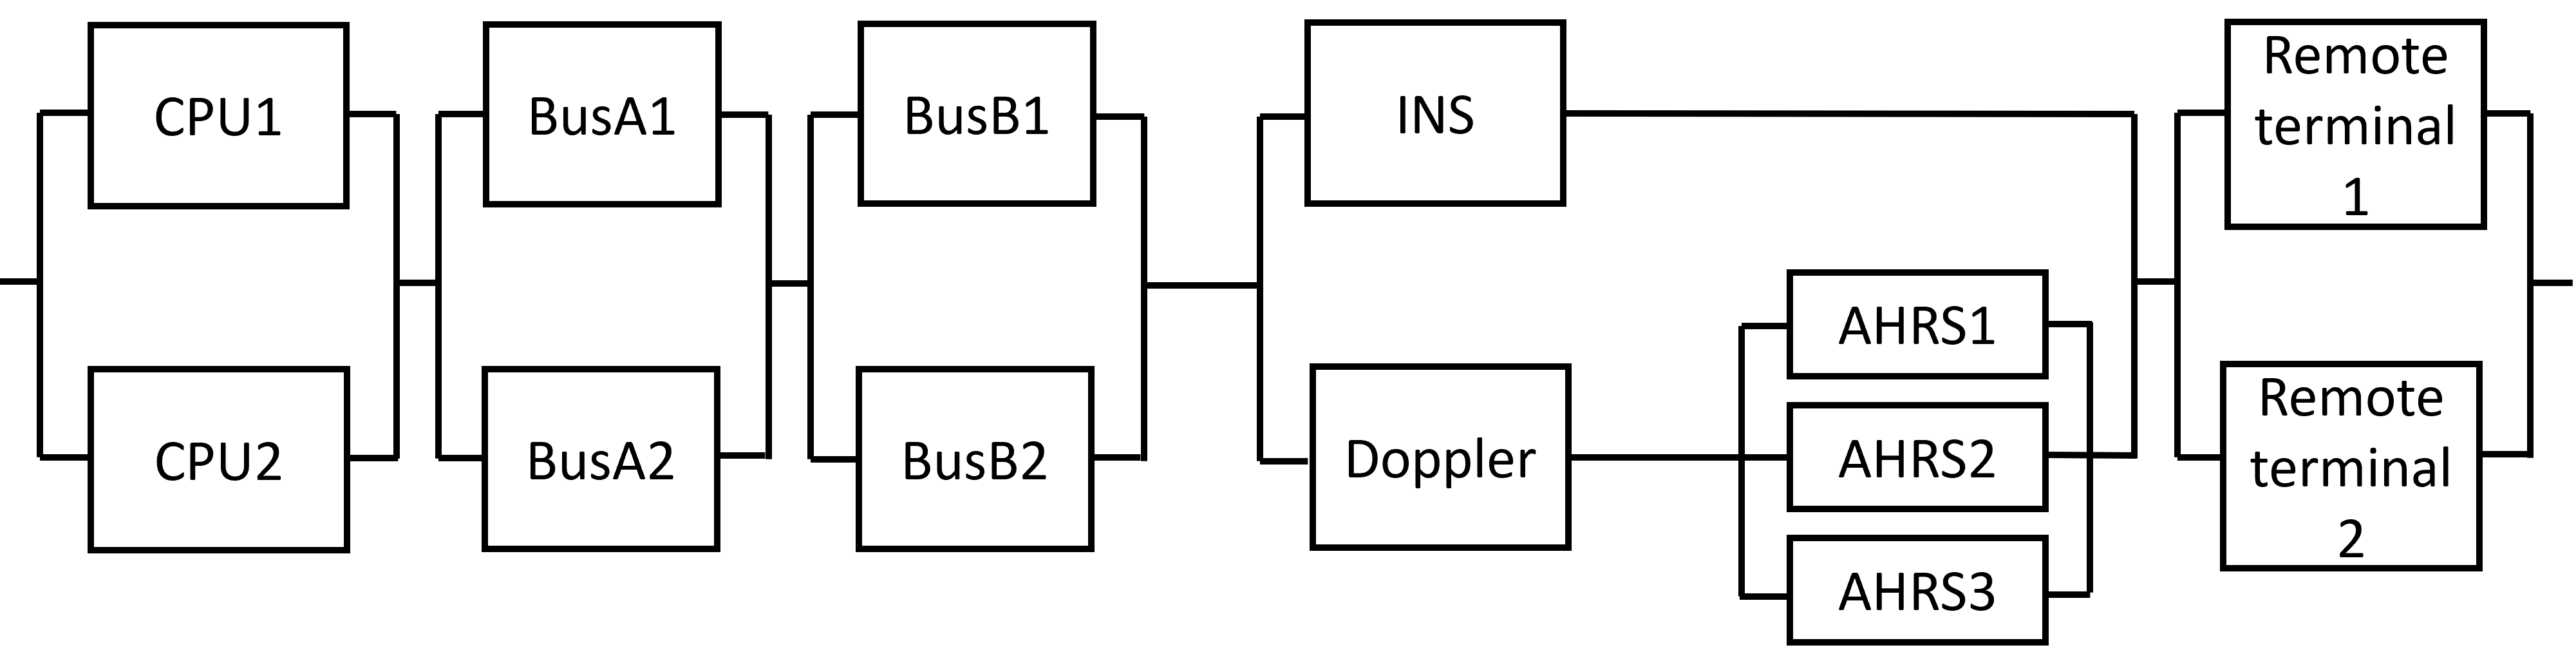
\includegraphics[width=0.8\textwidth]{img/ch5/helicopter_rbd.png}
    \caption{RBD del sistema}
    \label{fig:4.5_rbd}
\end{figure}

\paragraph{Punto B}
Un \textit{Fault Tree} è una rappresentazione grafica delle combinazioni di eventi che possono portare a un fallimento del sistema.
Le cause al più basso livello sono chiamati eventi base.
Ogni componente è rappresentato come un nodo, interconnesso con gli altri tramite porte logiche, e il fallimento di uno di questi porta l'input della porta a cui è collegato a diventare alto.

Per ottenere il \textit{fault tree} è possibile partire dal \textit{reliability block diagram} e trasformare le serie di componenti in una OR e i paralleli in \textit{AND}.

\begin{figure}[H]
    \centering
    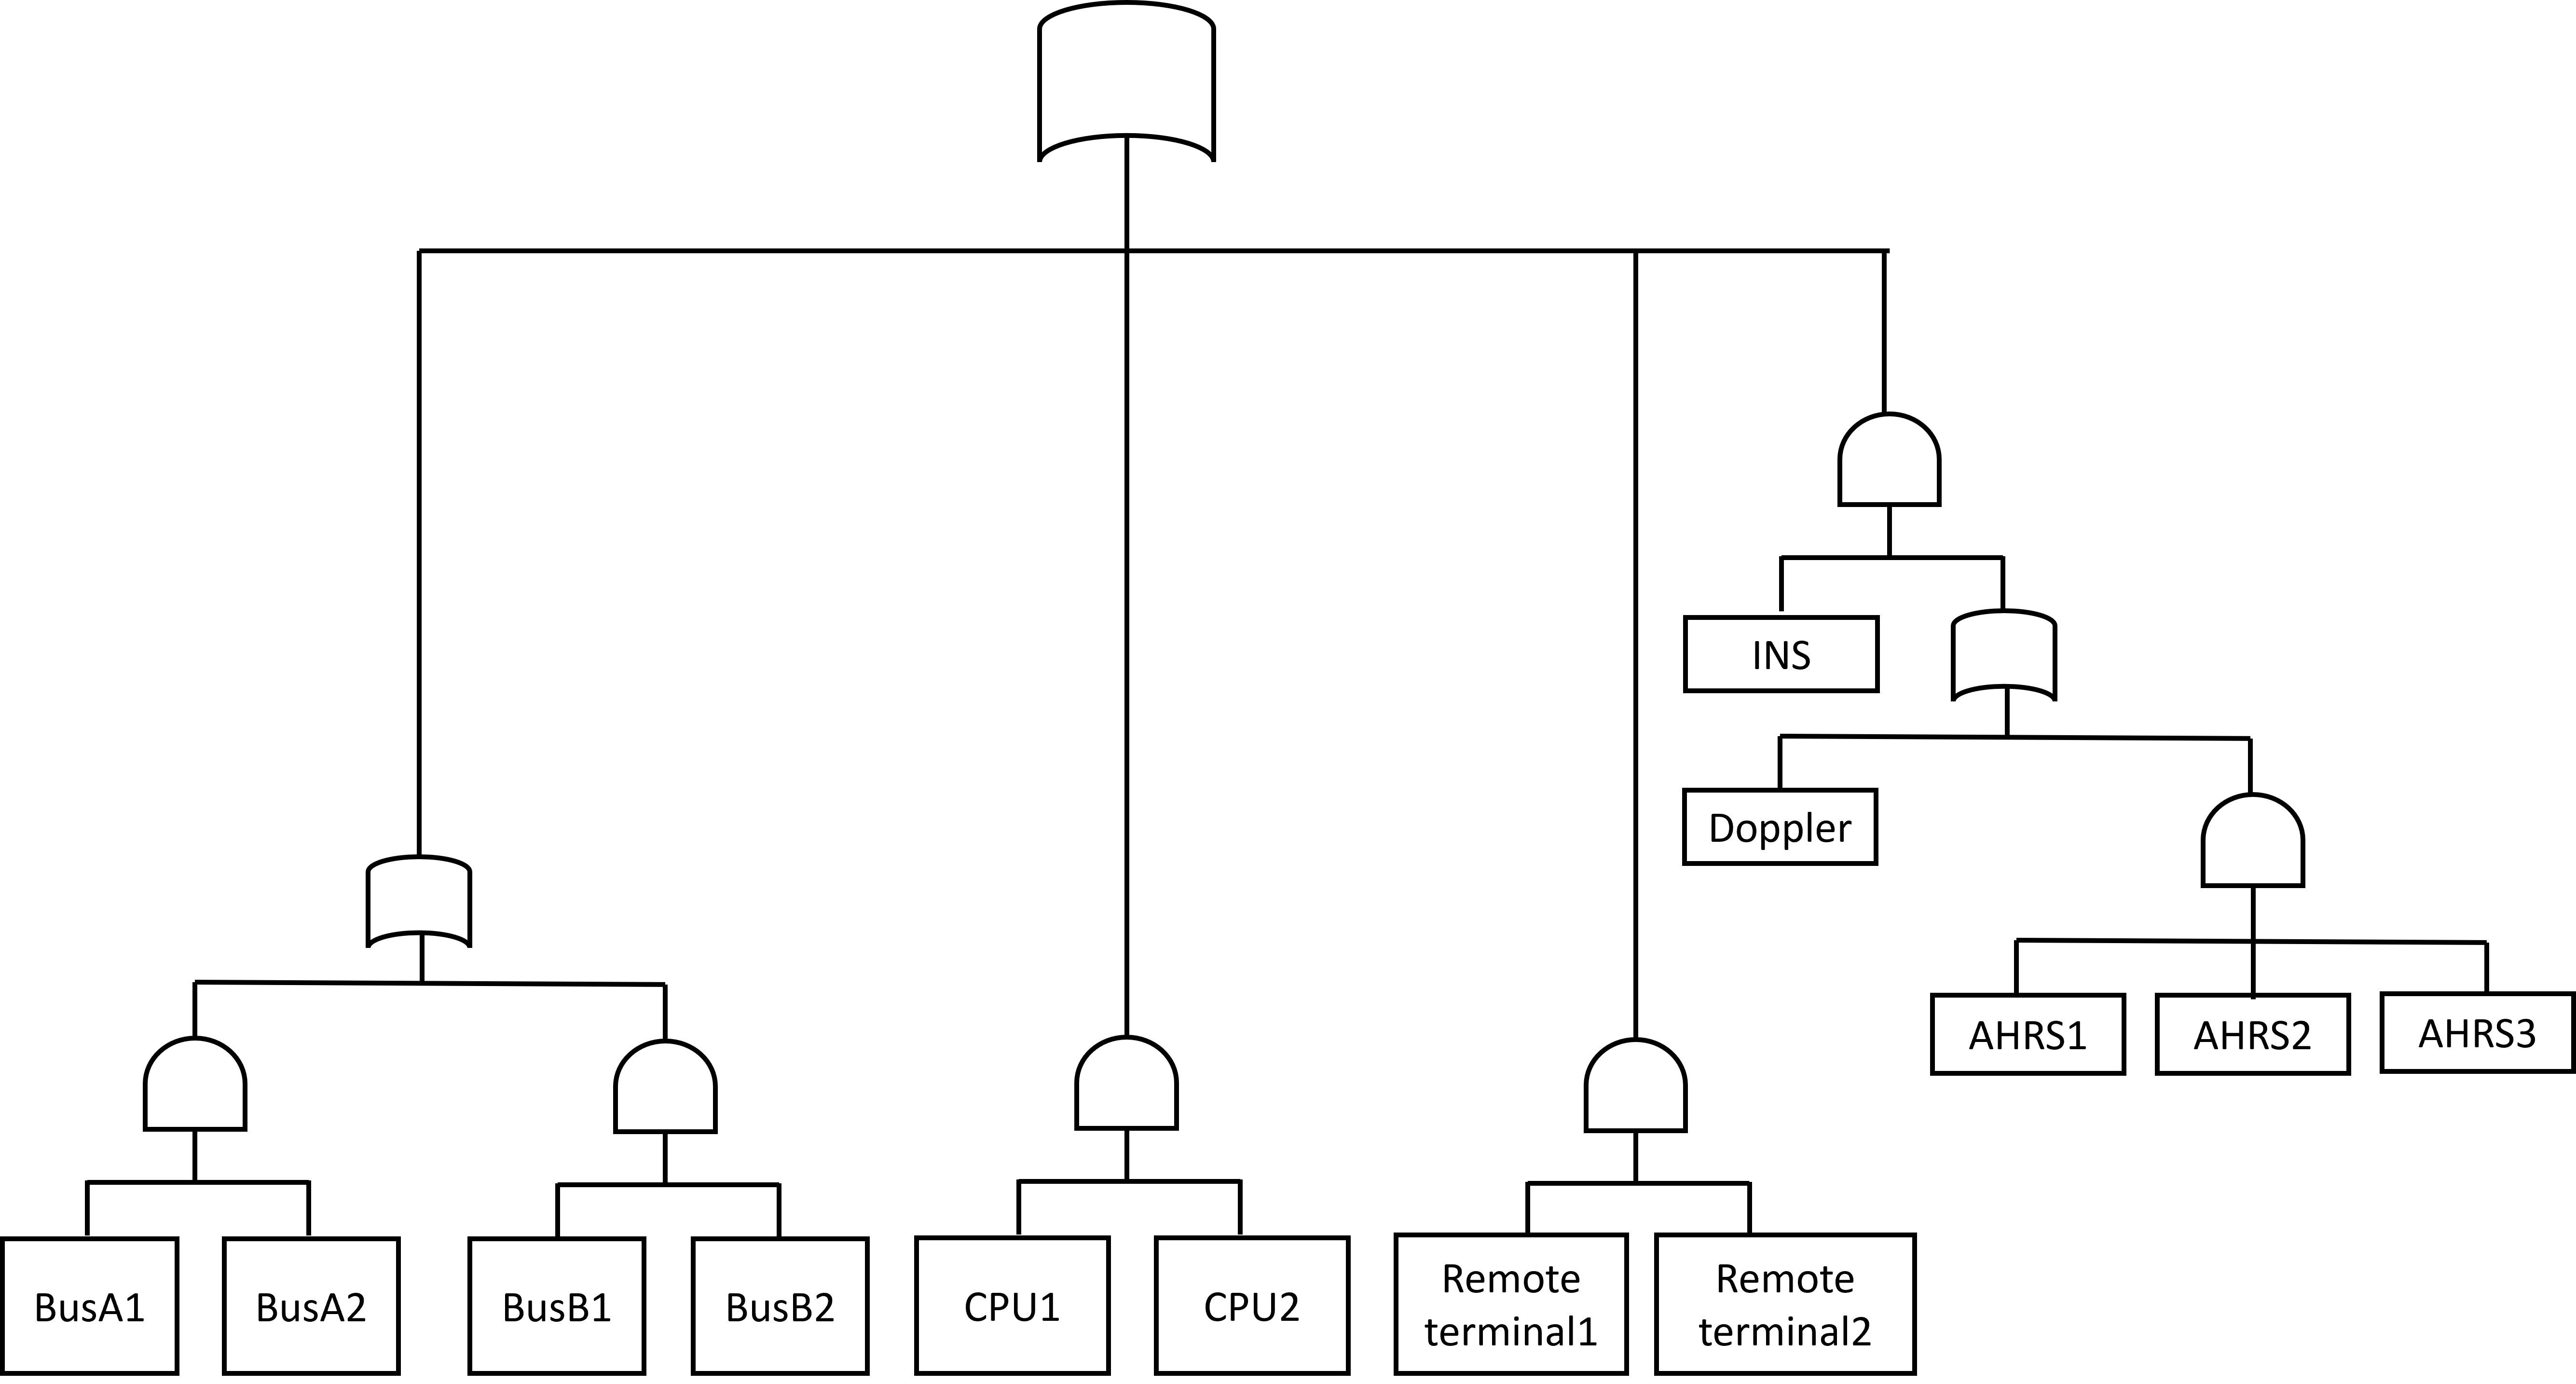
\includegraphics[width=0.8\textwidth]{img/ch5/fault_tree_helicopter.png}
    \caption{Fault tree del sistema}
    \label{fig:4.5}
\end{figure}

Il \textit{Minimal Cut Set} è definito come il più piccolo insieme di eventi base che, in congiunzione, possono causare il top level event, cioè il fallimento del sistema.
Di seguito sono mostrati i set trovati:
\begin{itemize}
    \item BUSA1 \land BUSA2
    \item BUSB1 \land BUSB2
    \item CPU1 \land CPU2
    \item Remote Terminal 1 \land Remote Terminal 2
    \item INS \land Doppler
    \item INS \land AHRS1 \land AHRS2 \land AHRS1 3
\end{itemize}

\paragraph{Punto C}
Partendo dall'RBD in \cref{fig:4.5_rbd} è possibile applicare le relazioni fondamentali di serie e parallelo. In particolare, si arriva alla relazione mostrata di seguito.

\begin{align*}
    R_{tot}&=(1-(1-R_{ter})^2) \cdot (1-(1-R_{cpu})^2)\\
    &\cdot(1-(1-R_{bus})^2)^2\cdot(1-(1-R_{ins})\\
    &\cdot(1-R_{dop}\cdot(1-(1-R_{ahrs})^3)))
\end{align*}

Sostituendo i dati del problema, si ottiene $R_{tot} = 0.99999894132275$.

\paragraph{Punto D}

La failure detection non è una tecnica perfetta, quindi nel caso di sistemi ridondati può essere possibile che un fault non venga rilevato. Questo possibile punto di fallimento del sistema viene modellato con l'introduzione di un componente $c$ in serie al sistema totale. Quindi, ad esempio, per un solo elemento ridondato, la reliability del parallelo è:
\begin{equation*}
    R = R_1 + c ( 1 - R_1)R_2
\end{equation*}
Nell'esercizio è richiesto di stimare il fattore $c$, immaginando di avere un fault detector non ideale solo per i componenti \textit{CPU1} e \textit{CPU2}, mantenendo una reliability pari a $0.99999$. Quindi, si è proceduto con riscrivere la relazione di \textit{reliability} utilizzando come incognita $c$.

\begin{align*}
    R_{tot}&=(1-(1-R_{ter})^2) \cdot (R_{cpu}+ c \cdot (1-R_{cpu}) \cdot R_{cpu}))\\
    \label{eq:rel_fault_coverage}
    &\cdot(1-(1-R_{bus})^2)^2\cdot(1-(1-R_{ins})\\
    &\cdot(1-R_{dop}\cdot(1-(1-R_{ahrs})^3)))
\end{align*}

Risolvendo l'equazione per $c$, si ottiene $c = 0.9106$.

\chapter{FFDA}

\section{Traccia}
Conduct the analysis for MercuryErrorLog.txt and BGLError-Log.txt:
\begin{itemize}
    \item tuple count plot + selected CWIN;
    \item grouping entries with selected CWIN;
    \item empirical reliabilities distributions;
    \item fit the empirical reliabilility (try all the models- exponential, hy-
perexponential, weibull);
\end{itemize}

Answer the following :
\begin{itemize}
    \item Can the same coalesce windows be used across different
nodes (Mercury, BG/L) and error categories (Mercury) ?
    \item  What about the relationship between the system reliability
and nodes reliability?
    \item there exist dependability-bottlenecks (i.e., topcontributors to the total number of failures)?
    \item Do similar functional nodes (e.g., two Mercury tg-cX computing nodes or BG/L I/O nodes Ri:Mx:Nz) exhibit similar reliability parameters?
    \item there exist a relationship between the error types and the node (Mercury)?
\end{itemize}

\newpage
\section{Mercury}
Il super-calcolatore \textit{Mercury} consiste in una serie di nodi organizzati in un'architettura a tre livelli a cui si aggiunge un nodo di management (\cref{fig:mercury_arch}).

\begin{figure}[H]
    \centering
    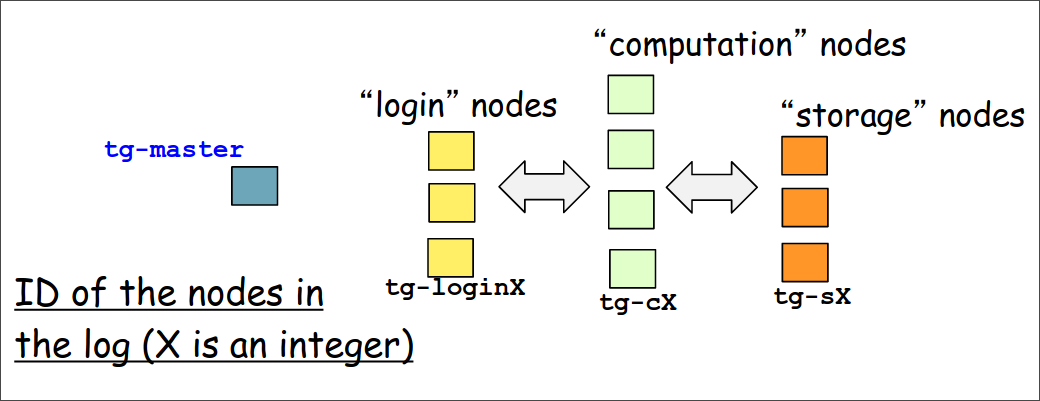
\includegraphics[width=0.8\textwidth]{img/ch6/mercury_architecture.png}
    \caption{Architettura multi-livello del supercal-calcolatore Mercury}
    \label{fig:mercury_arch}
\end{figure}

Gli altri nodi sono:
\begin{itemize}
    \item Login;
    \item Computation;
    \item Storage;
\end{itemize}

Il file in ingresso MercuryErrorLog.txt contiene $80854$ entry ciascuna delle quali ha il formato \textit{timestamp - nodo - categoria - messaggio di errore}.


\subsection{Temporal coalescence }
Partendo dal file dei log si vuole diminuire il numero di entries raggruppando quelle che possono essere relative allo stesso fault. Per farlo è stata applicata la tecnica della coalescenza temporale in cui, una definita una finestra temporale $W$, si pongono all'interno della stessa tupla tutti gli eventi con differenza di timestamp minore di $W$ come scritto nella \cref{eq:coal_window}.

\begin{equation}
    X(t+1) - X(t) < W
    \label{eq:coal_window}
\end{equation}

La difficoltà principale nell'utilizzo di questa tecnica è il calcolo della \textit{window size}.
Nel caso sia troppo piccola porta a dei fenomeni di \textit{trucation} (\cref{fig:ex_truncation}), in cui eventi relativi allo stesso fault vengono messi in tuple diverse, e viceversa si possono verificare \textit{collisions} ( (\cref{fig:ex_collision}) con $W$ troppo grandi, in cui eventi relativi a fault diversi vengono raggruppati insieme.

\begin{figure}[H]
    \centering
    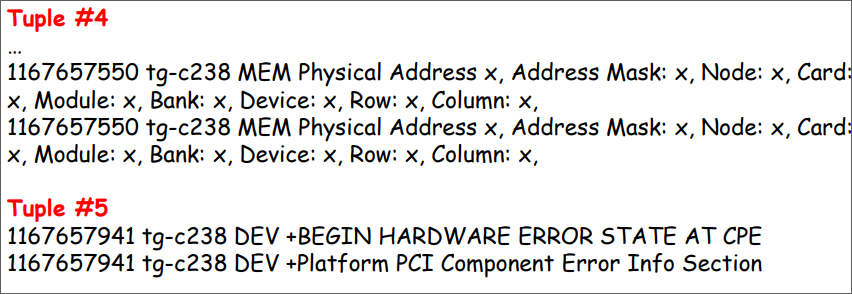
\includegraphics[width=0.8\textwidth]{img/ch6/ex_truncation.png}
    \caption{Esempio di truncation}
    \label{fig:ex_truncation}
\end{figure}

\begin{figure}[H]
    \centering
    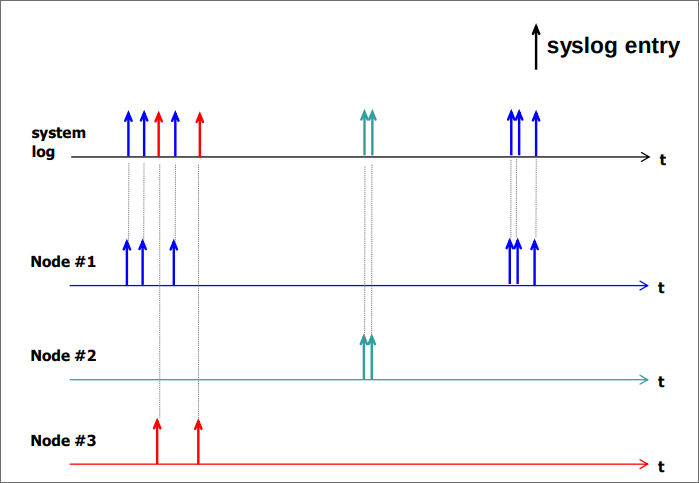
\includegraphics[width=0.8\textwidth]{img/ch6/ex_collision.png}
    \caption{Esempio di collisione}
    \label{fig:ex_collision}
\end{figure}

Per trovare un valore ottimale di W è stata effettuata una \textit{Sensitivity Analysis}, calcolando il numero di tuple generate a seconda di multipli valori della \textit{window size}.

Il risultato ottenuto è visibile in figura \cref{fig:mercury_cwin}.

\begin{figure}[H]
    \centering
    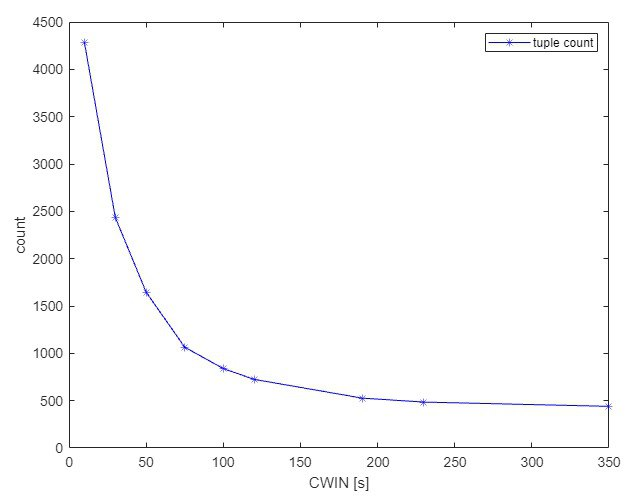
\includegraphics[width=0.8\textwidth]{img/ch6/merc_cwin.png}
    \caption{}
    \label{fig:mercury_cwin}
\end{figure}

Porsi leggermente a destra del punto di knee porta i risultati ottimali, e sono stati scelti due valori per $W$:
\begin{itemize}
    \item $W_1=180$
    \item $W_2=220$
\end{itemize}

Per entrambe le \textit{window size} sono state generate le tuple e le seguenti statistiche:
\begin{itemize}
    \item Interarrivals: tempi di interarrivo tra le tuple (TTF).
    \item Starting points: timestamp del punto di inizio della tupla.
    \item Lengths: durata dei fallimenti e quindi la lunghezza delle singole tuple.
\end{itemize}


\subsection{Reliability}

È possibile stimare la reliability del sistema in maniera empirica utilizzando il $TTF$ calcolato a partire dagli \textit{interarrivals} ottenuti nella sezione precedente. 
In \cref{fig:merc_reliability} è possibile notare come la reliability con $W=220$ sia migliore di quella con $W=180$. 
\begin{figure}[H]
    \centering
    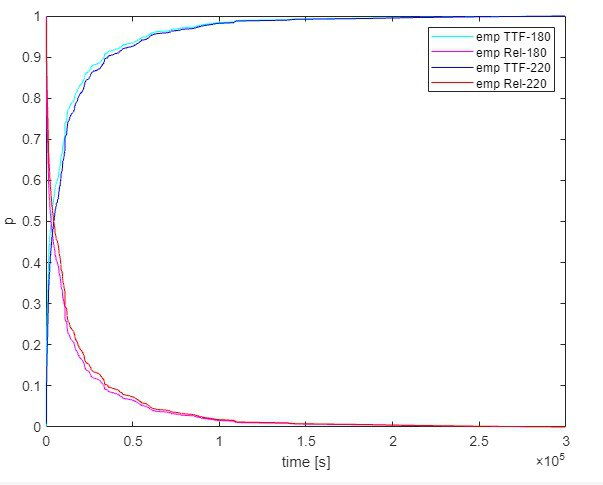
\includegraphics[width=\textwidth]{img/ch6/merc_ttf.png}
    \caption{Reliability Mercury con $W=180$ e $W=220$}
    \label{fig:merc_reliability}
\end{figure}

In seguito, è stata effettuata un'analisi per trovare la distribuzione che meglio rappresenta la Reliability empirica, con lo scopo di comprendere la natura dei fallimenti presenti nel sistema.

In particolare, è stato provato il \textit{fitting} per le seguenti distribuzioni:
\begin{itemize}
    \item \textbf{Esponenziale} (\cref{fig:merc_fit_exp}): i fallimenti sono \textit{memory less} e con \textit{failure rate} costante;
    \item \textbf{Iper-esponenziale}(\cref{fig:merc_fit_iperexp}): i fallimenti sono dovuti a più cause tra loro indipendenti;
    \item \textbf{Weibull}(\cref{fig:merc_fit_weibull}): con questa
    distribuzione si modellano i fallimenti con memoria di componenti
    elettronici;
\end{itemize}

\begin{figure}[H]
    \centering
    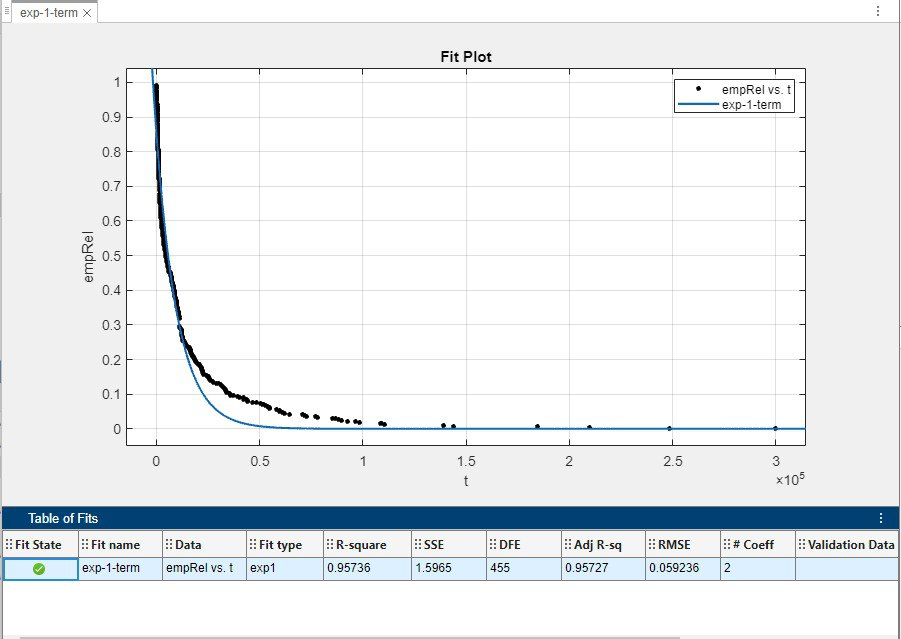
\includegraphics[width=\textwidth]{img/ch6/merc_fit_exp.png}
    \caption{Fit realiability Mercury con una distribuzione esponenziale}
    \label{fig:merc_fit_exp}
\end{figure}

\begin{figure}[H]
    \centering
    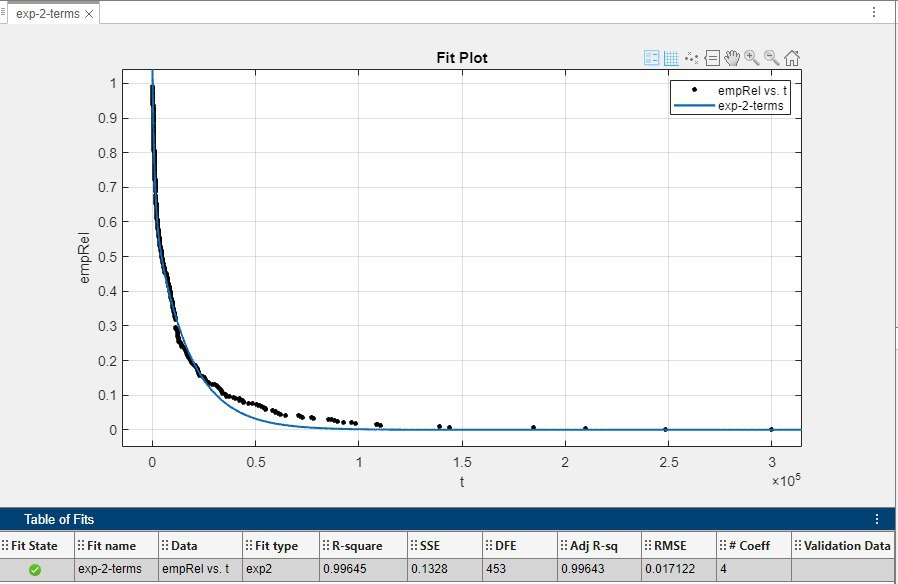
\includegraphics[width=\textwidth]{img/ch6/merc_fit_iperexp.png}
    \caption{Fit realiability Mercury con una distribuzione iper-esponenziale}
    \label{fig:merc_fit_iperexp}
\end{figure}

\begin{figure}[H]
    \centering
    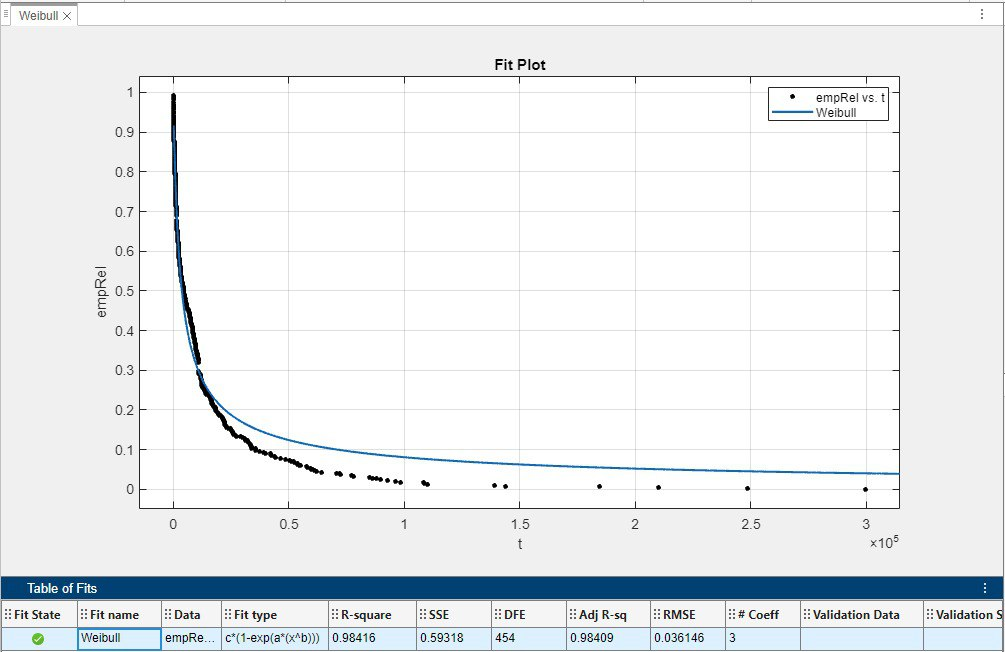
\includegraphics[width=\textwidth]{img/ch6/merc_fit_weibull.png}
    \caption{Fit realiability Mercury con una distribuzione weibull}
    \label{fig:merc_fit_weibull}
\end{figure}


\begin{table}[H]
\centering
    \begin{tabular}{|c|c|c|}
    \hline
    \multicolumn{1}{|c|}{\textbf{Curva}} &
    \multicolumn{1}{|c|}{\textbf{$R^2$}} &
    \multicolumn{1}{|c|}{\textbf{SSE}}
    \tabularnewline \hline

Esponenziale & $0.9573$ & $1.5965$   \tabularnewline \hline
Iper-esponenziale & $0.9964$ &  $0.1328$  \tabularnewline \hline
Weibull & $0.9841$ &  $0.5931$  \tabularnewline \hline
\end{tabular}
\caption{$R^2$ e SSE ottenuti dal fitting delle distribuzioni esponenziali, iper-esponenziali e Weibull}
\label{tab:merc_fit_parameters}
\end{table}

A valle della valutazione effettuata, osservando l'\textit{R-Square} e SSE in \cref{tab:merc_fit_parameters},  è possibile affermare che la distribuzione che meglio approssima la reliability empirica è una iper-esponenziale. 

Come ulteriore conferma è stato effettuato il test di Kolmogorov-Smirnov per le tre distribuzioni.

\begin{table}[H]
\centering
    \begin{tabular}{|c|c|c|}
    \hline
    \multicolumn{1}{|c|}{\textbf{Curva}} &
    \multicolumn{1}{|c|}{\textbf{H}} &
    \multicolumn{1}{|c|}{\textbf{P-Value}}
    \tabularnewline \hline

Esponenziale & $1$ & $0.68 \cdot10^{-4}$   \tabularnewline \hline
Iper-esponenziale & $0$ &  $0.7105$  \tabularnewline \hline
Weibull & $0$ &  $0.153$  \tabularnewline \hline
\end{tabular}
\caption{Esito test Kolmogorov-Smirnov}
\label{tab:ks_mercury}
\end{table}


\subsection{Analisi Collisions \& Truncations}

Proseguendo con $W=220$, sono state effettuate analisi per trovare collisioni e troncamenti all'interno delle tuple.

Per trovare una probabile collisione sono state esaminate le tuple a lunghezza maggiore, cercando eventi apparentemente slegati tra loro. 

Una probabile collisione è mostrata in \cref{fig:merc_collision} nella tupla 322, dove è possibile notare eventi relativi ai nodi di computazione \textit{tg-c401} e \textit{tg-c669} insieme a quelli del nodo di login \textit{tg-login3}, apparentemente slegati tra loro.
\begin{figure}[H]
    \centering
    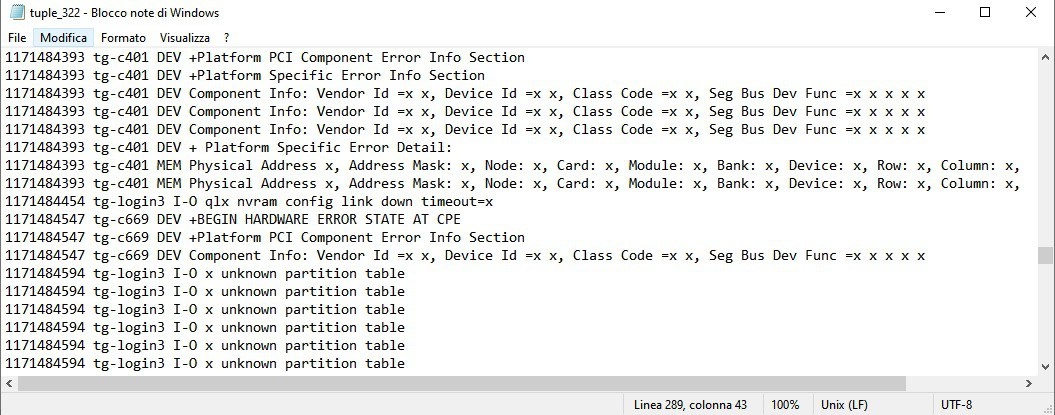
\includegraphics[width=\textwidth]{img/ch6/merc_collision.png}
    \caption{Esempio di probabile collisione per Mercury con $W=220$}
    \label{fig:merc_collision}
\end{figure}


Un esempio di probabile \textit{truncation} è mostrato in \cref{fig:merc_truncation}, dove è possibile notare che nelle tuple $66,67,68$ è presente lo stesso tipo di errore, di tipo NET, relativo allo stesso nodo \textit{tg-master}. 
\begin{figure}[H]
    \centering
    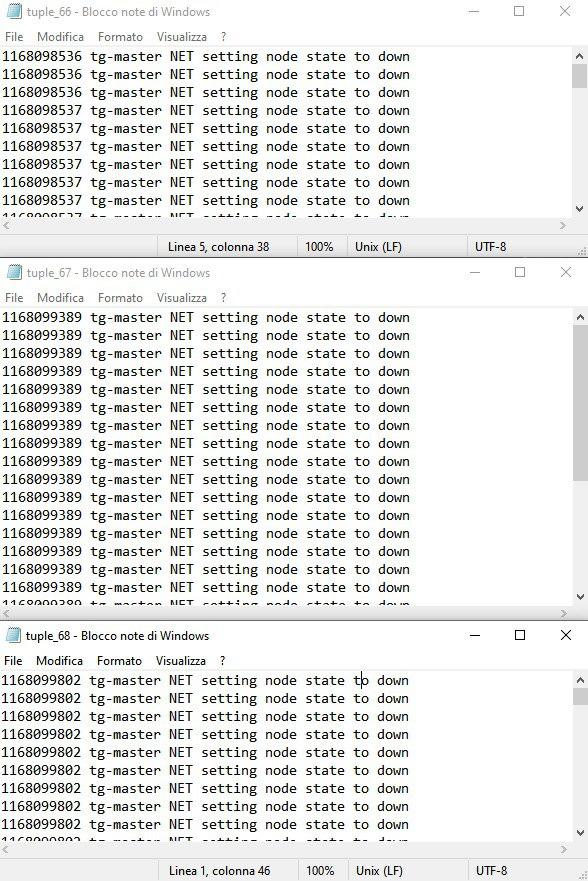
\includegraphics[width=0.8\textwidth]{img/ch6/merc_truncation.png}
    \caption{Esempio di probabile troncamento per Mercury con $W=220$}
    \label{fig:merc_truncation}
\end{figure}


\subsection{Ulteriori Analisi}

 \paragraph{Studio della Window size per nodi e categorie}
 Si vuole stabilire se sia possibile usare la stessa $W$ per i diversi nodi e le categorie di Mercury. 

Dopo una fase di filtraggio sono stati identificati i quattro nodi con più errori del sistema, ed è stata svolta una sensitivity analysis simile a quella presente nelle sezioni precedenti. 
I nodi scelti sono:
\begin{itemize}
    \item tg-c401
    \item tg-c572
    \item tg-master
    \item tg-s044
\end{itemize}


Dai risultati in \cref{fig:comp_windows-size_per-nodo} è possibile notare come per i diversi nodi non sia possibile scegliere una \textit{window size} unica e ottimale. 

\begin{figure}[H]
    \centering
    \begin{subfigure}{.5\textwidth}
        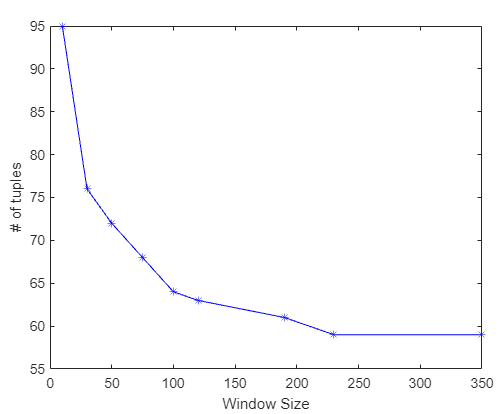
\includegraphics[width=\linewidth]{img/ch6/merc_cmaster-wsize.png}
        \caption{Nodo tg-master}
    \end{subfigure}\hfil
    \begin{subfigure}{.5\textwidth}
         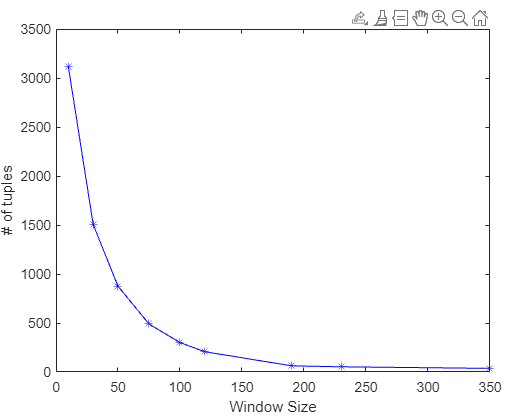
\includegraphics[width=\textwidth]{img/ch6/merc_c401-wsize.png}
         \caption{Nodo tg-c401}
    \end{subfigure}

    \begin{subfigure}{.5\textwidth}
        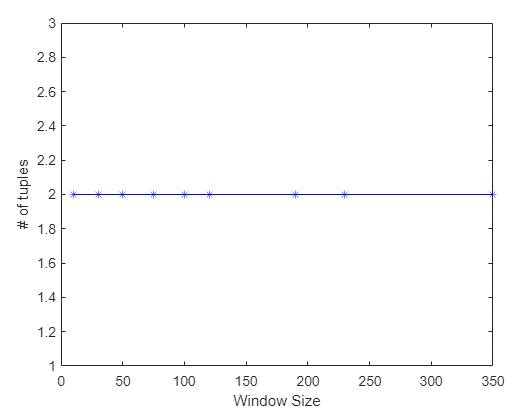
\includegraphics[width=\linewidth]{img/ch6/merc_c572-wsize.png}
        \caption{Nodo tg-master}
    \end{subfigure}\hfil
    \begin{subfigure}{.5\textwidth}
         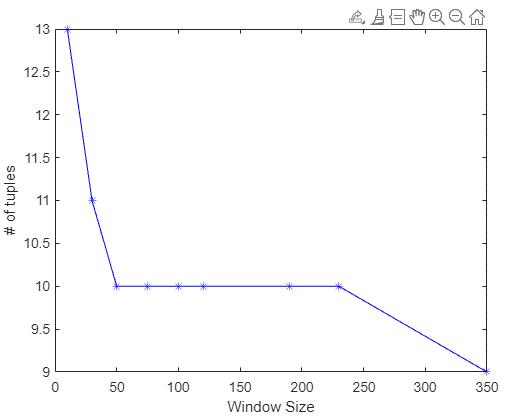
\includegraphics[width=\textwidth]{img/ch6/merc_s044-wsize.png}
         \caption{Nodo tg-c401}
    \end{subfigure}

    \caption{Comparazione window size per nodo}
    \label{fig:comp_windows-size_per-nodo}
\end{figure}


Per quanto riguarda invece le categorie di errore i risultati sono mostrati in \cref{eq:coal_window}, analizzando sempre le prime quattro in termini di numero di errori:
\begin{itemize}
    \item DEV
    \item IO
    \item NET
    \item MEM
    \item PRO
\end{itemize}

In questo caso una finestra vicina a 220 potrebbe andare bene per le categorie DEV, MEM e NET, ma risulta inadatta per I/O e PRO. 

\begin{figure}[H]
    \centering
    \begin{subfigure}{.5\textwidth}
        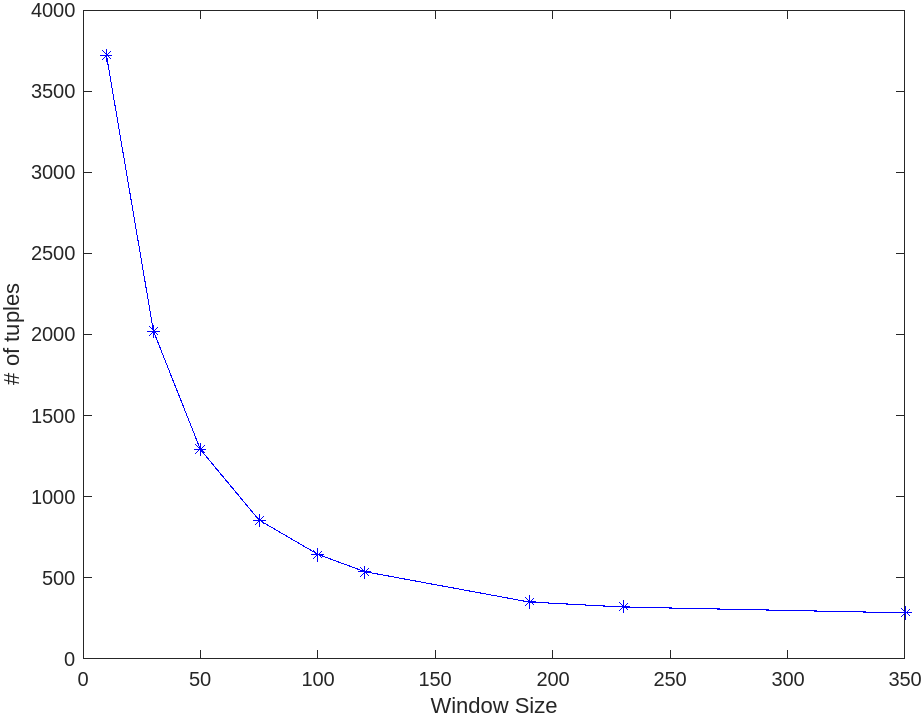
\includegraphics[width=\linewidth]{img/ch6/merc_dev-wsize.png}
        \caption{Categoria DEV}
    \end{subfigure}\hfil
    \begin{subfigure}{.5\textwidth}
         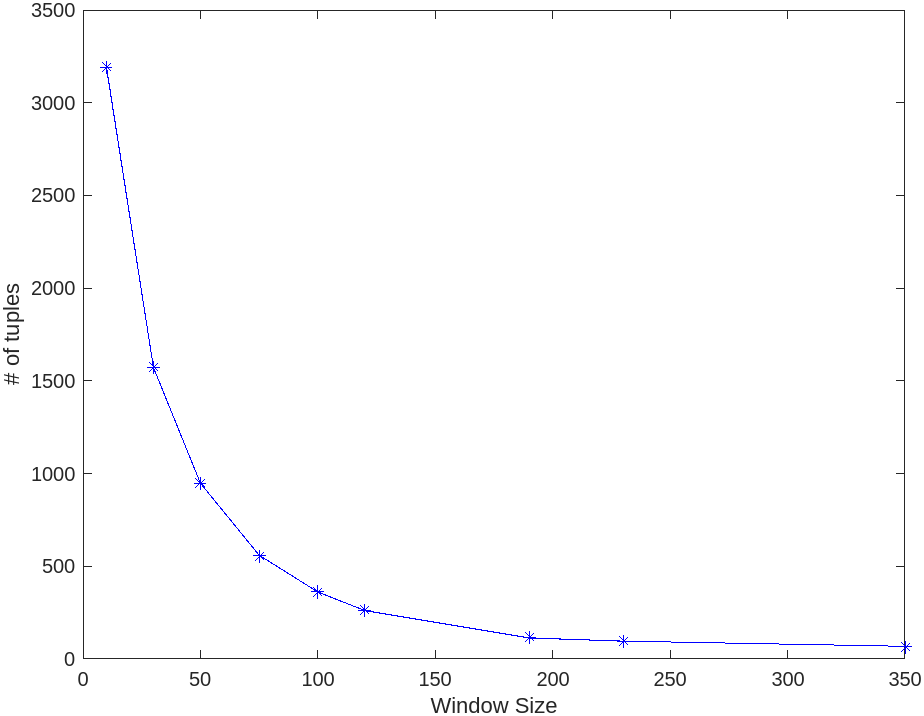
\includegraphics[width=\textwidth]{img/ch6/merc_mem-wsize.png}
         \caption{Catergoria MEM}
    \end{subfigure}

    \begin{subfigure}{.5\textwidth}
        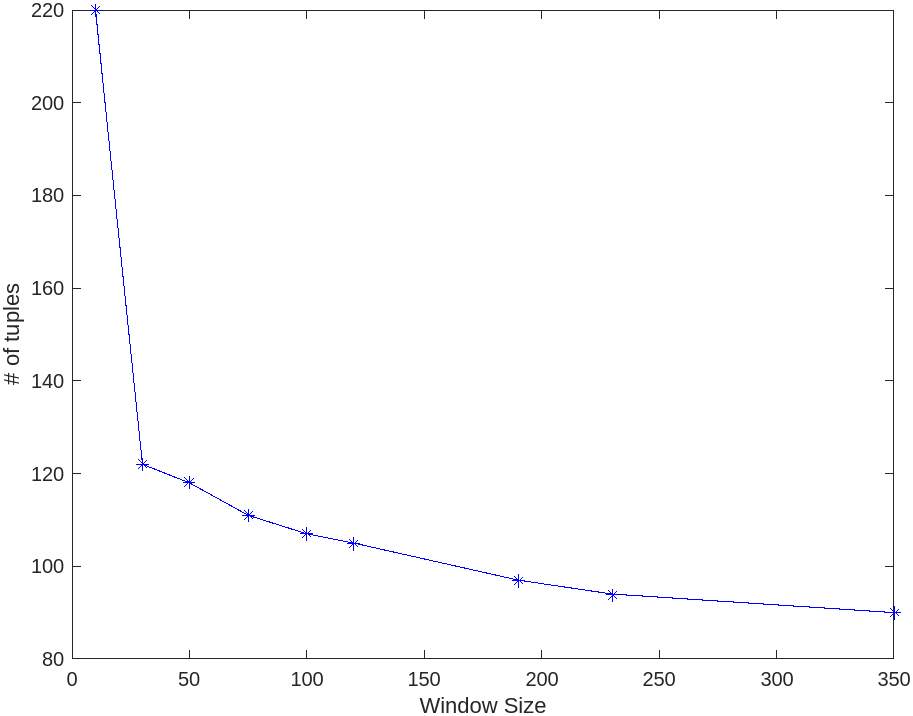
\includegraphics[width=\linewidth]{img/ch6/merc_io-wsize.png}
        \caption{Catergoria I/O}
    \end{subfigure}\hfil
    \begin{subfigure}{.5\textwidth}
         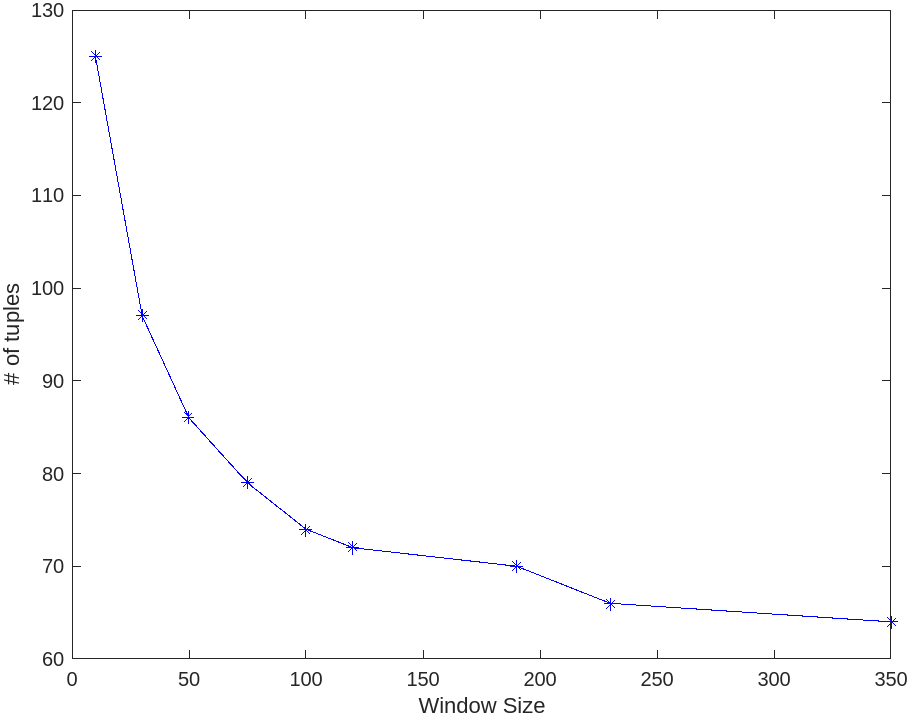
\includegraphics[width=\textwidth]{img/ch6/merc_net-wsize.png}
         \caption{Catergoria NET}
    \end{subfigure}

    \begin{subfigure}{.6\textwidth}
         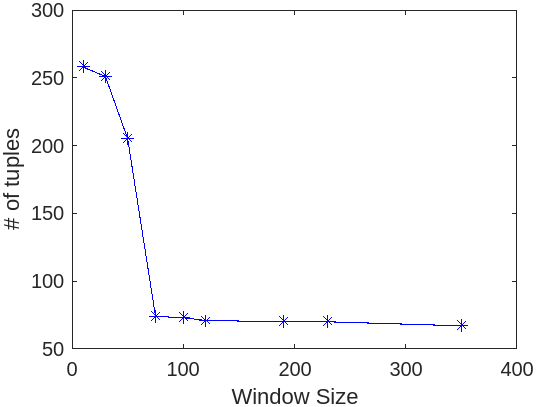
\includegraphics[width=\textwidth]{img/ch6/merc_pro-wsize.png}
         \caption{Catergoria PRO}
    \end{subfigure}

    \caption{Comparazione window size per categorie}
\end{figure}


\paragraph{Relazione tra system reliability e node reliability}

Al fine di comparare la reliability del sistema a quella dei nodi è stata effettuata un'analisi del TTF-empirico per questi ultimi, a partire dagli interarrivals filtrati. 

Come nelle sezioni precedenti, è stata effettuata in seguito una procedura di fitting, al termine della quale sono state individuate $4$ curve iper-esponenziali, rappresentanti le reliability dei nodi.

In \cref{fig:merc_rel_comp} è possibile notare come il nodo computazionale C401 abbia una reliability peggiore di quella del sistema totale, tant'è vero che la maggior parte degli errori nei log sono suoi.
Gli altri nodi si trovano al di sopra della reliability del sistema a partire da un certo istante di tempo.
Si noti che il nodo C572 non è presente nel grafico poichè, essendo composto da sole due tuple, non è stato possibile effettuare il fitting o rappresentarlo graficamente. 

\begin{figure}[H]
    \centering
    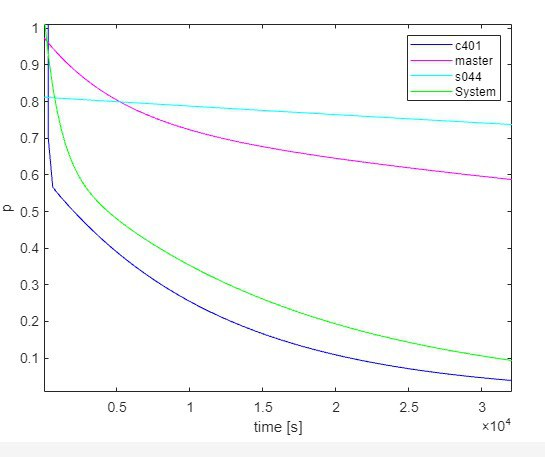
\includegraphics[width=\textwidth]{img/ch6/merc_rel_comp.png}
    \caption{Comparazione reliability del sistema Mercury con quella dei $4$ nodi analizzati}
    \label{fig:merc_rel_comp}
\end{figure}


\paragraph{Dependability Bottleneck}

Come mostrato nelle sezioni precedenti, il nodo che più contribuisce al numero di errori, e che peggiora la reliability del sistema generale è C401.

In \cref{fig:merc_error} si può notare che il nodo C401 contribuisce per più del 77\% degli errori.

\begin{figure}[H]
    \centering
    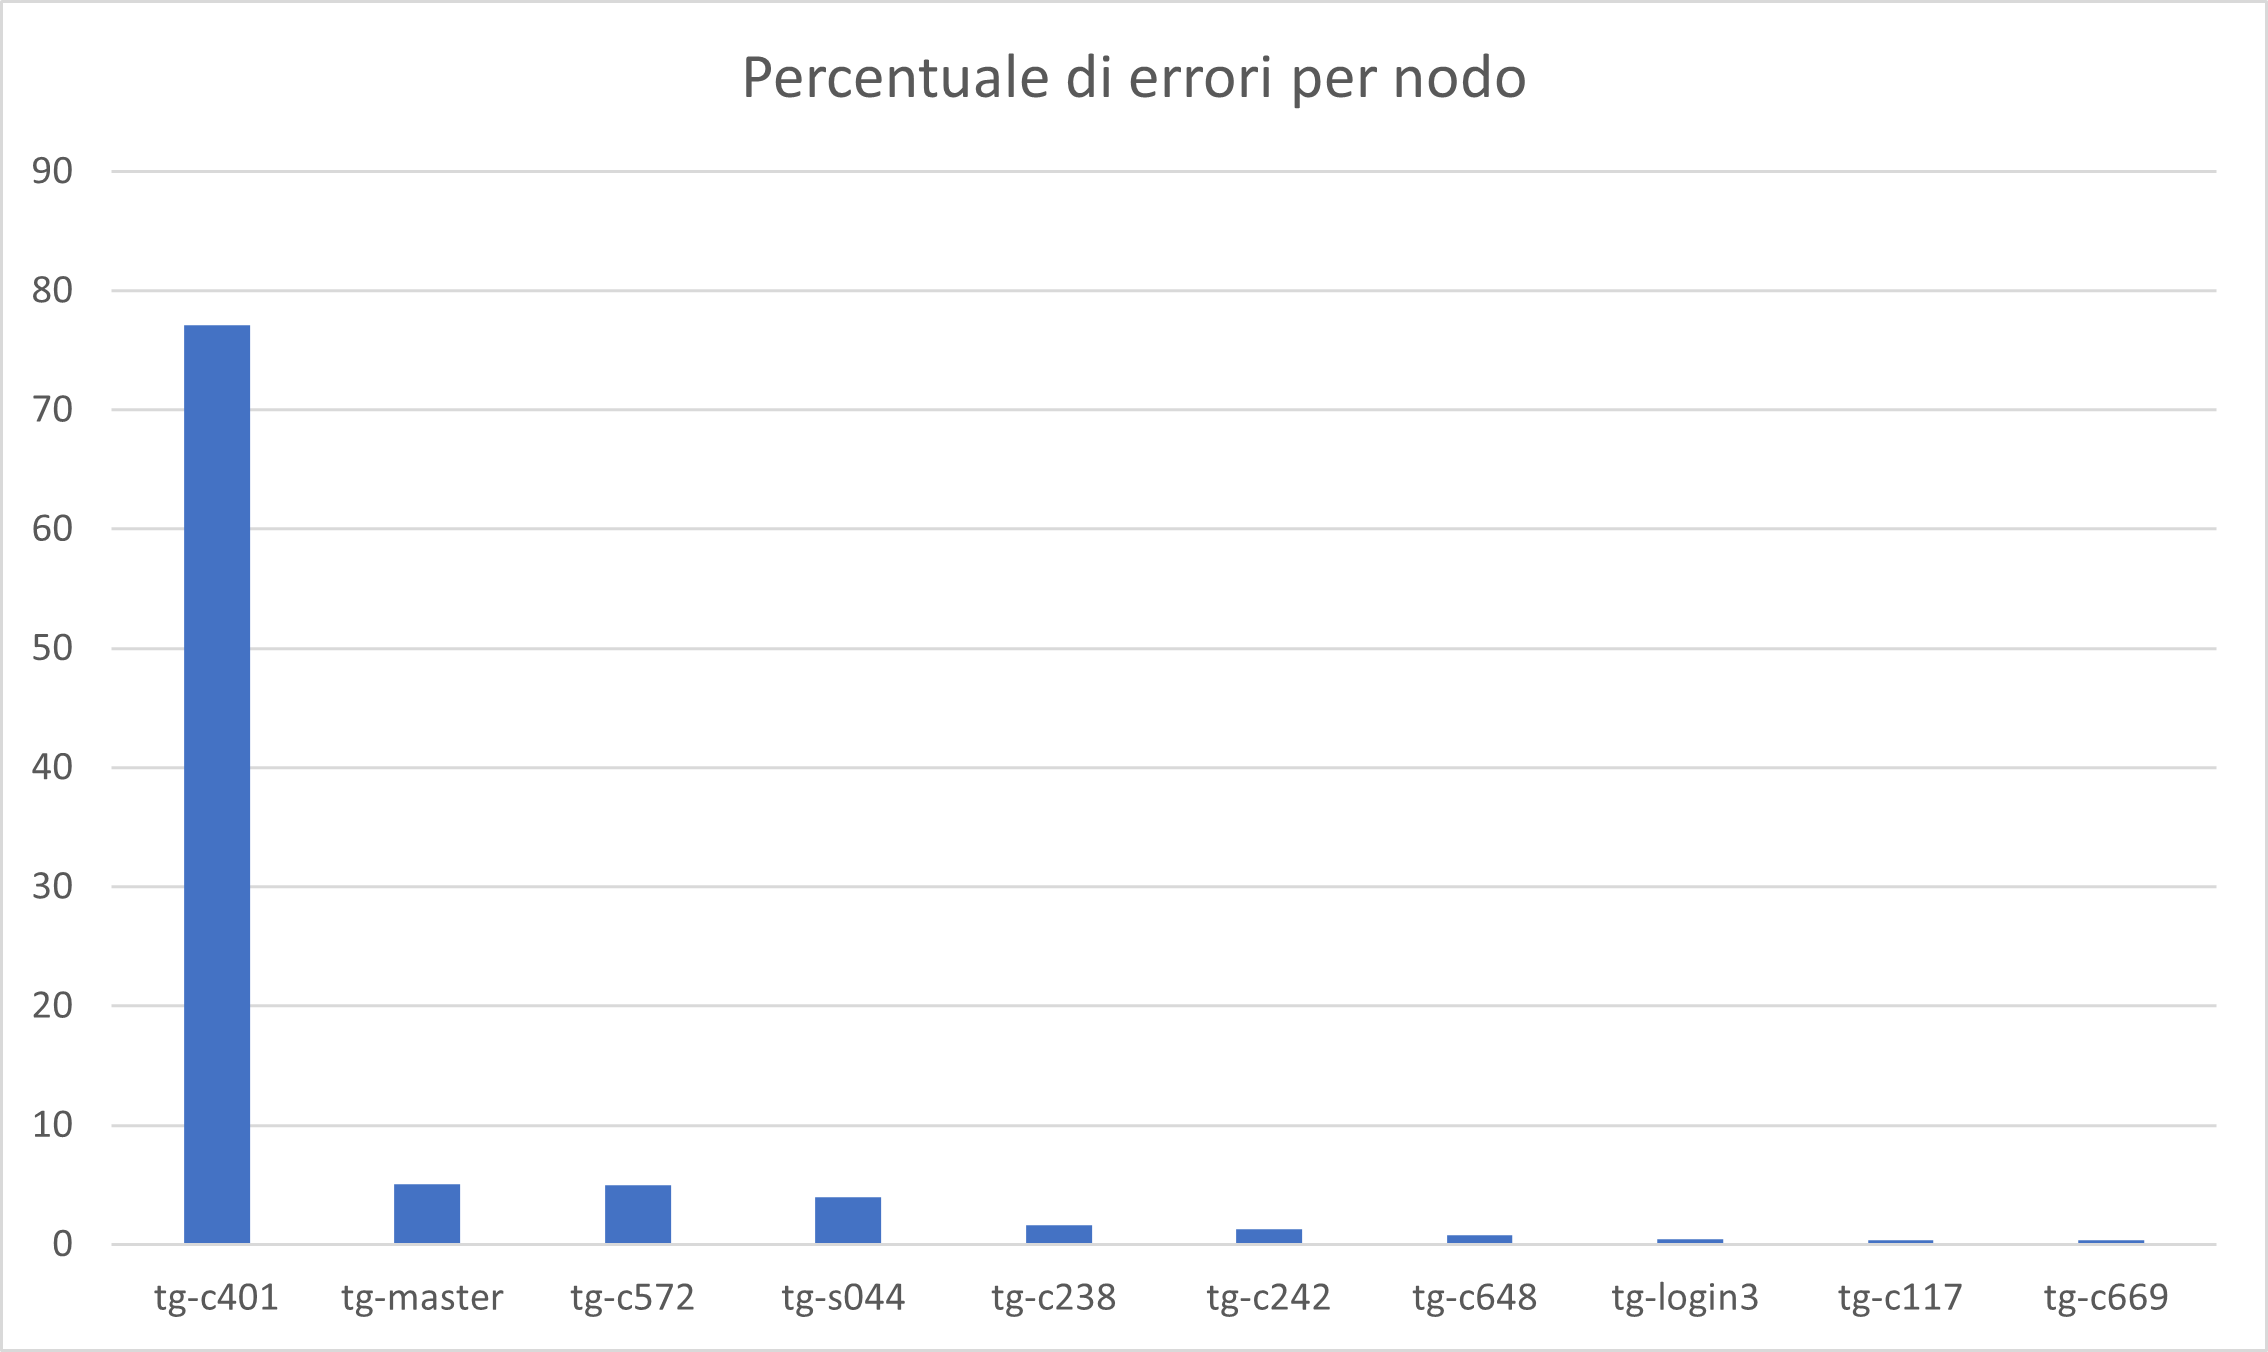
\includegraphics[width=\textwidth]{img/ch6/merc_errori.png}
    \caption{Percentuale di errori per nodo}
    \label{fig:merc_error}
\end{figure}

\paragraph{Reliability di nodi dello stesso tipo}

Sono stati esaminati due nodi di tipo computazionale:
\begin{itemize}
    \item C401
    \item C238
\end{itemize}

Dopo aver trovato la reliability empirica, ed aver fatto il fitting su una distribuzione iper-esponenziale, è possibile notare che, nonostante le differenze nell'andamento della curva vicino l'origine, la gran parte dei punti esaminati si trova sul tratto verticale che fa scendere quasi immediatamente la reliability. In questo senso si possono dire comparabili, anche se ovviamente C401 contribuisce per un numero molto maggiori di errori. 


\begin{figure}[H]
    \centering
    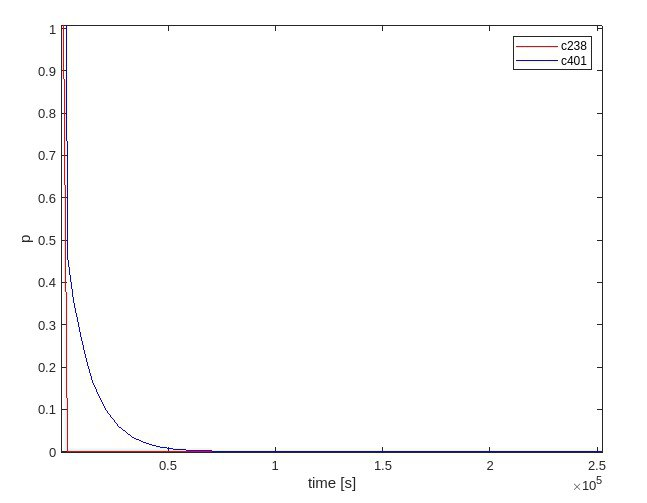
\includegraphics[width=0.8\textwidth]{img/ch6/merc_comp_c238vs401.png}
    \caption{Confronto reliability nodo \textit{tg-c401} e nodo \textit{tg-c238}}
    \label{fig:c238vsc401}
\end{figure}

\paragraph{Relazione tra tipo di errore e nodo}

Analizzando i \textit{fault} per categoria si trova che i nodi computazionali sono responsabili per la maggior parte degli errori di tipo \textit{DEV}, \textit{MEM} e \textit{PRO} (\cref{fig:err_calc_node}). Gli errori relativi alla rete (NET) sono per la maggior parte generati dal nodo \textit{tg-master} (\cref{fig:err_calc_node}).

Per quanto riguarda gli errori di tipo I/O, si può notare che sono dovuti principalmente al nodo di storage \textit{tg-s044} (\cref{fig:err_storage_node}), con la parte rimanente bilanciata tra altri tipi di nodi.

\begin{figure}[H]
    \centering
    \begin{subfigure}{.5\textwidth}
        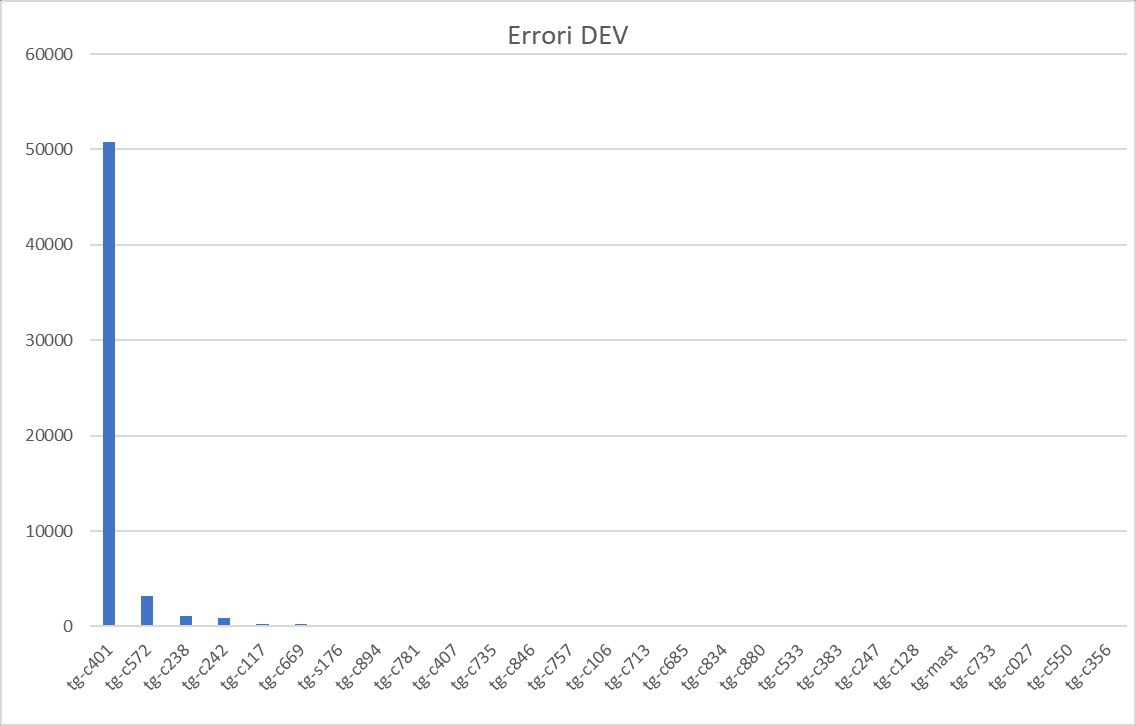
\includegraphics[width=\linewidth]{img/ch6/merc_dev_by_node.png}
        \caption{Errori tipo DEV}
    \end{subfigure}\hfil
    \begin{subfigure}{.5\textwidth}
        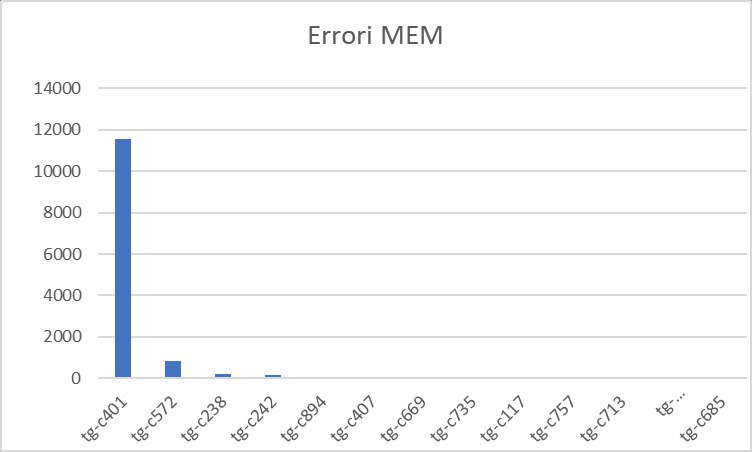
\includegraphics[width=\linewidth]{img/ch6/merc_mem_by_node.png}
        \caption{Errori tipo MEM}
    \end{subfigure}
    \begin{subfigure}{.6\textwidth}
        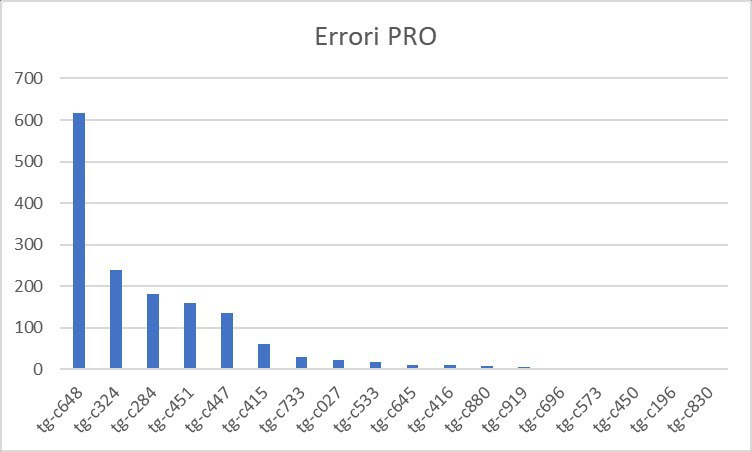
\includegraphics[width=\linewidth]{img/ch6/merc_pro_by_node.png}
        \caption{Errori tipo PRO}
    \end{subfigure}
    \caption{Errori di cui sono maggiormente responsabili i nodi di calcolo}
    \label{fig:err_calc_node}
\end{figure}


\begin{figure}[H]
    \centering
    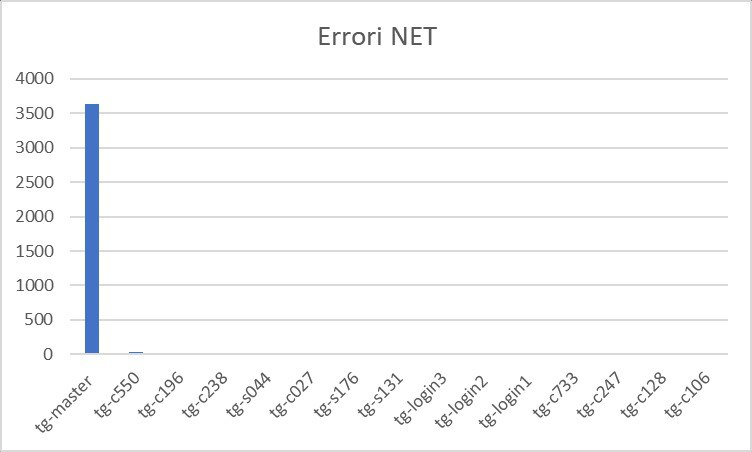
\includegraphics[width=0.9\textwidth]{img/ch6/merc_net_by_node.png}
    \caption{Errori di tipo NET}
    \label{fig:err_master_node}
\end{figure}


\begin{figure}[H]
    \centering
    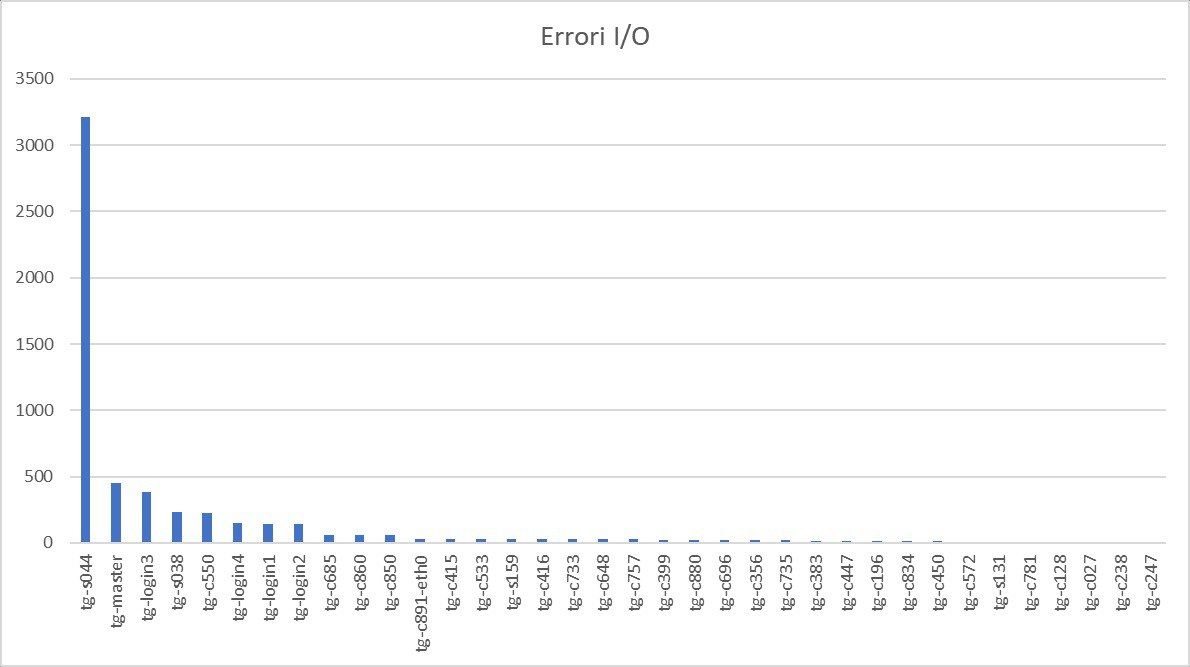
\includegraphics[width=0.9\textwidth]{img/ch6/merc_io_by_node.png}
    \caption{Errori di tipo I/O}
    \label{fig:err_storage_node}
\end{figure}

\clearpage
\section{BlueGene/L}

Il super-calcolatore \textit{Blue Gene/L} presenta un'architettura che consiste in 64 unità contenitrici dette Rack ciascuna delle quali costituita da 2 Midplane. Ogni Midplane possiede 16 Node Card ognuna di esse caratterizzata da 16 unità di calcolo computazionale, inoltre alcuni midplane presentano una card I/O.

\begin{figure}[H]
    \centering
    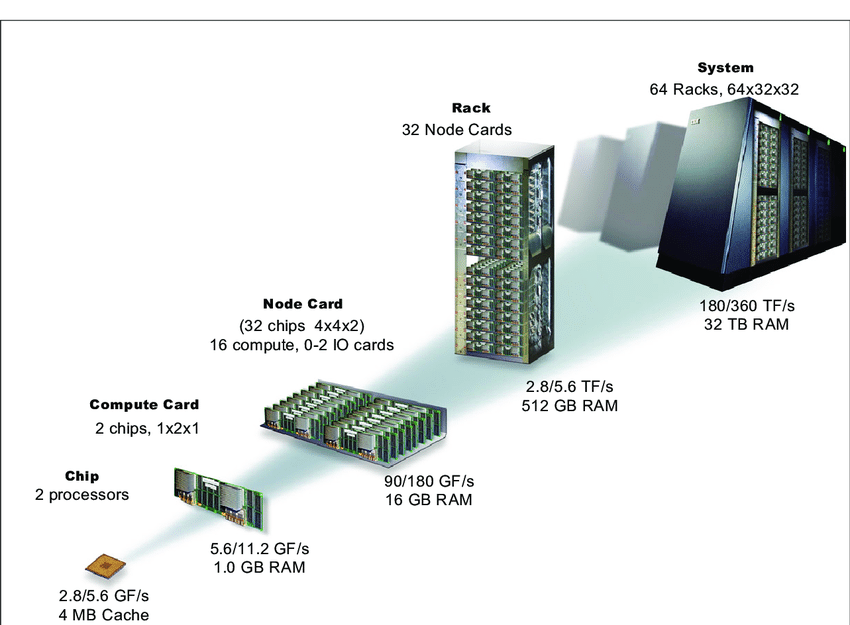
\includegraphics[width=0.8\textwidth]{img/ch6/BG_L_architecture.png}
    \caption{Architettura del super-calcolatore BlueGene/L}
    \label{fig:bgl_arch}
\end{figure}

Il file di log in ingresso BGLErrorLog.txt contiene $125624$ entry già filtrate, sono infatti riportate le entry relative ai soli errori fatali. Ogni entry ha il formato \textit{timestamp - nodo di origine - card di origine - messaggio di errore}.



\subsection{Temporal Coalescence}
Similmente a quanto fatto per Mercury, al fine di semplificare l'analisi dei log del sistema è stata applicata la tecnica della coalescenza temporale raggruppando le entry riconducibili allo stesso fault secondo una determinata finestra temporale $W$, determinata, anche in questo caso, tramite una \textit{Sensitivity Analysis}, calcolando il numero di tuple generate a seconda di multipli valori della \textit{window size}.

\begin{figure}[H]
    \centering
    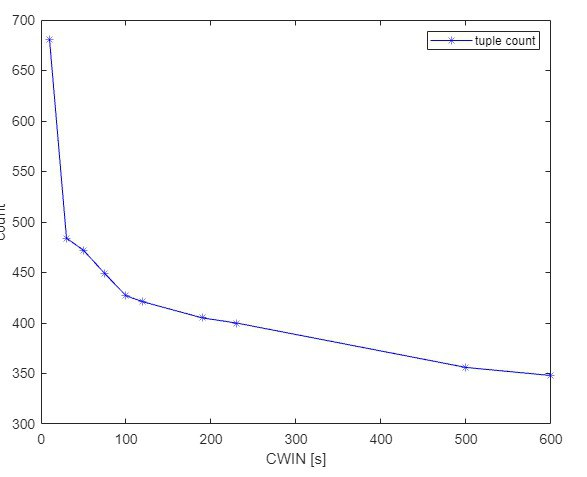
\includegraphics[width=0.8\textwidth]{img/ch6/blg_cwin.png}
    \caption{}
    \label{fig:blg_cwin}
\end{figure}

Ponendoci leggermente a destra del punto di knee sono stati scelti i seguenti valori per $W$:
\begin{itemize}
    \item $W=180$
    \item $W=220$
\end{itemize}

Per entrambe le \textit{window size} sono state generate le tuple e le seguenti statistiche:
\begin{itemize}
    \item Interarrivals: tempi di interarrivo tra le tuple (TTF).
    \item Starting points: timestamp del punto di inizio della tupla.
    \item Lengths: durata dei fallimenti e quindi la lunghezza delle singole tuple.
\end{itemize}


\subsection{Reliability}
Procediamo dunque con una stima empirica della reliability del sistema utilizzando il TTF calcolato a partire dagli \textit{interarrivals} ottenuti tramite l'analisi riportata nella sezione precedente.
In \cref{fig:bgl_reliability} è possibile notare come la reliability con $W=180$ sia migliore di quella con $W=220$. 
\begin{figure}[H]
    \centering
    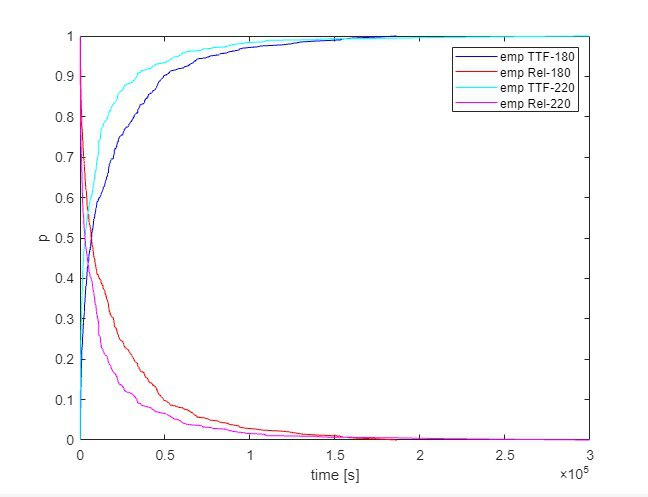
\includegraphics[width=\textwidth]{img/ch6/blg_ttf.png}
    \caption{Reliability BlueGeen/L con $W=180$ e $W=220$}
    \label{fig:bgl_reliability}
\end{figure}

Considerando la TTF e la Reliability empirica per $W=180$, è stata effettuata un'analisi per trovare la distribuzione che meglio rappresenta la Reliability empirica del super-calcolatore BlueGeen/L, con lo scopo di comprendere la natura dei fallimenti presenti nel sistema.

Anche in questo caso è stato provato il \textit{fitting} per le seguenti distribuzioni:
\begin{itemize}
    \item \textbf{Esponenziale} (\cref{fig:blg_fit_exp}): i fallimenti sono \textit{memory less} e con \textit{failure rate} costante;
    \item \textbf{Iper-esponenziale }(\cref{fig:blg_fit_iperexp}): i fallimenti sono dovuti a più cause tra loro indipendenti;
    \item \textbf{Weibull}(\cref{fig:blg_fit_weibull}): con questa
    distribuzione si modellano i fallimenti con memoria di componenti
    elettronici;
\end{itemize}

\begin{figure}[H]
    \centering
    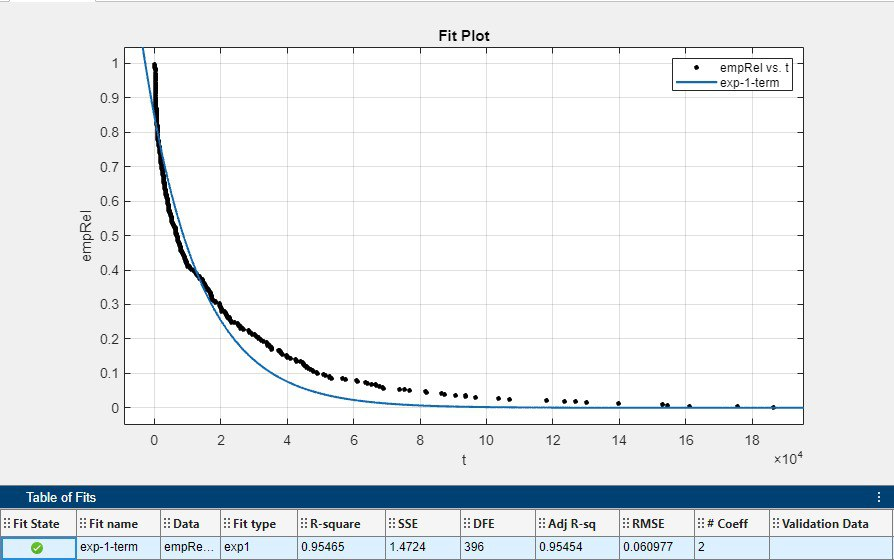
\includegraphics[width=\textwidth]{img/ch6/blg_fit_exp.png}
    \caption{Fit realiability BlueGeen/L con una distribuzione esponenziale}
    \label{fig:blg_fit_exp}
\end{figure}

\begin{figure}[H]
    \centering
    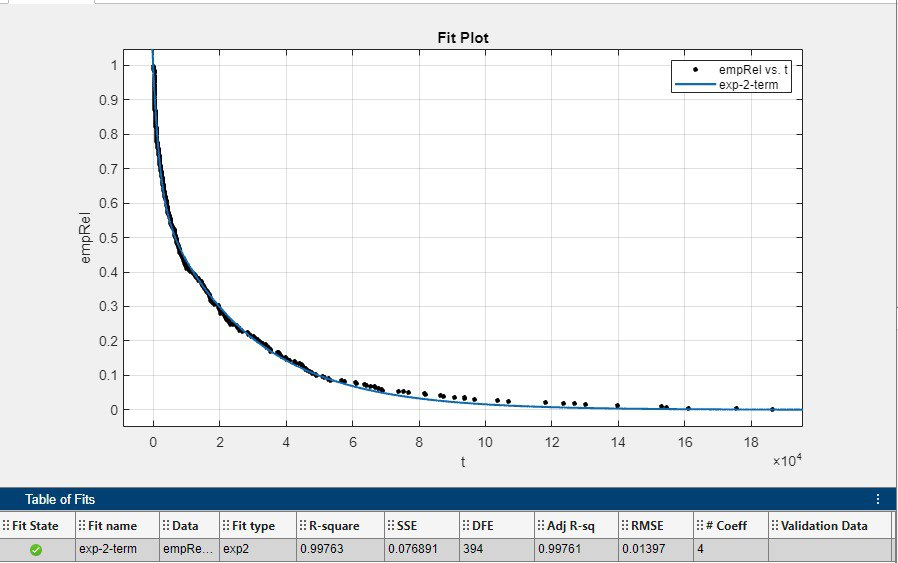
\includegraphics[width=\textwidth]{img/ch6/blg_fit_iperexp.png}
    \caption{Fit realiability BlueGeen/L con una distribuzione iper-esponenziale}
    \label{fig:blg_fit_iperexp}
\end{figure}

\begin{figure}[H]
    \centering
    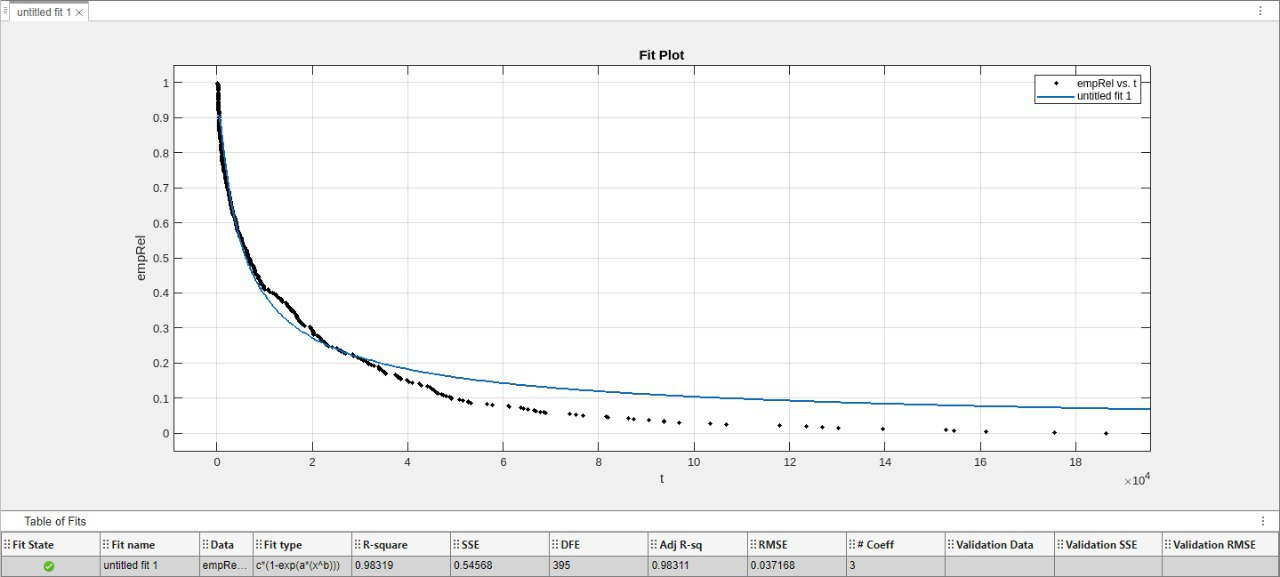
\includegraphics[width=\textwidth]{img/ch6/blg_fit_weibull.png}
    \caption{Fit realiability BlueGeen/L  con una distribuzione Weibull}
    \label{fig:blg_fit_weibull}
\end{figure}

\begin{table}[H]
\centering
    \begin{tabular}{|c|c|c|}
    \hline
    \multicolumn{1}{|c|}{\textbf{Curva}} &
    \multicolumn{1}{|c|}{\textbf{$R^2$}} &
    \multicolumn{1}{|c|}{\textbf{SSE}}
    \tabularnewline \hline

Esponenziale & $0.9546$ & $1.4724$   \tabularnewline \hline
Iper-esponenziale & $0.9976$ &  $0.0768$  \tabularnewline\hline
Weibull & $0.9832$ &  $0.5457$  \tabularnewline\hline

\end{tabular}
\caption{$R^2$ e SSE ottenuti dal fitting delle distribuzioni esponenziali ed iper-esponenziali}
\label{tab:blg_fit_parameters}
\end{table}


Osservando i valori relativi l'\textit{R-Square} e la SSE in \cref{tab:blg_fit_parameters},  è possibile affermare che la distribuzione che meglio approssima la reliability empirica è una iper-esponenziale. 

Come ulteriore conferma è stato effettuato il test di Kolmogorov-Smirnov per le due distribuzioni.

\begin{table}[H]
\centering
    \begin{tabular}{|c|c|c|}
    \hline
    \multicolumn{1}{|c|}{\textbf{Curva}} &
    \multicolumn{1}{|c|}{\textbf{H}} &
    \multicolumn{1}{|c|}{\textbf{P-Value}}
    \tabularnewline \hline

Esponenziale & $1$ & $2.7130 \cdot10^{-4}$   \tabularnewline \hline
Iper-esponenziale & $0$ &  $0.8016$  \tabularnewline \hline
Weibull & $0$ &  $0.10$  \tabularnewline \hline
\end{tabular}
\caption{Esito test Kolmogorov-Smirnov}
\label{tab:ks_blg}
\end{table}

\subsection{Analisi Collisions \& Truncations}

Proseguendo con $W=180$, sono state effettuate analisi per trovare collisioni e troncamenti all'interno delle tuple.

Per trovare una probabile collisione sono state esaminate le tuple a lunghezza maggiore, cercando eventi apparentemente slegati tra loro. 

Una probabile collisione è mostrata in \cref{fig:blg_collision} nella tupla 145, dove è possibile notare che le entry riportate in essa, stampate da card di I-O, non solo facciano riferimento a nodi appartenenti a Rack diversi (\textit{R62 ed R63}) ma sembrerebbero tra loro non correlate, in particolare i primi riportano un errore riconducibile ad un percorso errato o ad un file mancante, i restanti invece riportano un errore relativo alla dimensione eccessiva di un file.
\begin{figure}[H]
    \centering
    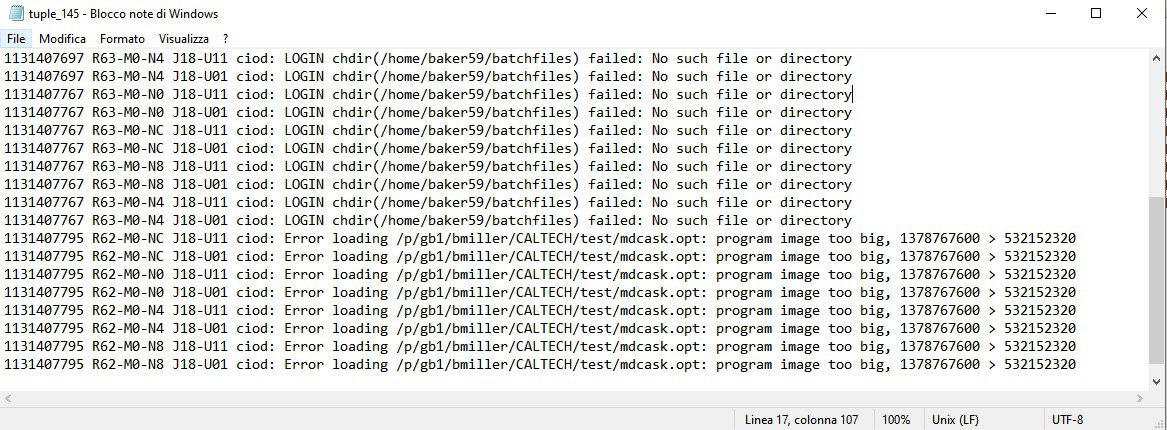
\includegraphics[width=\textwidth]{img/ch6/blg_collision.png}
    \caption{Esempio di probabile collisione per BlueGeen/L con $W=180$}
    \label{fig:blg_collision}
\end{figure}

Un esempio di probabile \textit{truncation} è mostrato in \cref{fig:blg_truncation} in cui è riportato il contenuto delle tuple $369,370,371,372$. Le entry riportate in esse riportano lo stesso messaggio d'errore e sono stampate dagli stessi nodi in un intervallo di tempo relativamente piccolo. 
\begin{figure}[H]
    \centering
    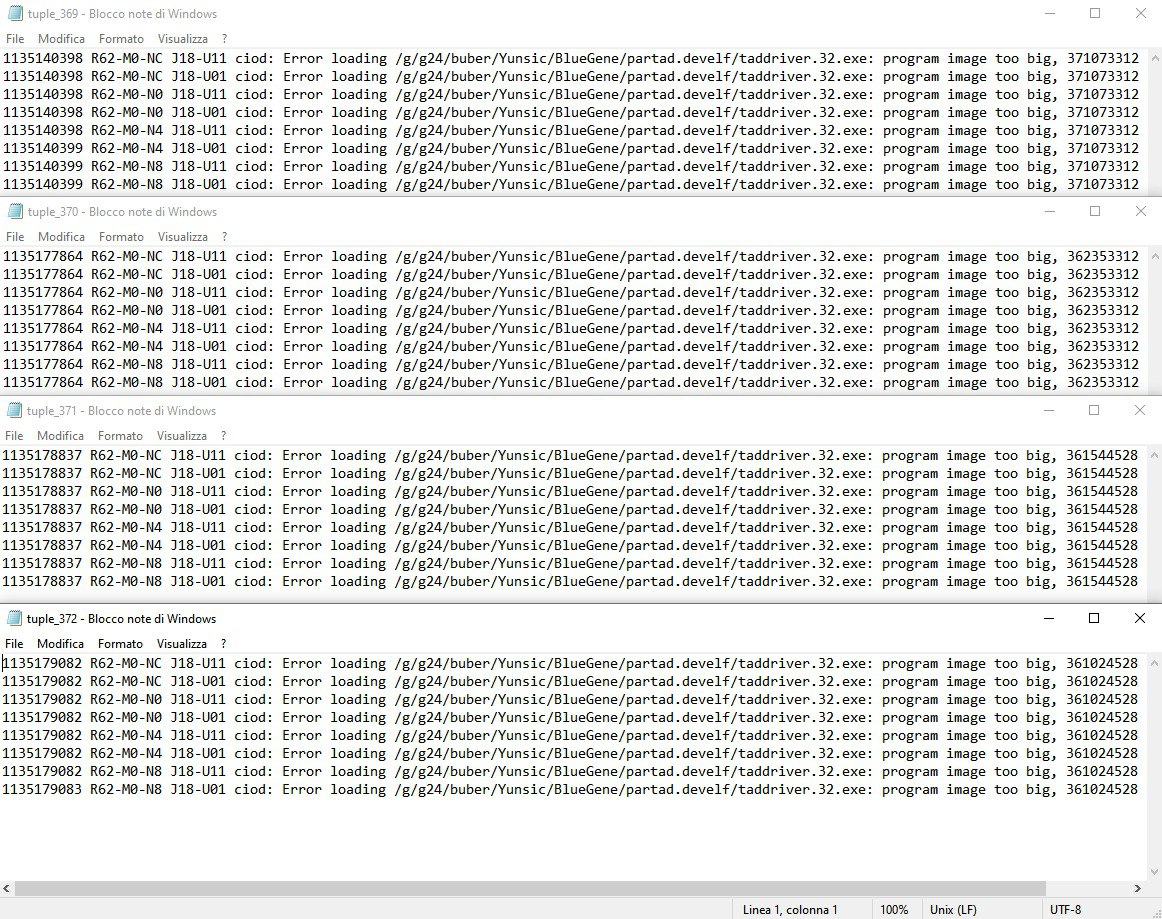
\includegraphics[width=0.8\textwidth]{img/ch6/blg_truncation.png}
    \caption{Esempio di probabile troncamento per BlueGeen/L con $W=180$}
    \label{fig:blg_truncation}
\end{figure}

\subsection{Ulteriori Analisi}
\paragraph{Studio della Window size per nodi}
Si vuole stabilire se sia possibile usare la stessa $W$ per i diversi nodi di BlueGeen/L. 

Dopo una fase di filtraggio sono stati identificati i quattro nodi con più errori del sistema, ed è stata svolta una sensitivity analysis simile a quella presente nelle sezioni precedenti. 
I nodi scelti sono:
\begin{itemize}
    \item R71-M0-N4
    \item R12-M0-N0 
    \item R63-M0-N2
    \item R03-M1-NF
\end{itemize}

Dai risultati in \cref{fig:comp_windows-size_per-nodo_bgl} è possibile notare come il valore $W=230$ potrebbe essere una scelta ottimale per la \textit{window size} per i nodi $R71-M0-N4,R12-M0-N0,R03-M1-NF$. Tuttavia osservando il grafico relativo al nodo $R63-M0-N2$ intuiamo come tale scelta potrebbe aumentare i fenomeni di collision delle entry non correlate nelle tuple rispetto ad una \textit{window size} più piccola per gli errori stampati. Ciò varrebbe per le sole entry stampate da questo specifico nodo.

\begin{figure}[H]
    \centering
    \begin{subfigure}{.5\textwidth}
        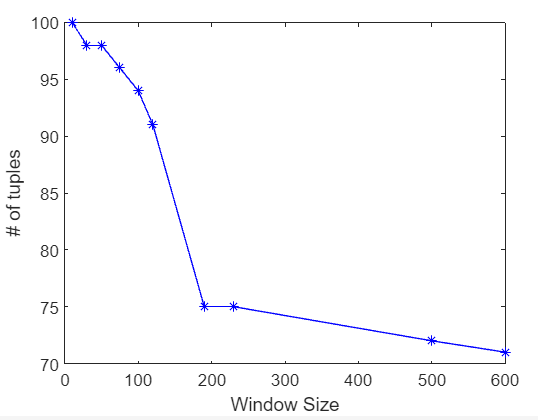
\includegraphics[width=\linewidth]{img/ch6/R71-M0-N4_cwin_numTuple.png}
        \caption{Nodo R71-M0-N4}
    \end{subfigure}\hfil
    \begin{subfigure}{.5\textwidth}
         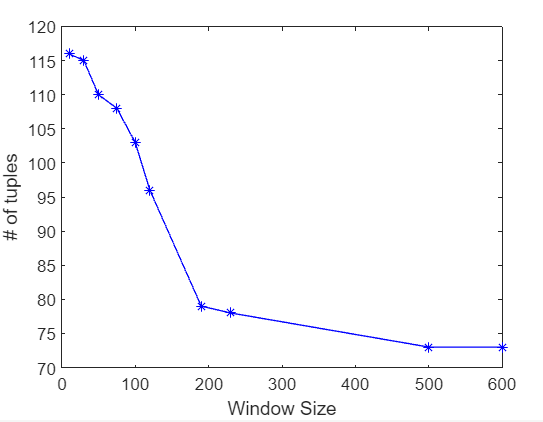
\includegraphics[width=\textwidth]{img/ch6/R12-M0-N0_cwin_numTuple.png}
         \caption{Nodo R12-M0-N0}
    \end{subfigure}

    \begin{subfigure}{.5\textwidth}
        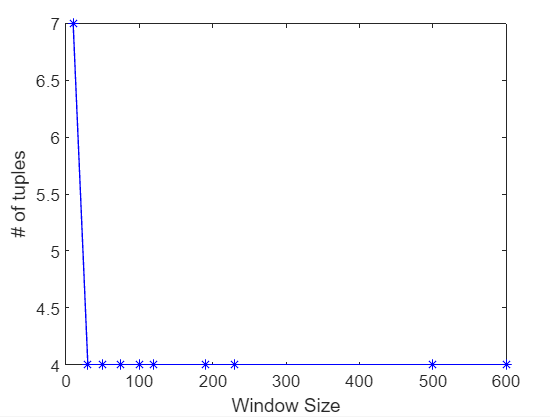
\includegraphics[width=\linewidth]{img/ch6/R63-M0-N2_cwin_numTuple.png}
        \caption{Nodo R63-M0-N2}
    \end{subfigure}\hfil
    \begin{subfigure}{.5\textwidth}
         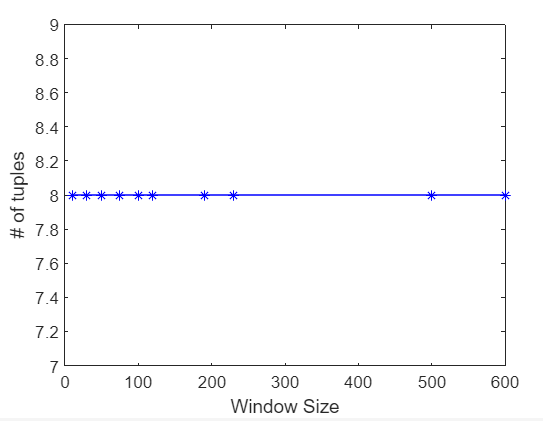
\includegraphics[width=\textwidth]{img/ch6/R03-M1-NF_cwin_numTuple.png}
         \caption{Nodo R03-M1-NF}
    \end{subfigure}
    \caption{Comparazione window size per nodo}
    \label{fig:comp_windows-size_per-nodo_bgl}
\end{figure}

\paragraph{Relazione tra system reliability e node reliability}
l fine di comparare la reliability del sistema a quella dei nodi è stata effettuata un'analisi del TTF-empirico per questi ultimi, a partire dagli interarrivals filtrati. 

Come nelle sezioni precedenti, è stata effettuata in seguito una procedura di fitting, al termine della quale sono state individuate $4$ curve iper-esponenziali, rappresentanti le reliability dei nodi.

In \cref{fig:bgl_comp}, è possibile notare come ci sia una sovrapposizione tra le reliability di BG/L con R12-M0-N0 ed R03-M1-NF con R71-M0-N40.
Gli altri nodi si trovano al di sopra della reliability del sistema.

\begin{figure}[H]
    \centering
    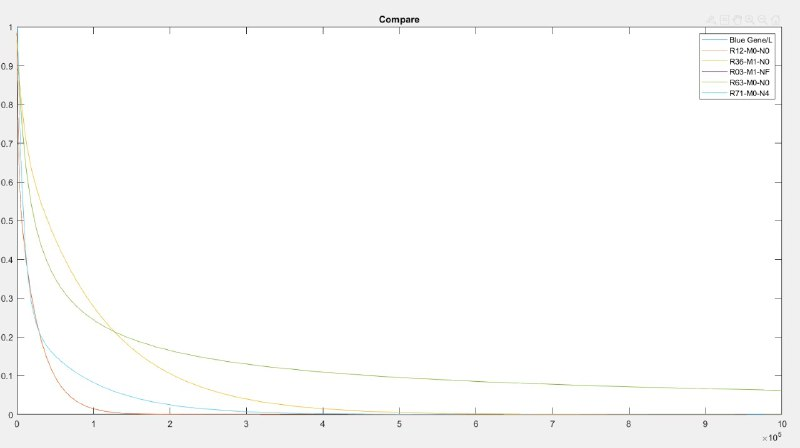
\includegraphics[width=.9\textwidth]{img/ch6/bgl_rel_comp.png}
    \caption{Confronto reliability nodi con quella del sistema per BlueGeen/L}
    \label{fig:bgl_comp}
\end{figure}


\paragraph{Dependability Bottleneck}

Dalle statistiche raccolte sui log di BGL i nodi più fallimentari risultano essere R71-M0-N4 e R12-M0-N0. 
È da notare che la gran parte dei fallimenti è da imputare alla scheda J18, responsabile delle operazioni di I/O, che può essere considerata il bottleneck del sistema. 

Per il resto i fallimenti sono distribuiti in maniera più bilanciata tra gli altri nodi rispetto a Mercury.







\end{document}e
